%%%%%%%%%%%%%%%%%%%%%%%%%%%
\chapter{Single-Variable Calculus, Vectors, and the Geometry of Space}

\section*{Introduction}

In this chapter, we begin our journey into multivariable calculus by revisiting core concepts from Calculus I and Calculus II. These reviews will serve as stepping stones as we enter into the world of ``high-dimensional thinking." Our goal is to build a solid foundation for understanding functions that involve several variables, expanding beyond the single-variable functions studied previously. Functions of multiple variables naturally arise in physics and engineering. This chapter will introduce functions like these that depend on multiple variables, setting the stage for exploring complex systems where outcomes are influenced by more than one parameter. \\ \\To engage with these new concepts, we will introduce vectors, essential tools for representing quantities with both magnitude and direction. Vectors are critical for understanding spatial relationships and navigating the geometry of three-dimensional space. We will cover the fundamental operations on vectors, including addition, scalar multiplication, dot product, and cross product, each with significant applications in describing physical forces, directions, and motions. Furthermore, this chapter will introduce the geometry of space, specifically three-dimensional coordinate systems. By exploring Cartesian, cylindrical, and spherical coordinates, we will establish methods to describe points, lines, planes, and surfaces in space. These systems provide multiple ways of visualizing and solving problems, especially in fields like engineering and physics, where spatial reasoning and high-dimensional analysis are vital. \\ \\ In summary, this chapter lays the groundwork for high-dimensional thinking, equipping students with the skills to analyze functions of several variables and understand the fundamental geometry of space. With a thorough review of Calculus I and II concepts, we’ll be ready to explore multivariable calculus, ultimately deepening our ability to model and interpret complex systems.
\newpage


\lecture{Review of Differential and Integral Calculus}



\subsection*{Review of Single-Variable Calculus}\index{Calculus}

\noindent Before we embark on multivariable calculus, it’s essential to have a strong command of foundational topics in single-variable calculus, along with proficiency in algebra. Mastery of differentiation, integration, and limits forms the backbone of the more advanced concepts we’ll explore in this course. Additionally, skill in handling complex algebraic expressions will be invaluable, as calculus problems frequently require careful algebraic manipulation. These topics should already be second nature:

\begin{enumerate}
    \item \textbf{Limits and Continuity:}
    
    \noindent A precise understanding of limits is fundamental. You should be comfortable calculating limits both algebraically and conceptually, as they underpin differentiation, integration, and continuity. Key ideas include the \(\varepsilon\)-\(\delta\) definition of a limit, one-sided limits, and limits approaching infinity.
    
    \item \textbf{Differentiation:}
    
    \noindent Differentiation techniques such as the power rule, product rule, quotient rule, and chain rule must be second nature. In multivariate calculus, you will extend these rules to partial derivatives and gradients. Familiarity with applications of derivatives—such as optimization, related rates, and curve sketching—is also critical, as these concepts generalize to higher dimensions.

    \item \textbf{Integration:}
    
    \noindent Integration techniques such as substitution, integration by parts, and partial fraction decomposition will reappear in multivariable settings. Definite and indefinite integrals, as well as their geometric interpretations (e.g., areas under curves), are fundamental. In multivariate calculus, we’ll extend these concepts to double and triple integrals over various regions.

    \item \textbf{Fundamental Theorem of Calculus:}
    
    \noindent A firm grasp of the Fundamental Theorem of Calculus is crucial. This theorem connects differentiation and integration, and its higher-dimensional analogs—like Green’s Theorem, Stokes’ Theorem, and the Divergence Theorem—are central topics in multivariate calculus.

    \item \textbf{Algebraic Skills:}
    
    \noindent Proficiency in manipulating algebraic expressions is indispensable. Be comfortable simplifying complex fractions, solving linear and quadratic equations, and working with exponential and logarithmic functions. Multivariable calculus often involves tedious algebraic steps, and fluency here will prevent errors.
\end{enumerate}

\noindent As we review these topics, consider how they might extend into three dimensions and beyond. For example, differentiation in higher dimensions involves calculating partial derivatives, gradients, and directional derivatives. Similarly, integration evolves to include volume and surface calculations. These extensions will require you to adapt and expand the skills you’ve already mastered in single-variable calculus. \textbf{Think of this review not as a simple refresher, but as a foundation to support the complexities of three-dimensional calculus.} \\ \\ Before we review, lets knock out some elementary examples that should be second nature to you. If they are not easy to you, then it is \textbf{critical} that you ensure you are at the level to where they are before you proceed past this lecture.


\exampleline
\begin{example}
Evaluate the derivative of \( f(x) = x^2 e^x \).

\begin{solution}
We use the product rule, which states:
\[
\frac{d}{dx} f(x) = u(x)v'(x) + v(x)u'(x).
\]
Here, \( u(x) = x^2 \) and \( v(x) = e^x \). Compute:
\[
\frac{d}{dx}(x^2 e^x) = x^2 \cdot \frac{d}{dx}(e^x) + e^x \cdot \frac{d}{dx}(x^2).
\]
\[
= x^2 e^x + 2x e^x = e^x(x^2 + 2x).
\]
Thus, the derivative is \( f'(x) = e^x(x^2 + 2x) \).
\end{solution}
\end{example}
\exampleline
\begin{example}
Find the general solution to \( \int \frac{1}{1 - x} \, dx \).

\begin{solution}
We use substitution to evaluate the integral. Let \( u = 1 - x \), so \( du = -dx \). Rewrite the integral:
\[
\int \frac{1}{1 - x} \, dx = \int \frac{-1}{u} \, du.
\]
The integral of \( \frac{1}{u} \) is \( \ln|u| \). Substituting back \( u = 1 - x \), we obtain:
\[
\int \frac{1}{1 - x} \, dx = -\ln|1 - x| + C,
\]
where \( C \) is the constant of integration.
\end{solution}
\end{example}
\exampleline


\begin{example}
Solve the system of equations:
\[
\begin{aligned}
2x + y &= 5, \\
x - y &= 1.
\end{aligned}
\]

\begin{solution}
Add the equations to eliminate \( y \):
\[
2x + y + x - y = 5 + 1 \implies 3x = 6 \implies x = 2.
\]
Substitute \( x = 2 \) into \( 2x + y = 5 \):
\[
2(2) + y = 5 \implies 4 + y = 5 \implies y = 1.
\]
Thus, the solution is \( (x, y) = (2, 1) \).
\end{solution}
\end{example}
\exampleline




\subsubsection*{Single-Variable Limits} \index{Limits}

\noindent Limits are fundamental in calculus, allowing us to understand the behavior of functions as they approach specific values. They provide a rigorous framework for defining instantaneous rates of change, which are crucial for differentiation and integration. Limits help us analyze functions near points of interest, including points where the function may not be defined, making them indispensable in fields like physics and engineering. You may not have encountered the formal epsilon-delta definition, but it forms the mathematical foundation for how limits are defined precisely.
\index{Limit Rules}
\begin{itemize}

\item \textbf{Definition}: $\lim_{x \to a} f(x) = L$ means that as $x$ approaches $a$, $f(x)$ gets arbitrarily close to $L$.

\item \textbf{Properties}:
\begin{itemize}
\item \textbf{Sum Rule}: $$\lim_{x \to a} [f(x) + g(x)] = \lim_{x \to a} f(x) + \lim_{x \to a} g(x)$$
\item \textbf{Product Rule}: $$\lim_{x \to a} [f(x)g(x)] = \lim_{x \to a} f(x) \cdot \lim_{x \to a} g(x)$$
\item \textbf{Quotient Rule}: $$\lim_{x \to a} \frac{f(x)}{g(x)} = \frac{\lim_{x \to a} f(x)}{\lim_{x \to a} g(x)}, \text{ if } \lim_{x \to a} g(x) \neq 0$$
\end{itemize}

\item \textbf{Single-Sided Limits}: \index{Single-Sided Limits}
Sometimes we are interested in the behavior of $f(x)$ as $x$ approaches $a$ from only one side, either from the left or the right.

\begin{itemize}
\item \textbf{Left-Hand Limit}: $\lim_{x \to a^-} f(x) = L$ means $f(x)$ approaches $L$ as $x$ approaches $a$ from values less than $a$.
\item \textbf{Right-Hand Limit}: $\lim_{x \to a^+} f(x) = L$ means $f(x)$ approaches $L$ as $x$ approaches $a$ from values greater than $a$.
\item For the (two-sided) limit $\lim_{x \to a} f(x) = L$ to exist, both the left-hand limit and right-hand limit must exist and be equal.
\end{itemize}

\item \textbf{Limits at Infinity and Infinite Limits}: \index{Infinite Limits}
In addition to limits at finite values, we often need to consider what happens to $f(x)$ as $x$ grows arbitrarily large or small, or as $f(x)$ approaches infinity.

\begin{itemize}
\item \textbf{Limit at Infinity}: $\lim_{x \to \infty} f(x) = L$ means that as $x$ becomes very large, $f(x)$ approaches $L$.
\item \textbf{Infinite Limit}: $\lim_{x \to a} f(x) = \infty$ means that as $x$ approaches $a$, $f(x)$ grows without bound.
\end{itemize}

\item \textbf{Formal Definition of a Limit (Epsilon-Delta Definition)}: \index{Epsilon-Delta Definition of Limits}
To define limits rigorously, we use the epsilon-delta definition, which formalizes the concept as follows: We say that $\lim_{x \to a} f(x) = L$ if for every $\epsilon > 0$, there exists a $\delta > 0$ such that:
\[0 < |x - a| < \delta \implies |f(x) - L| < \epsilon\]

This definition means we can make $f(x)$ as close to $L$ as desired (within $\epsilon$) by taking $x$ sufficiently close to $a$ (within $\delta$), without $x$ being exactly $a$.

\begin{figure}[H]
    \centering
\begin{tikzpicture}
  % Define the function
  \draw[domain=-1:5,smooth,variable=\x,blue] plot ({\x},{-1/exp(\x) + 5});
  
  % Horizontal line at L
  \draw[dashed,red] (-1,5) -- (5,5);
  \node[right,red] at (5,5) {$L$};
  
  % Horizontal epsilon bands
  \draw[dashed] (-1,5.5) -- (5,5.5);
  \node[right] at (5,5.5) {$L+\epsilon$};
  \draw[dashed] (-1,4.5) -- (5,4.5);
  \node[right] at (5,4.5) {$L-\epsilon$};
  
  % Vertical line at a
  \draw[dashed,red] (2,-0.5) -- (2,5.5);
  \node[below,red] at (2,-0.5) {$a$};
  
  % Vertical delta bands
  \draw[dashed] (1,-0.5) -- (1,5.5);
  \node[below] at (1,-0.5) {$a-\delta$};
  \draw[dashed] (3,-0.5) -- (3,5.5);
  \node[below] at (3,-0.5) {$a+\delta$};
  
  % Axis
  \draw[->] (-1,0) -- (6,0) node[right] {$x$};
  \draw[->] (0,-0.5) -- (0,6) node[above] {$f(x)$};
  
  % Point (a, L)
  \filldraw[red] (2,5) circle (2pt);
  \node[below right] at (2,5) {$(a, L)$};
  
\end{tikzpicture}
    \caption{\textit{A limit being approached notated with $\epsilon-\delta$ notation.}}
\end{figure}

\item \textbf{L'Hôpital's Rule}: \index{L'Hôpital's Rule}
When calculating limits, we sometimes encounter indeterminate forms, such as $\frac{0}{0}$ or $\frac{\infty}{\infty}$. L'Hôpital's Rule is a powerful tool for handling these cases. 

    If $\lim_{x \to a} f(x) = \lim_{x \to a} g(x) = 0$ or $\pm \infty$, and both \( f \) and \( g \) are differentiable near \( a \) (except possibly at \( a \)), then:
    \[
    \lim_{x \to a} \frac{f(x)}{g(x)} = \lim_{x \to a} \frac{f'(x)}{g'(x)}
    \]
    Provided the limit on the right exists or is infinite. L'Hôpital's Rule can also be applied iteratively. If an indeterminate form persists after applying the rule once, we may apply the rule again to the resulting expression until the limit can be evaluated.

\item \textbf{Interpreting the Epsilon-Delta Definition}:
  \begin{itemize}
  \item $\epsilon$ represents the desired closeness of $f(x)$ to $L$.
  \item $\delta$ is how close $x$ needs to be to $a$ to ensure $f(x)$ is within $\epsilon$ of $L$.
  \item The limit $\lim_{x \to a} f(x) = L$ exists if, for any chosen $\epsilon$, there is always a corresponding $\delta$ that keeps $f(x)$ within the desired range.
  \end{itemize}
\end{itemize}

\exampleline
\begin{example}
Use L'Hôpital's Rule to evaluate \( \lim_{x \to 0} \frac{e^x - 1 - x - \frac{x^2}{2}}{x^3} \).

\begin{solution}
Since both the numerator and denominator approach 0 as \( x \to 0 \), this is an indeterminate form of \( \frac{0}{0} \). We can apply L'Hôpital's Rule by differentiating the numerator and the denominator.

\begin{enumerate}
    \item Differentiate the numerator and denominator:
    \[
    \lim_{x \to 0} \frac{e^x - 1 - x - \frac{x^2}{2}}{x^3} = \lim_{x \to 0} \frac{\frac{d}{dx}(e^x - 1 - x - \frac{x^2}{2})}{\frac{d}{dx}(x^3)} = \lim_{x \to 0} \frac{e^x - 1 - x}{3x^2}
    \]

    \item This still gives an indeterminate form \( \frac{0}{0} \), so we apply L'Hôpital's Rule again:
    \[
    \lim_{x \to 0} \frac{e^x - 1 - x}{3x^2} = \lim_{x \to 0} \frac{\frac{d}{dx}(e^x - 1 - x)}{\frac{d}{dx}(3x^2)} = \lim_{x \to 0} \frac{e^x - 1}{6x}
    \]

    \item Apply L'Hôpital's Rule one more time:
    \[
    \lim_{x \to 0} \frac{e^x - 1}{6x} = \lim_{x \to 0} \frac{\frac{d}{dx}(e^x - 1)}{\frac{d}{dx}(6x)} = \lim_{x \to 0} \frac{e^x}{6}
    \]

    \item Evaluate the limit:
    \[
    \frac{e^0}{6} = \frac{1}{6}
    \]
\end{enumerate}
\end{solution}
\end{example}
\exampleline
\begin{example}
Prove using the epsilon-delta definition that \( \lim_{x \to 3} (2x + 5) = 11 \).

\begin{solution}
To prove this limit using the epsilon-delta definition, we need to show that for every \( \epsilon > 0 \), there exists a \( \delta > 0 \) such that whenever \( 0 < |x - 3| < \delta \), we have \( |(2x + 5) - 11| < \epsilon \).

\begin{enumerate}
    \item Start by simplifying \( |(2x + 5) - 11| \):
    \begin{align*}
    |(2x + 5) - 11| &= |2x - 6| \\
    &= |2(x - 3)| \\
    &= 2 |x - 3|
    \end{align*}

    \item We want \( |2(x - 3)| < \epsilon \). This can be achieved by ensuring that:
    \[
    2 |x - 3| < \epsilon
    \]
    or equivalently,
    \[
    |x - 3| < \frac{\epsilon}{2}
    \]

    \item Therefore, we can choose \( \delta = \frac{\epsilon}{2} \). Now, if \( 0 < |x - 3| < \delta \), then:
    \[
    |x - 3| < \frac{\epsilon}{2}
    \]
    which implies that:
    \[
    2 |x - 3| < 2 \cdot \frac{\epsilon}{2} = \epsilon
    \]

    \item Thus, \( |(2x + 5) - 11| < \epsilon \), as required.
\end{enumerate}
\end{solution}
\end{example}
\exampleline

\subsubsection*{Single-Variable Derivatives}\index{Derivatives}

Calculus is fundamentally the theory of change, providing tools to understand and quantify how quantities evolve in relation to one another. In single-variable calculus, derivatives play a central role in this theory, allowing us to determine the rate at which a function changes at any given point. The derivative of a function represents the slope of the tangent line to the function’s graph, encapsulating the concept of instantaneous change, or how the function behaves at an exact point in time or space. Derivatives have widespread applications across various fields, enabling us to calculate velocity and acceleration in physics, model growth rates in biology, and analyze marginal changes in economics, among others. \\ \\ As we progress in our study of calculus, we aim to extend this powerful framework by adding more variables, moving from single-variable functions to functions of several variables. This generalization will enable us to explore more complex systems where multiple factors interact, paving the way for multivariable calculus. Hence, this book is titled \textit{Theories of Generalized Change}, as we will develop the tools to analyze and model change not just in one direction or along one axis, but across multiple dimensions and variables, broadening the scope and applicability of calculus. \\ \\ To start with, derivatives are grounded in the concept of the \textbf{Instantaneous Rate of Change} (IROC), which refines the \textbf{Average Rate of Change} (AROC) by focusing on how a function behaves “at a single point.” While AROC provides the rate of change over a finite interval, IROC captures the behavior as this interval shrinks to zero, giving us a precise measure of change at an infinitesimal level. This approach of taking limits is foundational in calculus and will serve as the basis for more advanced studies in differentiation and integration.


\begin{itemize}
\item \textbf{Average Rate of Change (AROC)}:
The AROC of a function \( f(x) \) over an interval \( [a, b] \) is given by:
\[
\text{AROC} = \frac{f(b) - f(a)}{b - a}
\]
This is the slope of the secant line between the points \( (a, f(a)) \) and \( (b, f(b)) \) on the graph of \( f \). The AROC gives an overall measure of change across the interval, providing insights but not specifics about any single point within that interval.


\begin{figure}[H]
\begin{center}
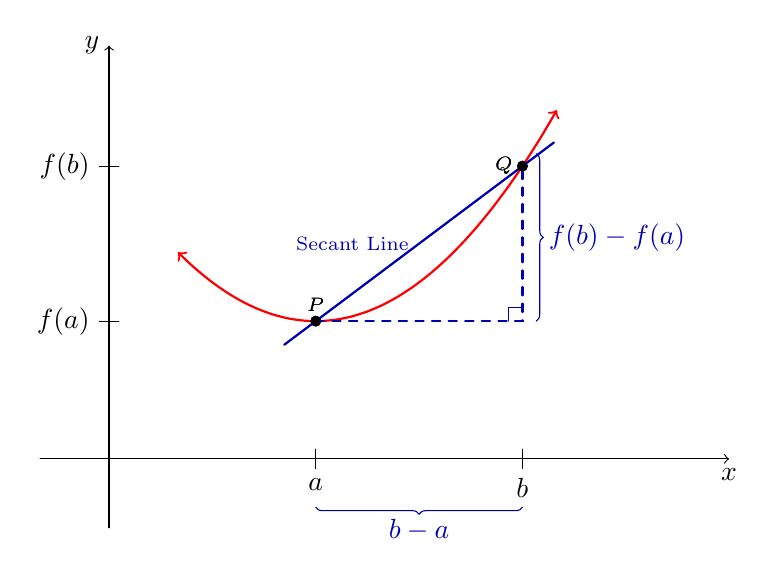
\begin{tikzpicture}[scale=1.75,cap=round]
\tikzset{axes/.style={}}
%\draw[style=help lines,step=1cm, dotted] (-5.25,-5.25) grid (5.25,5.25);
% The graphic
\begin{scope}[style=axes]
\draw[->] (-.5,0) -- (4.5,0) node[below] {$x$};
\draw[->] (0,-.5)-- (0,3) node[left] {$y$};
\foreach \x/\xtext in {1.5/a, 3/b}
 \draw[xshift=\x cm] (0pt,2pt) -- (0pt,-2pt) 
node[below,fill=white,font=\normalsize]
  {$\xtext$};    
\foreach \y/\ytext in {1/f(a), 2.125/f(b)}
  \draw[yshift=\y cm] (2pt,0pt) -- (-2pt,0pt) 
  node[left,fill=white,font=\normalsize]
  {$\ytext$};
  %%%
 \draw[domain=.5:3.25,smooth,variable=\x,red,<->,thick] plot ({\x},{.5*(\x-1.5)*(\x-1.5)+1});
  %%%
\filldraw[black] (1.5,1) circle (1pt) node[above] {\scriptsize $P$};
\filldraw[black] (3,2.125) circle (1pt) node[left] {\scriptsize $Q$};
\draw[thick,blue!70!black,shorten >=-.5cm,shorten <=-.5cm] (1.5,1)--(3,2.125) 
node[midway,left] {\scriptsize Secant Line};
 %%%
 \draw[blue!70!black,thick,dashed] (1.5,1)--(3,1)--(3,2.125);
 \draw[blue!70!black] (3,1.1)--(2.9,1.1)--(2.9,1);
 \draw[decoration={brace,mirror,raise=5pt},decorate,blue!70!black]
    (1.5,-.250) -- node[below=6pt] {$b-a$} (3,-.250);
 \draw[decoration={brace,mirror, raise=5pt},decorate,blue!70!black]
    (3,1) -- node[right=6pt] {$f(b)-f(a)$} (3,2.215);
 %%%
\filldraw[black] (1.5,1) circle (1pt) node[above] {\scriptsize $P$};
\filldraw[black] (3,2.125) circle (1pt) node[left] {\scriptsize $Q$};
\end{scope}
\end{tikzpicture}
\caption{\textit{A secant line threading two points along a curve \(f(x)\).}}
\end{center}
\end{figure}


\item \textbf{Instantaneous Rate of Change (IROC)}:
While AROC provides an average, we often seek to know how fast the function is changing at a specific point. The IROC at a point \( x = a \) is the derivative of the function, calculated as the limit of the AROC as the interval becomes infinitesimally small.

\item \textbf{Definition of the Derivative (Single Variable)}:
For a function \( f(x) \), the derivative at a point \( x = a \) is defined by the limit:
\[
f'(a) = \lim_{h \to 0} \frac{f(a + h) - f(a)}{h}
\]
This expression represents the slope of the tangent line to \( f \) at the point \( (a, f(a)) \), capturing the instantaneous rate of change of \( f(x) \) with respect to \( x \) at \( a \).


\begin{figure}[H]
\begin{center}
\begin{tikzpicture}[scale=1.75,cap=round]
\tikzset{axes/.style={}}
%\draw[style=help lines,step=1cm, dotted] (-5.25,-5.25) grid (5.25,5.25);
% The graphic
\begin{scope}[style=axes]
\draw[->] (-.5,0) -- (4.5,0) node[below] {$x$};
\draw[->] (0,-.5)-- (0,3) node[left] {$y$};
\foreach \x/\xtext in {1.5/a}
 \draw[xshift=\x cm] (0pt,2pt) -- (0pt,-2pt) 
node[below,fill=white,font=\normalsize]
  {$\xtext$};    
\foreach \y/\ytext in {1/f(a)}
  \draw[yshift=\y cm] (2pt,0pt) -- (-2pt,0pt) 
  node[left,fill=white,font=\normalsize]
  {$\ytext$};
  %%%
 \draw[domain=.5:3.25,smooth,variable=\x,red,<->,thick] plot ({\x},{.5*(\x-1.5)*(\x-1.5)+1});
  %%%
\filldraw[black] (1.5,1) circle (1pt) node[above] {\scriptsize $P$};
% Draw tangent line at P (horizontal line)
\draw[thick,blue] (0.5,1) -- (2.5,1) 
node[midway,below=6pt] {\scriptsize \textbf{Tangent Line}};
 %%%
\end{scope}
\end{tikzpicture}
\caption{\textit{A tangent line threadinga point along a curve \(f(x)\).}}
\end{center}
\end{figure}


\item \textbf{Basic Derivative Rules}\index{Derivative Rules}
The following rules simplify the process of finding derivatives for common functions.

\begin{itemize}
\item \textbf{Power Rule}: If \( f(x) = x^n \), then
\[
f'(x) = nx^{n-1}
\]
\item \textbf{Exponential Rule}: If \( f(x) = e^x \), then
\[
f'(x) = e^x
\]
\item \textbf{Logarithmic Rule}: If \( f(x) = \ln(x) \), then
\[
f'(x) = \frac{1}{x}
\]
\item \textbf{Sine Rule}: If \( f(x) = \sin(x) \), then
\[
f'(x) = \cos(x)
\]
\item \textbf{Cosine Rule}: If \( f(x) = \cos(x) \), then
\[
f'(x) = -\sin(x)
\]
\end{itemize}

\item \textbf{Product and Quotient Rules}\index{Product Rule}\index{Quotient Rule}
When dealing with the derivatives of products or quotients of functions, we use these rules:

\begin{itemize}
\item \textbf{Product Rule}: If \( f(x) = u(x)v(x) \), then
\[
f'(x) = u'(x)v(x) + u(x)v'(x)
\]
\item \textbf{Quotient Rule}: If \( f(x) = \frac{u(x)}{v(x)} \), then
\[
f'(x) = \frac{u'(x)v(x) - u(x)v'(x)}{[v(x)]^2}
\]
\end{itemize}

\item \textbf{Chain Rule}\index{Chain Rule}
For composite functions, we use the Chain Rule:

If \( f(x) = g(h(x)) \), then
\[
f'(x) = g'(h(x)) \cdot h'(x)
\]
The Chain Rule is essential when differentiating functions nested within other functions, allowing us to find the derivative of more complex expressions.

\end{itemize}

\exampleline
\begin{example}
Use the limit definition of the derivative to find the derivative of the function \( f(x) = x^2 \).

\begin{solution}
The derivative of \( f(x) = x^2 \) at a point \( x \) can be found using the limit definition of the derivative:
\[
f'(x) = \lim_{h \to 0} \frac{f(x+h) - f(x)}{h}
\]
\begin{enumerate}
    \item Substitute \( f(x) = x^2 \) into the formula:
    \[
    f'(x) = \lim_{h \to 0} \frac{(x+h)^2 - x^2}{h}
    \]
    \item Expand \( (x+h)^2 \):
    \[
    f'(x) = \lim_{h \to 0} \frac{x^2 + 2xh + h^2 - x^2}{h}
    \]
    \item Simplify by canceling \( x^2 \) terms:
    \[
    f'(x) = \lim_{h \to 0} \frac{2xh + h^2}{h}
    \]
    \item Factor out \( h \) from the numerator:
    \[
    f'(x) = \lim_{h \to 0} \frac{h(2x + h)}{h}
    \]
    \item Cancel \( h \) in the numerator and denominator:
    \[
    f'(x) = \lim_{h \to 0} (2x + h)
    \]
    \item Take the limit as \( h \to 0 \):
    \[
    f'(x) = 2x
    \]
\end{enumerate}
\end{solution}
\end{example}

% Place a single blue line after the example
\exampleline


\subsubsection*{Integrals} \index{Integrals}

Integrals form a foundational concept in calculus, representing the accumulation of quantities and the area under a curve. Integrals have applications across mathematics and science, such as calculating area, volume, work, and in modeling the behavior of physical systems. The process of integration is often considered the reverse operation of differentiation, and it provides insights into quantities that are accumulated or summed continuously over intervals. In this section, we will explore the integral as a limit of finite sums (Riemann Sum), develop the concept of definite and indefinite integrals, and introduce several integration techniques. 

\begin{itemize}
\item \textbf{Indefinite Integral}:  \index{Indefinite Integrals}
The indefinite integral of a function \( f(x) \), also known as the antiderivative, is defined as:
\[
\int f(x) \, dx = F(x) + C
\]
where \( F'(x) = f(x) \) and \( C \) is the constant of integration. This represents the family of all antiderivatives of \( f(x) \), capturing the essence of the function’s accumulated effect.

\item \textbf{Definite Integral}: \index{Definite Integrals}
The definite integral of \( f(x) \) over the interval \([a, b]\) is defined as:
\[
\int_a^b f(x) \, dx = F(b) - F(a)
\]
where \( F(x) \) is any antiderivative of \( f(x) \). The definite integral represents the net area between the curve \( f(x) \) and the \( x \)-axis from \( x = a \) to \( x = b \), taking into account areas above and below the axis.

\item \textbf{Riemann Sum and the Integral as a Limit of Finite Sums}: \index{Riemann Sum}
The concept of integration can be understood through the Riemann Sum, which approximates the area under a curve by summing the areas of rectangles. As the number of rectangles increases (and their width decreases), the sum approaches the exact area under the curve.

For a function \( f(x) \) over \([a, b]\), we divide the interval into \( n \) subintervals, each of width \( \Delta x = \frac{b - a}{n} \). The Riemann sum is:
\[
\sum_{i=1}^n f(x_i^*) \Delta x
\]
where \( x_i^* \) is a sample point within each subinterval. The definite integral is defined as the limit of this sum as \( n \to \infty \):
\[
\int_a^b f(x) \, dx = \lim_{n \to \infty} \sum_{i=1}^n f(x_i^*) \Delta x
\]

\begin{figure}[H]
\begin{center}
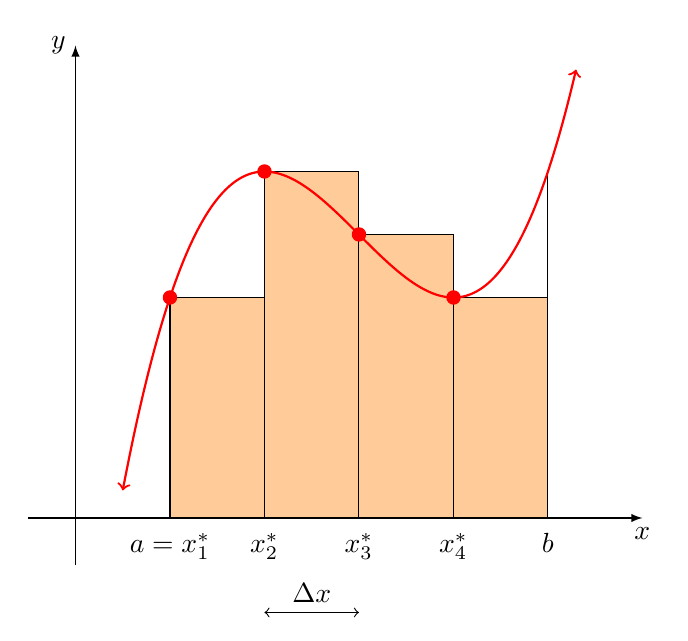
\begin{tikzpicture}[scale=1.2,declare function={f(\x)=((1/3)*(\x)^(3)-3*(\x)^(2)+8*\x-3;}]
\coordinate (start) at (.8,{f(.8)});
\coordinate (x0) at (1,{f(1)});
\coordinate (x1) at (2,{f(2)});
\coordinate (x2) at (3,{f(3)});
\coordinate (x3) at (4,{f(4)});
\coordinate (x4) at (5,{f(5)});
\coordinate (end) at (5.05,{f(5.05)});
\draw[fill=orange!40!white] (1,0) rectangle (2,{f(1)});
\draw[fill=orange!40!white] (2,0) rectangle (3,{f(2)});
\draw[fill=orange!40!white] (3,0) rectangle (4,{f(3)});
\draw[fill=orange!40!white] (4,0) rectangle (5,{f(4)});
\draw (5,0)--(5,{f(5)});
\draw [-latex] (-0.5,0) -- (6,0) node (xaxis) [below] {$x$};
\draw [-latex] (0,-0.5) -- (0,5) node [left] {$y$};
\foreach \x/\xtext in {1/a=x^*_{1} ,2/x^*_{2}, 3/x^*_{3} , 4/x^*_{4} , 5/b }
 \draw[xshift=\x cm] (0pt,3pt) -- (0pt,0pt) 
node[below=2pt,fill=white,font=\normalsize]
  {$\xtext$};
\draw[domain=.5:5.3,samples=200,variable=\x,red,<->,thick] plot ({\x},{f(\x)});                 
\foreach \n in {0,1,2,3}
\draw[red,fill=red] (x\n) circle (2pt) node[font=\normalsize] {$$};    
\draw[<->] (2,-1)--(3,-1) node[above,midway] {$\Delta x$};      
\end{tikzpicture}
\caption{\textit{A Riemann Sum approximation for an integral of a function.}}
\end{center}
\end{figure}

\index{Integral Approximations}
\item \textbf{Approximations Using Left, Right, and Center Points; Maxima, Minima, Supremum, and Infimum}: \index{Approximations in Riemann Sums}
Riemann sums allow for different choices of points within each subinterval to approximate the integral. These choices influence the accuracy and convergence of the sum, providing different approximations based on the choice of evaluation points within each subinterval.

\begin{itemize}
\item \textbf{Left Endpoint Approximation}: The function is evaluated at the left endpoint of each subinterval \( x_i \), producing a sum that may underestimate the area for increasing functions and overestimate for decreasing functions. The Riemann sum for \( n \) subintervals of width \( \Delta x = \frac{b - a}{n} \) is:
\[
\sum_{i=0}^{n-1} f(x_i) \, \Delta x
\]
where \( x_i = a + i \Delta x \) represents the left endpoint of each subinterval.

\item \textbf{Right Endpoint Approximation}: The function is evaluated at the right endpoint of each subinterval \( x_{i+1} \). This sum tends to overestimate for increasing functions and underestimate for decreasing functions:
\[
\sum_{i=1}^{n} f(x_{i+1}) \, \Delta x
\]
where \( x_i = a + i \Delta x \) represents the right endpoint of each subinterval.

\item \textbf{Midpoint (Center) Approximation}: The function is evaluated at the midpoint \( x_i^* = \frac{x_i + x_{i+1}}{2} \) of each subinterval. This approach often yields a more accurate approximation by balancing overestimates and underestimates:
\[
\sum_{i=0}^{n-1} f\left(x_i^*\right) \, \Delta x
\]
where \( x_i^* = a + \left(i + \frac{1}{2}\right) \Delta x \) is the midpoint.

\item \textbf{Maximal Approximation}: For each subinterval \( [x_i, x_{i+1}] \), choose the maximum function value, yielding an upper bound for the area:
\[
\sum_{i=0}^{n-1} \max_{x \in [x_i, x_{i+1}]} f(x) \, \Delta x
\]
This approximation gives an upper bound for the integral if \( f(x) \) is continuous over \([a, b]\).

\item \textbf{Minimal Approximation}: Similarly, choosing the minimum function value within each subinterval provides a lower bound:
\[
\sum_{i=0}^{n-1} \min_{x \in [x_i, x_{i+1}]} f(x) \, \Delta x
\]
This approximation serves as a lower bound if \( f(x) \) is continuous over \([a, b]\).

\item \textbf{Supremum and Infimum}: \index{Supremum and Infimum}
For theoretical purposes and cases with countably many discontinuous points, we can define Riemann sums using the supremum (least upper bound) and infimum (greatest lower bound) of \( f(x) \) on each subinterval, providing bounds as \( n \to \infty \). This approach is foundational in defining integrability:
\[
\sum_{i=0}^{n-1} \sup_{x \in [x_i, x_{i+1}]} f(x) \, \Delta x \quad \text{and} \quad \sum_{i=0}^{n-1} \inf_{x \in [x_i, x_{i+1}]} f(x) \, \Delta x
\]
These sums approximate the true integral more closely as \( n \to \infty \).
\end{itemize}

\item \textbf{Numerical Integration Techniques} \index{Numerical Integration}
When exact integration is challenging, numerical integration methods approximate the value of definite integrals by evaluating the function at specific points. Key methods include:
\begin{itemize}
\item \textbf{Trapezoidal Rule}: Approximates the area under the curve by dividing it into trapezoids rather than rectangles, averaging the left and right endpoint evaluations: \index{Trapezoidal Rule}
\[
\int_a^b f(x) \, dx \approx \frac{\Delta x}{2} \left[ f(x_0) + 2\sum_{i=1}^{n-1} f(x_i) + f(x_n) \right]
\]
where \( \Delta x = \frac{b - a}{n} \) and \( x_0, x_1, \dots, x_n \) are equally spaced points.

\item \textbf{Simpson's Rule}: \index{Simpson's Rule} Uses parabolic segments to approximate the curve. It is more accurate for functions that are reasonably smooth and is defined as:
\[
\int_a^b f(x) \, dx \approx \frac{\Delta x}{3} \left[ f(x_0) + 4\sum_{\text{odd } i} f(x_i) + 2\sum_{\text{even } i} f(x_i) + f(x_n) \right]
\]
\end{itemize}
Simpson’s Rule provides excellent accuracy for a modest number of intervals, especially for polynomials and smooth functions.


\exampleline
\begin{example}
Use Simpson's Rule with \( n = 4 \) subintervals to approximate the integral \( \int_0^{2} \frac{1}{1 + x^2} \, dx \). Compare the result with the exact value of the integral.

\begin{solution}
Since Simpson's Rule requires knowing the exact value to compare, we start by calculating the exact value of the integral:
\[
\int_0^{2} \frac{1}{1 + x^2} \, dx = \left[ \arctan x \right]_0^2 = \arctan 2 - \arctan 0 = \arctan 2.
\]

\begin{enumerate}
    \item Calculate the width of each subinterval:
    \[
    h = \frac{b - a}{n} = \frac{2 - 0}{4} = 0.5.
    \]

    \item Determine the \( x \)-values:
    \[
    x_0 = 0,\quad x_1 = 0.5,\quad x_2 = 1.0,\quad x_3 = 1.5,\quad x_4 = 2.0.
    \]

    \item Compute the corresponding \( y \)-values:
    \begin{align*}
    y_0 &= \frac{1}{1 + (0)^2} = 1, \\
    y_1 &= \frac{1}{1 + (0.5)^2} = \frac{1}{1.25} = 0.8, \\
    y_2 &= \frac{1}{1 + (1)^2} = \frac{1}{2} = 0.5, \\
    y_3 &= \frac{1}{1 + (1.5)^2} = \frac{1}{3.25} \approx 0.3077, \\
    y_4 &= \frac{1}{1 + (2)^2} = \frac{1}{5} = 0.2.
    \end{align*}

    \item Apply Simpson's Rule:
    \[
    \int_0^{2} \frac{1}{1 + x^2} \, dx \approx \frac{h}{3} \left( y_0 + 4y_1 + 2y_2 + 4y_3 + y_4 \right).
    \]
    Substitute the computed values:
    \[
    \int_0^{2} \frac{1}{1 + x^2} \, dx \approx \frac{0.5}{3} \left( 1 + 4(0.8) + 2(0.5) + 4(0.3077) + 0.2 \right).
    \]

    Calculate the expression inside the parentheses:
    \begin{align*}
    &1 + 4(0.8) + 2(0.5) + 4(0.3077) + 0.2 \\
    &= 1 + 3.2 + 1.0 + 1.2308 + 0.2 \\
    &= 6.6308.
    \end{align*}

    Compute the approximation:
    \[
    \int_0^{2} \frac{1}{1 + x^2} \, dx \approx \frac{0.5}{3} \times 6.6308 = \frac{3.3154}{3} \approx 1.1051.
    \]

    \item Compare with the exact value:
    \[
    \arctan 2 \approx 1.1071.
    \]
\end{enumerate}

The Simpson's Rule approximation is \( 1.1051 \), while the exact value is approximately \( 1.1071 \). The error is approximately \( 0.0020 \).
\end{solution}
\end{example}
\exampleline

\item \textbf{Basic Integrals}\index{Basic Integral Formulas}:
Several integral rules and formulas are essential for computing integrals efficiently. Here are some fundamental examples:

\begin{itemize}
\item \textbf{Power Rule}: For \( n \neq -1 \),
\[
\int x^n \, dx = \frac{x^{n+1}}{n+1} + C
\]
\item \textbf{Logarithmic Rule}:
\[
\int \frac{1}{x} \, dx = \ln|x| + C
\]
\item \textbf{Exponential Rule}:
\[
\int e^x \, dx = e^x + C
\]
\item \textbf{Sine Rule}:
\[
\int \sin(x) \, dx = -\cos(x) + C
\]
\item \textbf{Cosine Rule}:
\[
\int \cos(x) \, dx = \sin(x) + C
\]
\end{itemize}

\item \textbf{Integration by Parts}: \index{Integration by Parts}
This technique is useful when integrating products of functions. It is derived from the product rule for differentiation and is given by:
\[
\int u \, dv = uv - \int v \, du
\]





\item \textbf{DI Method (Tabular Method)}: \index{Tabular Method}
To evaluate integrals using the DI method, construct a table with three columns: Sign, $D$, and $I$. Differentiate the function that simplifies upon differentiation (usually $u$) and integrate the function that does not change much upon integration (usually $dv$). This method is particularly useful in solving Partial Differential Equations (PDEs) because it systematically reduces the complexity of integrals involving products of functions, making it easier to handle boundary conditions and find solutions. \\ \\ The objective is to continue differentiating in the $D$ column until reaching 0. For each row, you multiply diagonally from the $D$ term to the $I$ term, following the specified sign. You can choose to stop early and integrate the last row separately if a pattern allows. Once the $D$ column reaches zero, any further terms contribute nothing to the integral. We have color coded and marked with asterisks the terms in the table to add together.

\vspace{1em}
\begin{center}
\begin{tabular}{|c|c|c|}
\hline
Sign & $D$ & $I$ \\
\hline
$+$ & \textcolor{blue}{$u$ (*)} & {$dv$} \\
$-$ & \textcolor{red}{$u'$ (**) } & \textcolor{blue}{$\int dv$ (*) } \\
$+$ & \textcolor{purple}{$u''$ (***)} & \textcolor{red}{$\int \left(\int dv\right) dv $ (**)} \\
$-$ & {$u'''$} & \textcolor{purple}{$\int \left(\int \left(\int dv\right) dv \right) dv$ (***)} \\
\hline
\end{tabular}
\end{center}
\begin{center}
\textit{Note: Integrate here for the last term.}
\end{center}

The integral is computed by summing the diagonal products, following the pattern until the final term reaches zero.





\vspace{1em}
\item \textbf{Substitution Method}: \index{Substitution Method}
Also known as \( u \)-substitution, this method is helpful for integrals involving compositions of functions. If \( u = g(x) \), then
\[
\int f(g(x)) g'(x) \, dx = \int f(u) \, du
\]


\item \textbf{Definite Integral Evaluation Using the Fundamental Theorem of Calculus}:
The Fundamental Theorem of Calculus links differentiation and integration, stating that if \( F \) is an antiderivative of \( f \) on \([a, b]\), then:
\[
\int_a^b f(x) \, dx = F(b) - F(a)
\]
This theorem provides a way to evaluate the exact area under a curve using antiderivatives.

\end{itemize}


\exampleline
\begin{example}
Evaluate \( \int x^3 e^x \, dx \) using the DI (Tabular) Method.

\begin{solution}
We’ll apply the DI method, choosing \( x^3 \) to differentiate and \( e^x \) to integrate. Construct the table as follows:

\vspace{1em}
\begin{center}
\begin{tabular}{|c|c|c|}
\hline
Sign & $D$ & $I$ \\
\hline
+ & $x^3$ & $e^x$ \\
- & $3x^2$ & $e^x$ \\
+ & $6x$ & $e^x$ \\
- & $6$ & $e^x$ \\
+ & $0$ & $e^x$ \\
\hline
\end{tabular}
\end{center}
\vspace{1em}

\noindent Now, we combine terms according to the DI method by multiplying entries across each row (taking the signs into account) and summing the results:

\[
\int x^3 e^x \, dx = x^3 e^x - 3x^2 e^x + 6x e^x - 6 e^x + C
\]
\end{solution}
\end{example}
\exampleline




\subsubsection*{Other Useful Integration Rules} \index{Integration Rules}

In addition to basic integration techniques, there are several advanced methods that help solve more complex integrals. These methods expand the range of integrals we can compute by breaking down complex functions into simpler parts, leveraging trigonometric identities, or applying specific substitutions.

\begin{itemize}
\item \textbf{Integration by Partial Fractions}: \index{Partial Fractions}
Partial fraction decomposition is useful for integrating rational functions (ratios of polynomials). This technique involves breaking a complicated rational function into a sum of simpler fractions that can be integrated individually.

    \begin{itemize}
    \item \textbf{Steps for Partial Fraction Decomposition}:
        \begin{enumerate}
        \item Factor the denominator, if possible.
        \item Write the integrand as a sum of partial fractions. For example, if the denominator factors as \( (x - a)(x - b) \), write:
            \[
            \frac{P(x)}{(x - a)(x - b)} = \frac{A}{x - a} + \frac{B}{x - b}
            \]
        \item Solve for the constants (\( A \), \( B \), etc.) by equating coefficients or substituting convenient values for \( x \).
        \item Integrate each term separately.
        \end{enumerate}


    \end{itemize}

\item \textbf{Trigonometric Integrals}: \index{Trigonometric Integrals}
Trigonometric integrals involve expressions with trigonometric functions, such as \( \sin^n(x) \), \( \cos^m(x) \), or combinations like \( \sin(x) \cos(x) \). Simplifying these integrals often requires trigonometric identities.

    \begin{itemize}
    \item \textbf{Key Identities for Simplification}:
        \begin{itemize}
        \item \( \sin^2(x) = \frac{1 - \cos(2x)}{2} \)
        \item \( \cos^2(x) = \frac{1 + \cos(2x)}{2} \)
        \item \( \sin(x)\cos(x) = \frac{\sin(2x)}{2} \)
        \end{itemize}

    \end{itemize}

\item \textbf{Trigonometric Substitution}: \index{Trigonometric Substitution}
Trigonometric substitution is useful for integrating expressions containing square roots, such as \( \sqrt{a^2 - x^2} \), \( \sqrt{a^2 + x^2} \), or \( \sqrt{x^2 - a^2} \). By making a substitution involving trigonometric functions, we can transform these integrals into simpler forms.

    \begin{itemize}
    \item \textbf{Common Substitutions}:
\vspace{1em}
        \begin{center}
        \begin{tabular}{|c|c|c|}
        \hline
        Expression & Substitution & Resulting Identity \\
        \hline
        \( \sqrt{a^2 - x^2} \) & \( x = a \sin(\theta) \) & \( \sqrt{a^2 - x^2} = a \cos(\theta) \) \\
        \( \sqrt{a^2 + x^2} \) & \( x = a \tan(\theta) \) & \( \sqrt{a^2 + x^2} = a \sec(\theta) \) \\
        \( \sqrt{x^2 - a^2} \) & \( x = a \sec(\theta) \) & \( \sqrt{x^2 - a^2} = a \tan(\theta) \) \\
        \hline
        \end{tabular}
        \end{center}
\vspace{1em}
    \end{itemize}

\item \textbf{Reduction Formulas}: \index{Reduction Formulas}
Reduction formulas provide a recursive way to evaluate integrals of certain functions, often involving powers of trigonometric functions or products of functions. These formulas allow us to reduce the power of the integrand step-by-step, eventually reaching a simpler integral.

    \begin{itemize}
    \item \textbf{Example of a Reduction Formula for Powers of Sine}:
        \[
        \int \sin^n(x) \, dx = -\frac{\sin^{n-1}(x) \cos(x)}{n} + \frac{n-1}{n} \int \sin^{n-2}(x) \, dx
        \]
    \end{itemize}
\end{itemize}

\subsubsection*{Taylor Series} \index{Taylor Series}

Taylor Series provide a way to approximate functions using polynomials, which can make complex functions easier to work with in calculus, physics, engineering, and beyond. This series expansion allows us to approximate functions locally around a point by using the derivatives of the function at that point. 

\begin{itemize}
\item \textbf{Definition}:
For a function \( f(x) \) that is infinitely differentiable at \( a \), the Taylor series expansion of \( f(x) \) around \( x = a \) is:
\[
f(x) = f(a) + f'(a)(x-a) + \frac{f''(a)}{2!}(x-a)^2 + \frac{f'''(a)}{3!}(x-a)^3 + \cdots
\]
or, in summation notation:
\[
f(x) = \sum_{n=0}^{\infty} \frac{f^{(n)}(a)}{n!} (x-a)^n
\]
This expansion allows us to represent \( f(x) \) as an infinite series of terms involving powers of \( (x - a) \), with each term weighted by the function's \( n \)-th derivative evaluated at \( a \). The closer \( x \) is to \( a \), the better the approximation.

\item \textbf{Maclaurin Series}: \index{Maclaurin Series}
A Maclaurin series is a special case of the Taylor series centered at \( a = 0 \):
\[
f(x) = f(0) + f'(0)x + \frac{f''(0)}{2!}x^2 + \frac{f'''(0)}{3!}x^3 + \cdots = \sum_{n=0}^{\infty} \frac{f^{(n)}(0)}{n!} x^n
\]
Maclaurin series are commonly used for standard functions such as \( e^x \), \( \sin(x) \), and \( \cos(x) \).

\item \textbf{Common Maclaurin Series Expansions}:

These series expansions provide useful approximations for frequently encountered functions:

    \begin{itemize}
    \item \textbf{Exponential Function} \( e^x \):
        \[
        e^x = 1 + x + \frac{x^2}{2!} + \frac{x^3}{3!} + \cdots = \sum_{n=0}^{\infty} \frac{x^n}{n!}
        \]
        The exponential function \( e^x \) is unique in that it is its own derivative and its own Taylor series, making it fundamental in calculus.

    \item \textbf{Sine Function} \( \sin(x) \):
        \[
        \sin(x) = x - \frac{x^3}{3!} + \frac{x^5}{5!} - \cdots = \sum_{n=0}^{\infty} (-1)^n \frac{x^{2n+1}}{(2n+1)!}
        \]
        This series shows the odd power expansion of \( \sin(x) \), alternating in sign. It is especially useful in approximations for small \( x \), where only a few terms may be needed.

    \item \textbf{Cosine Function} \( \cos(x) \):
        \[
        \cos(x) = 1 - \frac{x^2}{2!} + \frac{x^4}{4!} - \cdots = \sum_{n=0}^{\infty} (-1)^n \frac{x^{2n}}{(2n)!}
        \]
        Similar to the sine series, the cosine function’s Maclaurin series consists of even powers of \( x \), with alternating signs. This series provides an accurate approximation for \( \cos(x) \) near \( x = 0 \).

    \item \textbf{Logarithmic Function} \( \ln(1 + x) \) (valid for \( -1 < x \leq 1 \)):
        \[
        \ln(1 + x) = x - \frac{x^2}{2} + \frac{x^3}{3} - \frac{x^4}{4} + \cdots = \sum_{n=1}^{\infty} (-1)^{n+1} \frac{x^n}{n}
        \]
        This series is useful in approximating logarithmic functions around \( x = 0 \).

    \item \textbf{Arc Tangent Function} \( \arctan(x) \) (valid for \( -1 \leq x \leq 1 \)):
        \[
        \arctan(x) = x - \frac{x^3}{3} + \frac{x^5}{5} - \cdots = \sum_{n=0}^{\infty} (-1)^n \frac{x^{2n+1}}{2n+1}
        \]
        This series provides an approximation for the inverse tangent function near \( x = 0 \), often useful in trigonometric applications.

    \end{itemize}

\item \textbf{Remainder Term and Approximation Accuracy}:
When using Taylor or Maclaurin series to approximate functions, it is important to understand the error or remainder involved in truncating the series. For a Taylor series approximation up to the \( n \)-th term, the remainder \( R_n(x) \) gives the difference between the actual function and the Taylor polynomial.

    \[
    R_n(x) = \frac{f^{(n+1)}(c)}{(n+1)!} (x-a)^{n+1} \text{ for some } c \text{ between } a \text{ and } x
    \]
This remainder term shows how the accuracy of the approximation depends on the higher derivatives of \( f(x) \), the point \( x \), and the number of terms included in the approximation.

\end{itemize}

\exampleline
\begin{example}
Find the Taylor series of \( f(x) = \ln(1+x) \) centered at \( a=0 \) up to the third term.

\begin{solution}
To find the Taylor series, we calculate the derivatives of \( f(x) \) at \( x=0 \) and use them to construct the series.

\begin{enumerate}
    \item Calculate \( f(x) \) and its derivatives:
    \begin{align*}
    f(x) &= \ln(1+x) \\
    f'(x) &= \frac{1}{1+x} \\
    f''(x) &= -\frac{1}{(1+x)^2} \\
    f'''(x) &= \frac{2}{(1+x)^3}
    \end{align*}

    \item Evaluate these derivatives at \( x=0 \):
    \begin{align*}
    f(0) &= \ln(1) = 0 \\
    f'(0) &= 1 \\
    f''(0) &= -1 \\
    f'''(0) &= 2
    \end{align*}

    \item Use the Taylor series formula up to the third term:
    \[
    f(x) \approx f(0) + f'(0)(x) + \frac{f''(0)}{2!}x^2 + \frac{f'''(0)}{3!}x^3
    \]

    \item Substitute the values:
    \[
    f(x) \approx 0 + x - \frac{1}{2}x^2 + \frac{1}{3}x^3
    \]
\end{enumerate}
\end{solution}
\end{example}
\exampleline


\subsection*{Important Theorems and Results in Calculus} 

\noindent Understanding key theorems in calculus is crucial for solving ordinary differential equations (ODEs), as these results often provide the foundation for methods of integration, approximation, and analysis. They help in determining the behavior of solutions, establishing existence and uniqueness, and transforming complex problems into more manageable forms. Here are some of the most significant theorems:

\begin{itemize}

\item \textbf{Mean Value Theorem (MVT)}:  \index{Mean Value Theorem}
If \( f(x) \) is continuous on \( [a,b] \) and differentiable on \( (a,b) \), then there exists a point \( c \) in \( (a,b) \) such that:
$$f'(c) = \frac{f(b) - f(a)}{b - a}$$
This theorem asserts that for a smooth curve between \( a \) and \( b \), there is at least one point where the tangent (instantaneous rate of change) is parallel to the secant line connecting \( (a, f(a)) \) and \( (b, f(b)) \).

\item \textbf{Rolle's Theorem}:  \index{Rolle's Theorem}
If \( f(x) \) is continuous on \( [a,b] \), differentiable on \( (a,b) \), and \( f(a) = f(b) \), then there exists a point \( c \) in \( (a,b) \) such that \( f'(c) = 0 \).
This theorem is a special case of the MVT, asserting that if a function returns to the same value at two points, there must be at least one point in between where the derivative (slope of the tangent) is zero.

\item \textbf{Intermediate Value Theorem (IVT)}:  \index{Intermediate Value Theorem}
If \( f(x) \) is continuous on \( [a,b] \) and \( k \) is any value between \( f(a) \) and \( f(b) \), then there exists a point \( c \) in \( [a,b] \) such that \( f(c) = k \).
The IVT guarantees that a continuous function takes on every intermediate value between \( f(a) \) and \( f(b) \), a property crucial for establishing the existence of solutions.

\item \textbf{Extreme Value Theorem (EVT)}:  \index{Extreme Value Theorem}
If \( f(x) \) is continuous on a closed interval \( [a,b] \), then \( f \) attains both a maximum and a minimum value on \( [a,b] \).
This theorem ensures that a continuous function over a closed interval has both an absolute maximum and minimum, critical for optimization problems and boundary analyses.

\item \textbf{L'Hôpital's Rule}:  \index{L'Hôpital's Rule}
If \( \lim_{x \to a} \frac{f(x)}{g(x)} \) results in the indeterminate form \( \frac{0}{0} \) or \( \frac{\infty}{\infty} \), then:
$$\lim_{x \to a} \frac{f(x)}{g(x)} = \lim_{x \to a} \frac{f'(x)}{g'(x)}$$
provided the limit on the right exists or is infinite. This rule is essential for evaluating limits that yield indeterminate forms, often encountered in calculus and differential equations.

\item \textbf{First Fundamental Theorem of Calculus (FTOC I)}: \index{Fundamental Theorem of Calculus}
If \( f \) is continuous on \( [a, b] \) and \( F \) is an antiderivative of \( f \) on \( [a, b] \), then:
$$\int_a^b f(x) \, dx = F(b) - F(a)$$
This theorem links the process of differentiation and integration, showing that the definite integral of a function over an interval can be computed using any of its antiderivatives.

\item \textbf{Second Fundamental Theorem of Calculus (FTOC II)}: \index{Fundamental Theorem of Calculus}
If \( f \) is continuous on an interval containing \( a \), then for any \( x \) in that interval:
$$\frac{d}{dx} \int_a^x f(t) \, dt = f(x)$$
This theorem states that the derivative of the integral function (accumulated area) is the original function, demonstrating how integration can "undo" differentiation.

\item \textbf{Leibniz Rule for Differentiation under the Integral Sign}: \index{Leibniz Rule}
If \( f(x, t) \) is continuous on \( x \) and \( t \), and \( \partial f / \partial t \) exists and is continuous, then:
$$\frac{d}{dx} \int_{a(x)}^{b(x)} f(x, t) \, dt = f(x, b(x)) \cdot \frac{db}{dx} - f(x, a(x)) \cdot \frac{da}{dx} + \int_{a(x)}^{b(x)} \frac{\partial}{\partial x} f(x, t) \, dt$$
This rule is crucial in scenarios where integration limits depend on \( x \), enabling differentiation within the integral sign.

\item \textbf{Taylor’s Theorem} \index{Taylor's Theorem}
For a function \( f(x) \) that is \( n+1 \)-times differentiable at \( a \), Taylor’s Theorem gives an approximation for \( f(x) \) near \( a \):
$$f(x) = f(a) + f'(a)(x-a) + \frac{f''(a)}{2!}(x-a)^2 + \cdots + \frac{f^{(n)}(a)}{n!}(x-a)^n + R_n(x)$$
where \( R_n(x) \) is the remainder term. In the limit as \( n \to \infty \), if \( R_n(x) \to 0 \), we obtain the Taylor Series:
$$f(x) = \sum_{k=0}^{\infty} \frac{f^{(k)}(a)}{k!} (x-a)^k$$
Taylor's Theorem is fundamental in approximating functions locally using polynomials and is widely applied in numerical analysis and differential equations.


\end{itemize}


\exampleline
\begin{example}
Verify that the function \( f(x) = x^2 - 3x + 2 \) satisfies the Mean Value Theorem on the interval \([1, 4]\), and find the value of \( c \) that satisfies the theorem.

\begin{solution}
To apply the Mean Value Theorem (MVT), we need to confirm that \( f(x) \) is continuous on \([1, 4]\) and differentiable on \((1, 4)\). Since \( f(x) = x^2 - 3x + 2 \) is a polynomial, it is continuous and differentiable everywhere, so the MVT applies on this interval. According to the Mean Value Theorem, there exists a point \( c \in (1, 4) \) such that:
\[
f'(c) = \frac{f(4) - f(1)}{4 - 1}
\]

\begin{enumerate}
    \item Calculate \( f(4) \) and \( f(1) \):
    \begin{align*}
    f(4) &= 4^2 - 3 \cdot 4 + 2 = 16 - 12 + 2 = 6 \\
    f(1) &= 1^2 - 3 \cdot 1 + 2 = 1 - 3 + 2 = 0
    \end{align*}

    \item Compute the average rate of change:
    \[
    \frac{f(4) - f(1)}{4 - 1} = \frac{6 - 0}{3} = 2
    \]

    \item Differentiate \( f(x) \) and set \( f'(c) = 2 \):
    \[
    f'(x) = 2x - 3
    \]
    Setting \( f'(c) = 2 \), we get:
    \[
    2c - 3 = 2
    \]
    Solving for \( c \):
    \[
    2c = 5 \Rightarrow c = \frac{5}{2} = 2.5
    \]

    \item Verify \( c \in (1, 4) \):
    Since \( c = 2.5 \) lies within the interval \((1, 4)\), it satisfies the conditions of the Mean Value Theorem.
\end{enumerate}

\end{solution}
\end{example}
\exampleline

\newpage


\lecture{Three-Dimensional Coordinate Systems} \index{Coordinate Systems}

\noindent Transitioning from two-dimensional to three-dimensional coordinate systems marks a significant leap in our capacity to represent and analyze objects and interactions spatially. This shift extends our geometric understanding, equipping us with a powerful framework for calculating points, distances, and angles within three-dimensional space—a foundational requirement for advanced calculus, physics, engineering, and numerous other fields.

\subsection*{Rectangular Coordinates in Two Dimensions} \index{Rectangular Coordinates}

In two dimensions, every point on a plane is specified by a coordinate pair, \( (x, y) \), where \( x \) and \( y \) represent distances along two mutually perpendicular axes: the \( x \)-axis (horizontal) and \( y \)-axis (vertical). This two-dimensional system is essential for understanding how we map points in a flat plane and serves as a stepping stone for more complex spatial reasoning. In a 2D Cartesian system, an ordered pair \( (x, y) \) not only specifies location but also allows us to measure distances, areas, and angular relationships on a flat plane.

\begin{figure}[H]
    \centering
    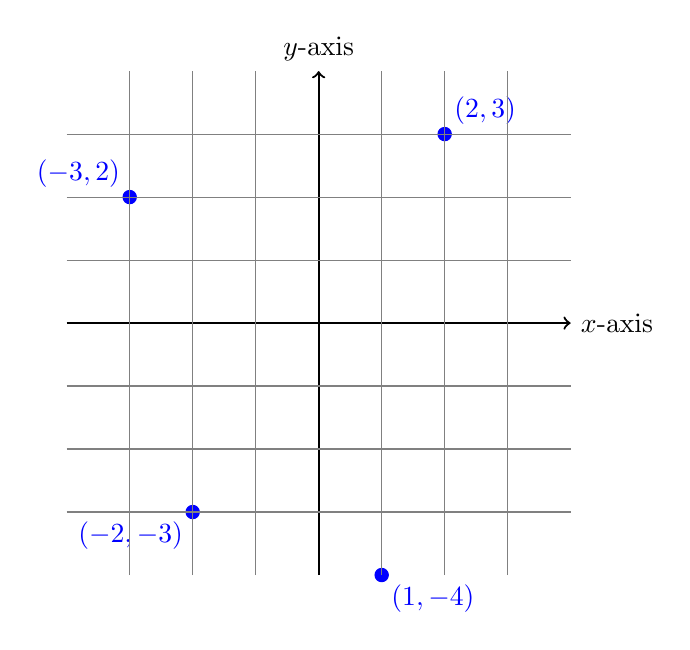
\begin{tikzpicture}[scale=0.8]
        % Draw axes
        \draw[thick,->] (-4, 0) -- (4, 0) node[right] {$x$-axis};
        \draw[thick,->] (0, -4) -- (0, 4) node[above] {$y$-axis};

        % Points on the plane
        \filldraw[blue] (2, 3) circle (3pt) node[anchor=south west] {$(2, 3)$};
        \filldraw[blue] (-3, 2) circle (3pt) node[anchor=south east] {$(-3, 2)$};
        \filldraw[blue] (1, -4) circle (3pt) node[anchor=north west] {$(1, -4)$};
        \filldraw[blue] (-2, -3) circle (3pt) node[anchor=north east] {$(-2, -3)$};

        % Grid
        \foreach \x in {-3,-2,-1,1,2,3}
            \draw[gray, thin] (\x, -4) -- (\x, 4);
        \foreach \y in {-3,-2,-1,1,2,3}
            \draw[gray, thin] (-4, \y) -- (4, \y);
    \end{tikzpicture}
    \caption{\textit{2D Cartesian Coordinate System showing points such as \((2, 3)\) and \((-3, 2)\)}}
    \label{fig:2d_cartesian}
\end{figure}

\subsection*{Introduction to Three-Dimensional Space}

\noindent By introducing a third axis, the \( z \)-axis, we can move into three-dimensional space, where each point is described by an ordered triple \( (x, y, z) \). The addition of the \( z \)-axis—perpendicular to both \( x \) and \( y \)—allows us to locate points and measure distances not only horizontally and vertically but also in terms of depth or height. This extension from two to three dimensions mirrors our physical world and enables us to mathematically describe real objects, from simple geometric shapes to complex structures. \\ 

\noindent In three-dimensional space:
\begin{itemize}
\item \( x \): Measures the position along the \( x \)-axis (typically horizontal).
\item \( y \): Measures the position along the \( y \)-axis (perpendicular to the \( x \)-axis).
\item \( z \): Measures the position along the \( z \)-axis (perpendicular to both \( x \) and \( y \) axes).
\end{itemize}

\noindent This system allows us to define planes formed by pairs of axes:
\begin{itemize}
\item \textit{The \( xy \)-plane}, where \( z = 0 \), represents a flat surface in the horizontal and vertical dimensions. This is the familiar coordinate plane from previous mathematics courses.
\item \textit{The \( xz \)-plane}, where \( y = 0 \), represents a plane incorporating depth along \( z \) and position along \( x \). This plane would appear as a vertical wall if you were looking directly at it.
\item \textit{The \( yz \)-plane}, where \( x = 0 \), allows us to represent depth along \( z \) and height along \( y \). This too appears as a vertical wall, but perpendicular to the \( xz \)-plane.
\end{itemize}

\noindent These three coordinate planes divide space into eight regions called octants, with the first octant being where all coordinates are positive. This organization helps us understand spatial relationships and serves as the foundation for our study of multivariable calculus. Throughout this course, we will learn to analyze functions, curves, and surfaces in this three-dimensional setting, building upon our knowledge of calculus in one and two dimensions. \\

\noindent When visualizing three-dimensional objects, we often use perspective drawings where parallel lines appear to meet at a distance. This technique helps us represent three-dimensional concepts on a two-dimensional page while maintaining our intuitive understanding of spatial relationships.

\begin{figure}[H]
\centering
\begin{tikzpicture}
\begin{axis}[
colormap/PuOr,
grid=major,
xlabel={$x$-axis},
ylabel={$y$-axis},
zlabel={$z$-axis},
scaled ticks=false
]
\addplot3+ [
mesh,
scatter,
samples=10,
domain=0:1,
] {x*(1-x)*y*(1-y)};
\end{axis}
\end{tikzpicture}

\caption{\textit{3D Cartesian Coordinate System with sample points in space connected by lines.}}
\label{fig:3d_cartesian}
\end{figure}

\noindent The intersection of these planes at the origin divides space into eight distinct regions, called octants. We locate any point \( (x, y, z) \) by moving \( x \) units along the \( x \)-axis, \( y \) units along the \( y \)-axis, and \( z \) units along the \( z \)-axis. This spatial representation is fundamental in fields like navigation, robotics, and physics, where understanding three dimensions is critical to applications ranging from satellite positioning to structural analysis.
%https://commons.wikimedia.org/wiki/File:Octant_numbers.svg
\begin{figure}[H]
\centering
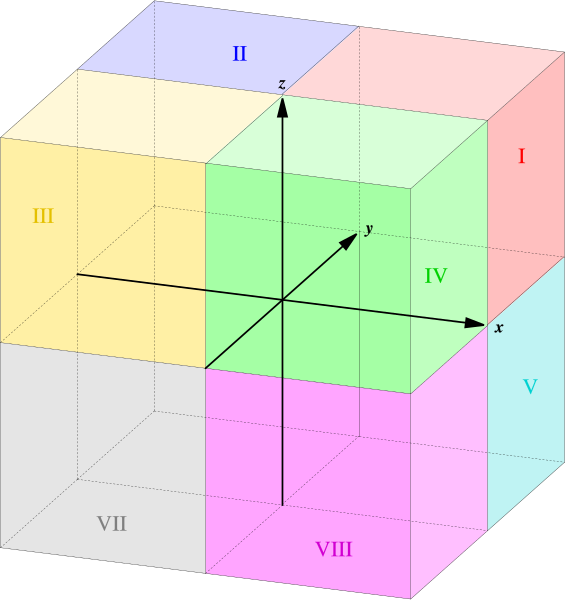
\includegraphics[width=0.4\textwidth]{chapters/chp1_pics/octant.png}
\caption{\textit{The eight octants of a three-dimensional Cartesian plot.}}
\label{fig:steinmetz}
\end{figure}

\subsection*{Toward Higher Dimensions: Imagining Four-Dimensional Space}

\noindent Extending to a fourth spatial dimension—though challenging to visualize—invites us to think beyond our physical intuition. In a four-dimensional space, each point is represented by an ordered quadruple \( (x, y, z, w) \), where \( w \) denotes the fourth dimension. Though difficult to imagine, one can think of \( w \) as adding an additional degree of freedom beyond our typical three-dimensional experience. Mathematicians and physicists work in four-dimensional (and higher-dimensional) spaces when dealing with complex phenomena, such as in the study of spacetime in general relativity. \\ \\ A helpful analogy is to consider how three-dimensional objects can cast two-dimensional shadows. In the same way, a four-dimensional object, known as a tesseract or hypercube, could project a three-dimensional “shadow.” This shadow could show us a trace of four-dimensional interactions, allowing us to infer properties of the higher dimension. While our intuition may falter beyond three dimensions, mathematical models provide structure. Calculations in higher-dimensional spaces can help solve problems in fields such as quantum mechanics and data science, where multi-dimensional datasets reveal patterns not visible in lower dimensions.





\subsection*{Distance and Midpoint Formulas in Three Dimensions} \index{Metric Formulas}

The distance and midpoint formulas in three-dimensional space are extensions of the two-dimensional formulas, derived from the Pythagorean Theorem. By understanding these derivations, we gain insight into the geometry of space and the relationships between points in three dimensions.

\subsubsection*{Derivation of the Distance Formula}

The distance formula in geometry is a direct extension of the Pythagorean Theorem, which states that for a right triangle with legs \( a \) and \( b \), and hypotenuse \( c \), the relationship between the sides is $a^2 + b^2 = c^2.$ We rearrange this equation for the hypotenuse to get $c = \sqrt{a^2 + b^2}$ This formula gives the length of the hypotenuse when the lengths of the other two sides are known. Now, consider finding the distance between two points \( P_1(x_1, y_1) \) and \( P_2(x_2, y_2) \) in a two-dimensional plane. To derive this distance, we construct a right triangle by taking the horizontal and vertical distances between these points:
\[
a = x_2 - x_1 \quad \text{and} \quad b = y_2 - y_1.
\]

\noindent Substituting \( a \) and \( b \) into the Pythagorean Theorem, we get:
\[
(x_2 - x_1)^2 + (y_2 - y_1)^2 = d^2,
\]
where \( d \) represents the distance between \( P_1 \) and \( P_2 \). Solving for \( d \) gives us the two-dimensional distance formula:
\[
d = \sqrt{(x_2 - x_1)^2 + (y_2 - y_1)^2}.
\]

\subsubsection*{Extending the Distance Formula to Three Dimensions}

To generalize this result to three-dimensional space, we need to consider an additional dimension, the \( z \)-axis. Given two points \( P_1(x_1, y_1, z_1) \) and \( P_2(x_2, y_2, z_2) \), the change in the \( z \)-direction introduces an additional ``side” in the Pythagorean relationship. Now, we have three differences:
\[
a = x_2 - x_1, \quad b = y_2 - y_1, \quad \text{and} \quad c = z_2 - z_1.
\]
\noindent We follow the same logic as before to obtain
\[
d = \sqrt{(x_2 - x_1)^2 + (y_2 - y_1)^2 + (z_2 - z_1)^2}.
\]

\noindent This formula allows us to calculate the straight-line distance between any two points in three-dimensional space by considering the differences along each of the three axes. Notice, that because of the square terms, the distance will always be positive or zero. Since we saw that for the Pythagorean theorem all we had to do to increase the dimensionality was include one more square term,  let's do that $n$-many times to go to any $n$th dimension we desire. Thus we obtain for any $n$-dimension we have
\[
d = \left(\sum_{j=1}^{n} \left(y_j - x_j\right)^2 \right)^{1/2} = \left((y_1 - x_1)^2 + \cdots + (y_n - x_n)^2\right)^{1/2}
\]

\subsubsection*{Midpoint Formula}
Similarly, the midpoint formula in three dimensions is derived from averaging the coordinates of the endpoints. For points \( P_1(x_1, y_1, z_1) \) and \( P_2(x_2, y_2, z_2) \), the midpoint \( M \) of the line segment joining \( P_1 \) and \( P_2 \) is given by:
\[
M = \left( \frac{x_1 + x_2}{2}, \frac{y_1 + y_2}{2}, \frac{z_1 + z_2}{2} \right).
\]
This midpoint divides the line segment into two equal halves, allowing us to locate the center point between \( P_1 \) and \( P_2 \) in three-dimensional space.


\exampleline
\begin{example}
A drone starts at point \( P_1 \) with coordinates \( (2, 3, 5) \) and needs to reach a target at point \( P_2 \) located at \( (7, 1, 10) \). Find the straight-line distance the drone needs to travel to reach the target.

\begin{solution}
To calculate the straight-line distance between points \( P_1(2, 3, 5) \) and \( P_2(7, 1, 10) \) in three-dimensional space, we apply the distance formula:
\[
d = \sqrt{(x_2 - x_1)^2 + (y_2 - y_1)^2 + (z_2 - z_1)^2}
\]

\begin{enumerate}
    \item Identify the coordinates:
    \[
    P_1(x_1, y_1, z_1) = (2, 3, 5), \quad P_2(x_2, y_2, z_2) = (7, 1, 10)
    \]

    \item Substitute the coordinates into the distance formula:
    \[
    d = \sqrt{(7 - 2)^2 + (1 - 3)^2 + (10 - 5)^2}
    \]

    \item Calculate each component:
    \begin{align*}
    (x_2 - x_1)^2 &= (7 - 2)^2 = 5^2 = 25 \\
    (y_2 - y_1)^2 &= (1 - 3)^2 = (-2)^2 = 4 \\
    (z_2 - z_1)^2 &= (10 - 5)^2 = 5^2 = 25
    \end{align*}

    \item Sum the components and take the square root:
    \[
    d = \sqrt{25 + 4 + 25} = \sqrt{54} = 3\sqrt{6} \approx 7.35
    \]

\end{enumerate}

Thus, the drone must travel approximately \( 7.35 \) units to reach its target.

\end{solution}
\end{example}
\exampleline



\subsection*{Introduction to Polar Coordinates}  \index{Polar Coordinates}

Polar coordinates provide an alternative way to describe points in a plane using a distance and an angle relative to a central point, typically the origin. The term “polar” is derived from the Latin word \textit{polus}, meaning “axis” or “pivot point,” indicating how this coordinate system revolves around a single fixed point as its central reference. In polar coordinates, each point is represented by an ordered pair \( (r, \theta) \), where:
\begin{itemize}
    \item \( r \): The radial distance from the origin (the straight-line distance from the point to the central origin).
    \item \( \theta \): The angular direction, measured from the positive \( x \)-axis, typically in degrees or radians, representing the angle at which the point is located relative to the origin.
\end{itemize}

\noindent Polar coordinates are particularly useful in situations involving circular or radial motion, such as describing points that orbit around a center. For instance, when an airplane travels in a curved path from one location to another, rectangular coordinates (i.e., \( x \) and \( y \)) may be inefficient, as they do not inherently account for direction and distance from a central point. Instead, polar coordinates allow the airplane’s position to be easily expressed in terms of distance and angle relative to the origin or any central reference, simplifying navigation, particularly over long distances along curved paths, such as on the Earth's surface.

\subsubsection*{Conversion Between Rectangular and Polar Coordinates}

The conversion between rectangular and polar coordinates relies on the Pythagorean Theorem and trigonometric relationships. Given a point \( (x, y) \) in rectangular coordinates:
\begin{itemize}
    \item The distance \( r \), from the origin to the point, can be derived using the Pythagorean Theorem:
    \[
    r = \sqrt{x^2 + y^2}
    \]
    \item The angle \( \theta \), representing the direction from the positive \( x \)-axis, is found using trigonometry:
    \[
    \theta = \tan^{-1} \left( \frac{y}{x} \right)
    \]
\end{itemize}

To convert back from polar to rectangular coordinates:
\begin{itemize}
    \item The \( x \)-coordinate can be found using:
    \[
    x = r \cos \theta
    \]
    \item The \( y \)-coordinate can be found using:
    \[
    y = r \sin \theta
    \]
\end{itemize}

\noindent To illustrate the difference between rectangular and polar coordinates, let’s examine the point \( (3, 4) \) in both systems. In rectangular coordinates, the point \( (3, 4) \) represents a location 3 units along the \( x \)-axis and 4 units along the \( y \)-axis. To express this point in polar coordinates, we calculate \( r \) and \( \theta \) as follows:

\[
r = \sqrt{3^2 + 4^2} = \sqrt{9 + 16} = \sqrt{25} = 5
\]
\[
\theta = \tan^{-1} \left( \frac{4}{3} \right) \approx 53.13^\circ
\]

\noindent Thus, the point \( (3, 4) \) in rectangular coordinates is equivalent to \( (5, 53.13^\circ) \) in polar coordinates. The following plot demonstrates both coordinate systems for this point. Rectangular coordinates \( (x, y) \) are shown on the standard Cartesian grid, while polar coordinates \( (r, \theta) \) use circles centered at the origin and rays extending out at different angles.

\begin{figure}[H]
    \centering
    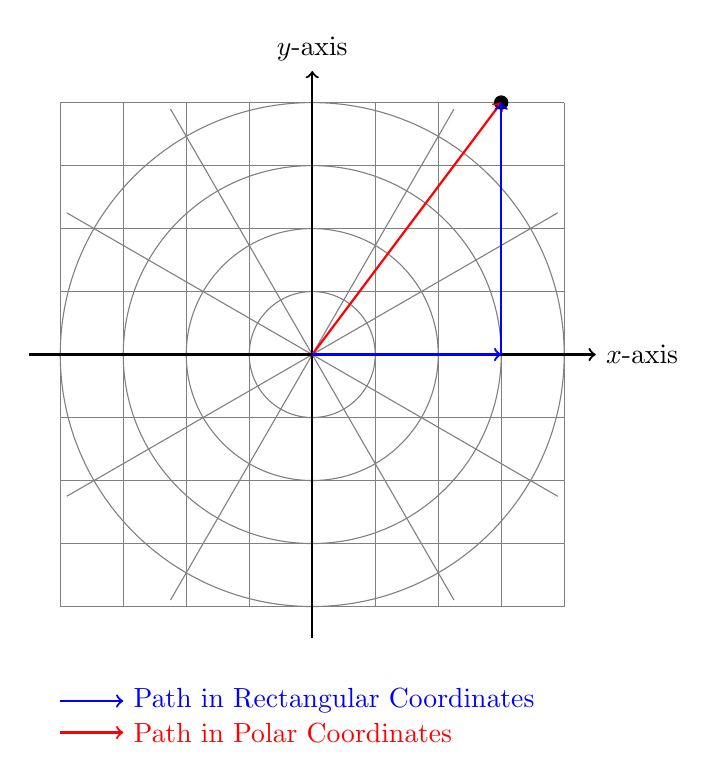
\begin{tikzpicture}[scale=0.8]
        % Draw rectangular grid
        \foreach \x in {-4,-3,-2,-1,1,2,3,4}
            \draw[gray, thin] (\x, -4) -- (\x, 4);
        \foreach \y in {-4,-3,-2,-1,1,2,3,4}
            \draw[gray, thin] (-4, \y) -- (4, \y);

        % Draw polar circles
        \foreach \r in {1,2,3,4}
            \draw[gray, thin] (0,0) circle (\r);

        % Draw polar rays
        \foreach \a in {0,30,60,90,120,150,180,210,240,270,300,330}
            \draw[gray, thin] (0,0) -- (\a:4.5);

        % Label axes
        \draw[thick,->] (-4.5, 0) -- (4.5, 0) node[right] {$x$-axis};
        \draw[thick,->] (0, -4.5) -- (0, 4.5) node[above] {$y$-axis};

        % Plot the point in rectangular coordinates
        \filldraw[black] (3, 4) circle (3pt);

        % Plot the point in polar coordinates (5 units at 53.13 degrees)
        \draw[->, red, thick] (0,0) -- (53.13:5);

        % Blue arrows to show steps reaching (3, 4) along x- and y-axes
        \draw[->, blue, thick] (0, 0) -- (3, 0); % Arrow along x-axis
        \draw[->, blue, thick] (3, 0) -- (3, 4); % Arrow along y-axis

        % Add centered legend at the bottom
        \begin{scope}[shift={(-4, -5.5)}] % Center legend by adjusting x-position in shift
            \draw[thick, blue, ->] (0, 0) -- (1, 0) node[anchor=west] {Path in Rectangular Coordinates};
            \draw[thick, red, ->] (0, -0.5) -- (1, -0.5) node[anchor=west] {Path in Polar Coordinates};
        \end{scope}

    \end{tikzpicture}
    \caption{\textit{Plot showing both Rectangular and Polar representations of the point \( (3, 4) \) with a legend for coordinate paths.}}
    \label{fig:polar_rectangular_plot}
\end{figure}


\subsection*{Cylindrical Coordinates} \index{Cylindrical Coordinates}

The cylindrical coordinate system is an extension of polar coordinates, adding a vertical \( z \)-dimension to describe points in three-dimensional space. It is particularly useful for representing objects with circular symmetry around an axis, such as cylinders, tubes, and circular regions extending along a vertical axis. In cylindrical coordinates, each point is represented by \( (r, \theta, z) \), where:
\begin{itemize}
    \item \( r \): The radial distance from the \( z \)-axis, which is the distance from the point to the \( z \)-axis in the \( xy \)-plane.
    \item \( \theta \): The angle measured from the positive \( x \)-axis within the \( xy \)-plane, in radians, describing the angular position around the \( z \)-axis.
    \item \( z \): The vertical distance from the \( xy \)-plane, equivalent to the \( z \)-coordinate in rectangular coordinates, indicating height or depth.
\end{itemize}

\noindent In essence, cylindrical coordinates generalize polar coordinates by incorporating an additional \( z \)-coordinate, allowing us to describe points in three-dimensional space while maintaining the circular symmetry of polar coordinates around a central axis. If we set \( z = 0 \), cylindrical coordinates reduce to polar coordinates in the \( xy \)-plane, where a point is solely described by its distance \( r \) from the origin and the angle \( \theta \). 

\begin{figure}[H]
    \centering
% Set up the main coordinates for a 3D perspective
\tdplotsetmaincoords{65}{140}

\begin{tikzpicture}[scale=5, tdplot_main_coords]

% Define the radius and z-coordinate
\pgfmathsetmacro{\r}{0.8} % radius
\pgfmathsetmacro{\z}{0.7} % z-coordinate

% Use placeholders for x and y using angle theta
\draw[->, thick] (0,0,0) -- (1.2,0,0) node[anchor=west] {$x$-axis};
\draw[->, thick] (0,0,0) -- (0,1.2,0) node[anchor=west] {$y$-axis};
\draw[->, thick] (0,0,0) -- (0,0,1.2) node[anchor=south] {$z$-axis};

% Draw the vector in cylindrical coordinates
\draw[->, blue!70!black, ultra thick] (0,0,0) -- ({\r*cos(30)},{\r*sin(30)},\z) node[anchor=south] {$(r, \theta, z)$};

% Project to xy-plane
\draw[dashed, blue!50] ({\r*cos(30)},{\r*sin(30)},\z) -- ({\r*cos(30)},{\r*sin(30)},0);
\draw[dashed, blue!50] ({\r*cos(30)},{\r*sin(30)},0) -- (0, 0, 0);

% Draw the circle in the xy-plane to represent radius
\draw[thick, dashed, gray] (0,0,0) circle (\r);

% Draw an arc to indicate the angle theta
\draw[thick, ->, red!70] (0.6,0) arc[start angle=0, end angle=30, radius=0.6];
\node[anchor=west] at (0.35,0.05) {$\theta$};

% Projection points and labels
\filldraw[blue!50] ({\r*cos(30)},{\r*sin(30)},0) circle (0.5pt) node[anchor=north east] {$(r, \theta, 0)$};
\filldraw[blue!50] ({\r*cos(30)},{\r*sin(30)},\z) circle (0.5pt);

% Radius label
\draw[thick, dashed, green!70!black] (0,0,0) -- ({\r*cos(30)},{\r*sin(30)},0);
\node[anchor=north east] at ({\r*cos(15)/2},{\r*sin(15)/2},0) {$r$};

\end{tikzpicture}

    \caption{\textit{A point in three-dimensional space represented in cylindrical coordinates \( (r, \theta, z) \). The radius \( r \) is the distance from the \( z \)-axis, \( \theta \) is the angle measured from the positive \( x \)-axis, and \( z \) is the vertical coordinate.}}
    \label{fig:cylindrical_point_symbolic}
\end{figure}



\noindent Cylindrical coordinates are widely used in fields like physics and engineering where problems often exhibit cylindrical or rotational symmetry. For instance, in analyzing magnetic fields around a wire, fluid flow in pipes, or any phenomenon with a circular base extending along a vertical dimension, cylindrical coordinates provide a natural and efficient way to describe the system.

\subsubsection*{Converting Between Cylindrical and Rectangular Coordinates:}
To switch between cylindrical and rectangular coordinates, we use trigonometric relationships similar to those in polar coordinates, with the \( z \)-coordinate remaining consistent between both systems.

\begin{itemize}
    \item To convert from cylindrical \( (r, \theta, z) \) to rectangular \( (x, y, z) \):
    \[
    x = r \cos \theta, \quad y = r \sin \theta, \quad z = z
    \]
    This transformation projects the point \( (r, \theta) \) in the \( xy \)-plane into \( x \)- and \( y \)-coordinates using trigonometry, while \( z \) remains unchanged.

    \item To convert from rectangular \( (x, y, z) \) to cylindrical \( (r, \theta, z) \):
    \[
    r = \sqrt{x^2 + y^2}, \quad \theta = \tan^{-1} \left( \frac{y}{x} \right), \quad z = z
    \]
    Here, \( r \) is calculated as the distance from the point to the \( z \)-axis (similar to the Pythagorean distance in polar coordinates), and \( \theta \) is the angle around the \( z \)-axis. The \( z \)-coordinate remains the same in both representations.
\end{itemize}

\noindent This conversion framework allows easy switching between cylindrical and rectangular coordinates depending on the symmetry and nature of the problem at hand. In problems with circular symmetry along an axis, cylindrical coordinates simplify analysis and calculation by leveraging the radial and angular structure inherent to the system.


\subsection*{Spherical Coordinates} \index{Spherical Coordinates}

Spherical coordinates are ideal for problems with radial symmetry, such as those involving spheres or radial fields. Each point in spherical coordinates is represented by \( (\rho, \theta, \phi) \):
\begin{itemize}
    \item \( \rho \): The radial distance from the origin (distance from the point to the origin).
    \item \( \theta \): The angle in the \( xy \)-plane from the positive \( x \)-axis, measured counterclockwise.
    \item \( \phi \): The angle between the point and the positive \( z \)-axis (measured from the \( z \)-axis downward).
\end{itemize}

\noindent Spherical coordinates are particularly useful for scenarios where an object moves in a circular arc around a central point and has varying elevation, such as a planet orbiting a star, a camera with full rotation, or a baseball bat’s swing through the air. When a softball player swings a bat to hit a ball, the bat moves in a curved, sweeping motion around the player. The motion of the bat can be best described in spherical coordinates:
\begin{itemize}
    \item Radial Distance (\( \rho \)): The distance of the bat’s tip from the player’s body (the origin) varies, allowing for control over how close or far the bat reaches.
    \item Horizontal Angle (\( \theta \)): The angle \( \theta \) in the \( xy \)-plane represents the circular path of the bat around the player as they swing.
    \item Vertical Angle (\( \phi \)): The vertical angle \( \phi \) describes how high or low the bat is swung, which varies depending on whether the player adjusts to hit a high or low pitch.
\end{itemize}

\begin{figure}[H]
    \centering
\tdplotsetmaincoords{60}{110}
%
\pgfmathsetmacro{\rvec}{.8}
\pgfmathsetmacro{\thetavec}{30}
\pgfmathsetmacro{\phivec}{60}
%
\begin{tikzpicture}[scale=5,tdplot_main_coords]
    \coordinate (O) at (0,0,0);
    \draw[thick,->] (0,0,0) -- (1,0,0) node[anchor=north east]{$x$};
    \draw[thick,->] (0,0,0) -- (0,1,0) node[anchor=north west]{$y$};
\draw[thick,->] (0,0,0) -- (0,0,1) node[anchor=south]{$z$};
    \tdplotsetcoord{P}{\rvec}{\thetavec}{\phivec}
    \draw[-stealth,color=red] (O) -- (P) node[above right] {$\rho$};
    \draw[dashed, color=red] (O) -- (Pxy);
    \draw[dashed, color=red] (P) -- (Pxy);
    \tdplotdrawarc{(O)}{0.2}{0}{\phivec}{anchor=north}{$\phi$}
    \tdplotsetthetaplanecoords{\phivec}
    \tdplotdrawarc[tdplot_rotated_coords]{(0,0,0)}{0.5}{0}%
        {\thetavec}{anchor=south west}{$\theta$}


\end{tikzpicture}
\caption{\textit{A representation of the spherical coordinate system.}}
\end{figure}


\noindent Unlike cylindrical coordinates, which would only capture the horizontal rotation around a central vertical axis (the player’s body), spherical coordinates provide a complete representation of the bat’s path, including its height and depth relative to the player’s position. Thus, spherical coordinates offer a more accurate and flexible framework for capturing the full 3D motion of a softball swing.

\begin{figure}[H]
    \centering
    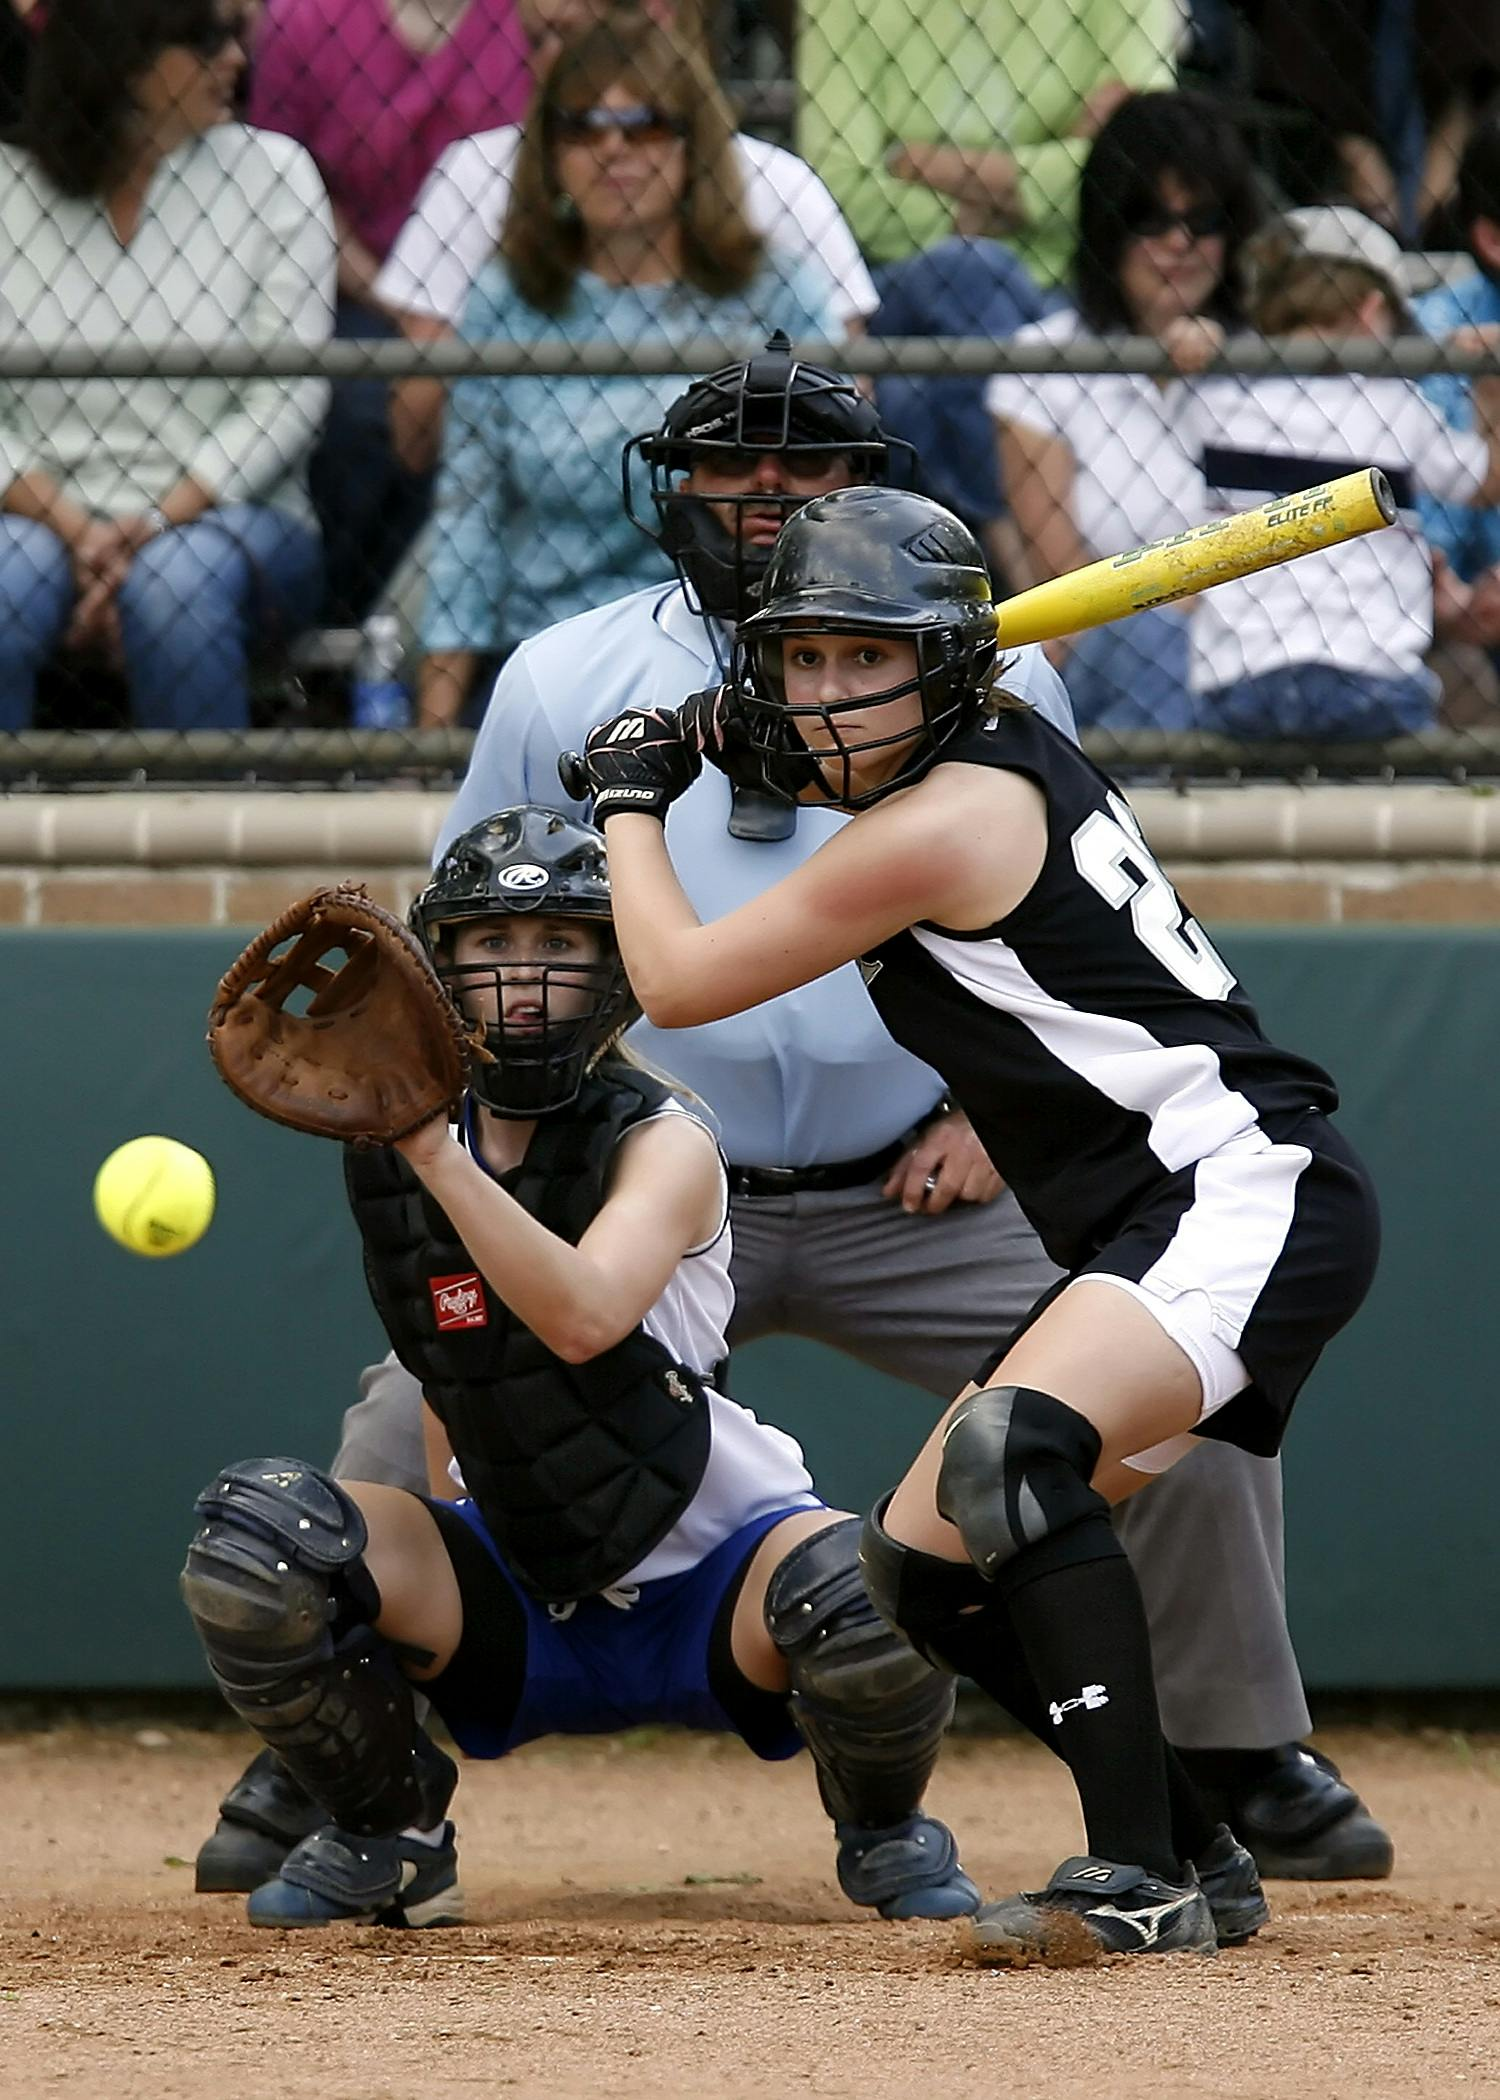
\includegraphics[width=0.3\textwidth]{chapters/chp1_pics/softball.jpg}
    \caption{\textit{A softball swing is best represented in spherical coordinates, capturing the radial distance, horizontal angle, and vertical angle of the bat's position relative to the player.}}
    \label{fig:softball_swing}
\end{figure}

\subsubsection{Converting Between Spherical and Rectangular Coordinates:}
\begin{itemize}
    \item To convert from spherical \( (\rho, \theta, \phi) \) to rectangular \( (x, y, z) \):
    \[
    x = \rho \sin \phi \cos \theta, \quad y = \rho \sin \phi \sin \theta, \quad z = \rho \cos \phi
    \]
    \item To convert from rectangular \( (x, y, z) \) to spherical \( (\rho, \theta, \phi) \):
    \[
    \rho = \sqrt{x^2 + y^2 + z^2}, \quad \theta = \tan^{-1} \left( \frac{y}{x} \right), \quad \phi = \cos^{-1} \left( \frac{z}{\rho} \right)
    \]
\end{itemize}


\exampleline
\begin{example}
A bird is flying along a circular path around a radio tower, while also increasing its altitude. At a certain moment, the bird’s position relative to the tower is given by the cylindrical coordinates \( (r, \theta, z) = (100, \frac{\pi}{4}, 50) \), where \( r \) is in meters and \( z \) represents height. Convert this position into rectangular coordinates to determine the bird’s \( (x, y, z) \) coordinates in the 3D plane.

\begin{solution}
To convert from cylindrical coordinates \( (r, \theta, z) \) to rectangular coordinates \( (x, y, z) \), we use the following conversion formulas:
\[
x = r \cos \theta, \quad y = r \sin \theta, \quad z = z
\]

Given:
\[
r = 100, \quad \theta = \frac{\pi}{4}, \quad z = 50
\]

\begin{enumerate}
    \item Calculate \( x \):
    \[
    x = 100 \cos \frac{\pi}{4} = 100 \cdot \frac{\sqrt{2}}{2} = 50 \sqrt{2}
    \]

    \item Calculate \( y \):
    \[
    y = 100 \sin \frac{\pi}{4} = 100 \cdot \frac{\sqrt{2}}{2} = 50 \sqrt{2}
    \]

    \item The \( z \)-coordinate remains the same:
    \[
    z = 50
    \]

    \item Therefore, the rectangular coordinates of the bird’s position are:
    \[
    (x, y, z) = \left( 50 \sqrt{2}, 50 \sqrt{2}, 50 \right)
    \]
\end{enumerate}

\end{solution}
\end{example}
\exampleline
\begin{example}
In an automated car assembly plant, a spherical robotic arm is used to position car parts in 3D space. The arm operates by extending its length, rotating horizontally, and pivoting vertically. At a certain moment, the robotic arm performs the following actions:

\begin{itemize}
    \item Extends to a length of 2 meters.
    \item Rotates \( 60^\circ \) counterclockwise from the positive \( x \)-axis.
    \item Raises the arm \( 45^\circ \) above the horizontal plane.
\end{itemize}

\noindent Identify which spherical coordinate (\( \rho \), \( \theta \), or \( \phi \)) corresponds to each action, and write down the spherical coordinates of the arm's end effector after this movement.

\begin{solution}
In spherical coordinates:
\begin{itemize}
    \item \( \rho \) represents the distance from the origin to the point (length of the arm).
    \item \( \theta \) is the angle measured in the \( xy \)-plane from the positive \( x \)-axis (horizontal rotation).
    \item \( \phi \) is the angle measured from the positive \( z \)-axis down to the point (vertical angle).
\end{itemize}

Given the actions:

\begin{enumerate}
    \item \textbf{Extension to a length of 2 meters}:
        \begin{itemize}
            \item This corresponds to \( \rho = 2 \, \text{m} \).
        \end{itemize}

    \item \textbf{Rotation \( 60^\circ \) counterclockwise from the positive \( x \)-axis}:
        \begin{itemize}
            \item This corresponds to \( \theta = 60^\circ \) or \( \theta = \dfrac{\pi}{3} \, \text{radians} \).
        \end{itemize}

    \item \textbf{Raising the arm \( 45^\circ \) above the horizontal plane}:
        \begin{itemize}
            \item Since \( \phi \) is measured from the positive \( z \)-axis downwards, we need to calculate \( \phi \).
            \item The horizontal plane corresponds to \( \phi = 90^\circ \) (as it is \( 90^\circ \) down from the positive \( z \)-axis).
            \item Raising the arm \( 45^\circ \) above the horizontal plane means the angle from the positive \( z \)-axis is:
            \[
            \phi = 90^\circ - 45^\circ = 45^\circ \quad \text{or} \quad \phi = \dfrac{\pi}{4} \, \text{radians}.
            \]
        \end{itemize}
\end{enumerate}

\end{solution}
\end{example}
\exampleline

\subsection*{Choice of Coordinates}

The choice of coordinate system is essential in simplifying calculations and providing clarity in solving problems. Each coordinate system has advantages depending on the problem's geometry, symmetry, and underlying physical properties. Below is a comparison of when each system is most useful.

\begin{itemize}
    \item \textbf{Rectangular (Cartesian) Coordinates:} 
    In rectangular coordinates, each point is specified by its perpendicular distances from the \( x \)-, \( y \)-, and \( z \)-axes. This system is intuitive and ideal for objects and problems aligned along the three principal axes, such as rectangular prisms, planes, and many engineering structures.
    \item \textbf{Polar Coordinates:}
    Polar coordinates are well-suited for two-dimensional problems involving circular or rotational symmetry around a central point. Problems that naturally involve rotation or radial symmetry—such as the motion of a particle in a circular path or objects positioned relative to a central point—benefit from polar coordinates.

    \item \textbf{Cylindrical Coordinates:} 
    Cylindrical coordinates are an extension of polar coordinates into three dimensions, making them ideal for problems with circular symmetry around a central vertical axis, such as cylindrical objects or fields surrounding a wire. For example, fluid flow in a pipe, magnetic fields around a wire, or the structure of a cylindrical tank are best analyzed using cylindrical coordinates.

    \item \textbf{Spherical Coordinates:} 
    Spherical coordinates extend the idea of radial symmetry into three dimensions and are best suited for objects and fields with a spherical or radial symmetry, such as planets, stars, and electric fields radiating from a point charge.
\end{itemize}




\newpage


\lecture{Vectors} \index{Vectors}

\noindent In progressing from two-dimensional space to three-dimensional space, vectors become an essential concept for describing both position and direction. Vectors allow us to represent not only points but also the direction and magnitude of movement or force in space, forming the basis for advanced topics in calculus.

\subsection*{Definition of Vectors}

\noindent As we move from two-dimensional space into three dimensions, vectors become crucial for describing both position and direction. Vectors aren’t just about marking a location—they let us describe how something moves or acts, combining both its size (magnitude) and direction. This combination of information forms the basis of advanced ideas in calculus, physics, and engineering. For instance, knowing the strength of a wind gust without knowing the direction isn’t very helpful. But by representing it as a vector, we gain both its intensity and the path it follows. \\ \\ We represent a vector in three-dimensional space with an ordered triple \( \mathbf{v} =\langle v_x, v_y, v_z \rangle \), where:
\begin{itemize}
    \item \( v_x \): Shows the vector’s reach along the \( x \)-axis.
    \item \( v_y \): Shows its reach along the \( y \)-axis.
    \item \( v_z \): Shows its reach along the \( z \)-axis.
\end{itemize}

\noindent Each component captures the vector’s effect along one axis, allowing it to describe anything with direction and magnitude. In addition to using \( \mathbf{v}\), we may also write \( \vec{v} \). This is typically what students write in their notebooks when indicating a vector. For listing components of a vector we may write either \( (v_x, v_y, v_z) \) or \( \langle v_x, v_y, v_z \rangle \). To eliminate ambiguity from describing points, we will use the latter notation. \\ \\ To make vectors more tangible, imagine them as arrows in space. Each arrow’s direction and length tell us the direction and strength of an action or movement—like the current in a river. At each point along the river, an arrow (or vector) can show how fast and in which direction the water flows. Vectors make it possible to describe these continuous, directed motions, making them ideal for representing physical forces or speeds in space. \\ \\ Vectors also have special properties that make them versatile tools. For example, they can be moved around in space without changing their meaning, a property called \textit{translational invariance}. This means a vector maintains its effect regardless of its starting point, allowing us to describe forces or velocities that act consistently no matter where they occur. They can also be ``stacked” or added together, which is essential in physics. For example, if two people push a box from different directions, the net effect on the box’s movement can be represented by the sum of their vectors. Vectors can also be scaled up or down, describing changes in strength or intensity. For example, if a car speeds up, its velocity vector is scaled up to reflect its increased speed while keeping the same direction. This operation, called \textit{scalar multiplication}, lets us adjust vectors without altering their paths.

\begin{figure}[H]
    \centering
% Set up the main coordinates for a 3D perspective, shifted slightly left
\tdplotsetmaincoords{65}{140}

\begin{tikzpicture}[scale=5, tdplot_main_coords]

% Define points for a vector in 3D
\pgfmathsetmacro{\vx}{0.6}
\pgfmathsetmacro{\vy}{0.5}
\pgfmathsetmacro{\vz}{0.7}

% Draw axes
\draw[->, thick] (0,0,0) -- (1.2,0,0) node[anchor=west] {$x$-axis};
\draw[->, thick] (0,0,0) -- (0,1.2,0) node[anchor=west] {$y$-axis};
\draw[->, thick] (0,0,0) -- (0,0,1.2) node[anchor=south] {$z$-axis};

% Draw the main vector from the origin to (vx, vy, vz)
\draw[->, blue!70!black, ultra thick] (0,0,0) -- (\vx,\vy,\vz) node[anchor=south] {$(x, y, z)$};

% Project dashed lines to each coordinate plane
\draw[dashed, blue!50] (\vx, \vy, \vz) -- (\vx, \vy, 0);  % xy-plane
\draw[dashed, blue!50] (\vx, \vy, \vz) -- (\vx, 0, \vz);  % xz-plane
\draw[dashed, blue!50] (\vx, \vy, \vz) -- (0, \vy, \vz);  % yz-plane

% Projection points
\filldraw[blue!50] (\vx, \vy, 0) circle (0.5pt);
\filldraw[blue!50] (\vx, 0, \vz) circle (0.5pt);
\filldraw[blue!50] (0, \vy, \vz) circle (0.5pt);

\end{tikzpicture}

    \caption{\textit{A vector in three-dimensional space represented by components along \( x \), \( y \), and \( z \) axes.}}
    \label{fig:3d_vector}
\end{figure}


\subsection*{Vector Magnitude and Direction}

\noindent The \textit{magnitude} or \textit{length} of a vector \( \mathbf{v} = \langle v_x, v_y, v_z \rangle \) is denoted by \( |\mathbf{v}| \) (and in some advanced texts as \( \| \mathbf{v} \| \)) and is calculated by using the Pythagorean theorem extended to three dimensions. This is because each component of the vector \( v_x \), \( v_y \), and \( v_z \) represents the vector’s ``reach” along the \( x \)-, \( y \)-, and \( z \)-axes. The magnitude formula is directly related to the distance formula covered previously:
\[
|\mathbf{v}| = \sqrt{v_x^2 + v_y^2 + v_z^2}.
\]

\noindent For example, if \( \mathbf{v} = (3, -4, 12) \), then:
\[
|\mathbf{v}| = \sqrt{3^2 + (-4)^2 + 12^2} = \sqrt{9 + 16 + 144} = \sqrt{169} = 13.
\]

\noindent The magnitude provides a sense of ``how much” or ``how far” the vector reaches in space, without giving any indication of direction. With magnitude, we gain a crucial part of the vector’s identity, as it represents the scale or intensity of whatever the vector is describing—such as the speed of a moving object or the strength of a force.

\subsubsection*{Unit Vectors and Direction Cosines}

\noindent A \textit{unit vector} is a vector that has been scaled to have a magnitude of exactly 1 while keeping its direction unchanged. Unit vectors serve as pure directional indicators, providing only the direction without any size or scale. They are especially useful for defining the principal directions along each axis in three-dimensional space. In three-dimensional space, we define the standard unit vectors along the \( x \)-, \( y \)-, and \( z \)-axes as:
\[
\mathbf{i} = \langle 1, 0, 0 \rangle, \quad \mathbf{j} = \langle 0, 1, 0 \rangle, \quad \mathbf{k} = \langle0, 0, 1 \rangle.
\]
\noindent These vectors—\( \mathbf{i} \), \( \mathbf{j} \), and \( \mathbf{k} \)—represent the directions along each principal axis with a magnitude of 1, making them ideal for constructing and breaking down other vectors. In other texts you may also see them written as \( \mathbf{\hat{i}} \), \( \mathbf{\hat{j}} \), and \( \mathbf{\hat{k}} \). Typically important unit vectors are also written this way with a hat. Any vector \( \mathbf{v} = \langle v_x, v_y, v_z \rangle \) can be written in terms of \( \mathbf{i} \), \( \mathbf{j} \), and \( \mathbf{k} \) as:
\[
\mathbf{v} = v_x \mathbf{i} + v_y \mathbf{j} + v_z \mathbf{k}.
\]
\noindent Expressing vectors in this form allows us to separate and analyze their individual components along each axis, which simplifies many operations in vector algebra and physics. To create a unit vector \( \mathbf{u} \) that points in the same direction as a given vector \( \mathbf{v} \), we divide \( \mathbf{v} \) by its magnitude \( |\mathbf{v}| \). For a vector \( \mathbf{v} = (v_x, v_y, v_z) \), the unit vector \( \mathbf{u} \) in the direction of \( \mathbf{v} \) is:
\[
\mathbf{u} = \frac{\mathbf{v}}{|\mathbf{v}|} = \left\langle \frac{v_x}{|\mathbf{v}|}, \frac{v_y}{|\mathbf{v}|}, \frac{v_z}{|\mathbf{v}|} \right\rangle.
\]


\noindent This process of scaling a vector to make it a unit vector is called \textit{normalization}. Normalization allows us to create a standardized version of any vector that preserves its direction while adjusting its magnitude to exactly 1. We will see normal vectors all over this entire study of multi-variable Calculus--more to be addressed about this soon. \\ \\ The concept of unit vectors is valuable in many applications because they give us a standardized way to indicate direction independently of magnitude. For instance, if we only care about the direction an object is moving (such as ``due north”) and not its speed, we can use a unit vector to represent that direction without indicating scale. \\ \\ \textbf{Direction cosines} \index{Direction Cosines} are another way to describe a vector’s direction, using trigonometric relationships to find the angles the vector makes with each coordinate axis. For a vector \( \mathbf{v} = \langle v_x, v_y, v_z \rangle \), direction cosines are the cosines of the angles \( \alpha \), \( \beta \), and \( \gamma \) that \( \mathbf{v} \) makes with the \( x \)-, \( y \)-, and \( z \)-axes, respectively. They are calculated by dividing each component of the vector by its magnitude, which corresponds to taking the cosine of each directional angle:
\[
\cos \alpha = \frac{v_x}{|\mathbf{v}|}, \quad \cos \beta = \frac{v_y}{|\mathbf{v}|}, \quad \cos \gamma = \frac{v_z}{|\mathbf{v}|}.
\]

\noindent The use of cosines here is rooted in trigonometry: when a vector is projected onto an axis, the cosine of the angle gives the ratio between the length of the projection (the component) and the length of the vector itself. This relationship provides a way to understand how the vector is oriented relative to each axis, which is essential in fields like physics and engineering, where precise direction often matters as much as magnitude.


\begin{figure}[H]
    \centering
    \begin{tikzpicture}
        % Draw axes
        \draw[thick,->] (-1,0) -- (5,0) node[right] {$x$-axis};
        \draw[thick,->] (0,-1) -- (0,4) node[above] {$y$-axis};
        
        % Draw vector v
        \draw[thick,->,blue] (0,0) -- (4,3) node[anchor=south west] {$\mathbf{v}$};

        % Project vector v onto x-axis
        \draw[dashed] (4,3) -- (4,0) node[anchor=north] {$v_x$};
        \draw[dashed] (4,3) -- (0,3) node[anchor=east] {$v_y$};

        % Label angle theta
        \draw[thick,->] (1,0) arc[start angle=0,end angle=36.87,radius=1] node[midway, right] {$\theta$};

        % Show magnitude of vector v with customizable position
        \node (magnitude) at (2.2,2) {$|\mathbf{v}|$}; % Moveable label

        % Optional: Add a label you can position manually
        % Uncomment and adjust coordinates to place $|\mathbf{v}|$ in a new location
        % \node at (custom_x, custom_y) {$|\mathbf{v}|$};
    \end{tikzpicture}
    \caption{\textit{A 2D vector \( \mathbf{v} \) showing the angle \( \theta \) with the \( x \)-axis. The direction cosine, \( \cos \theta \), is the ratio \( \frac{v_x}{|\mathbf{v}|} \), which describes the vector’s orientation relative to the \( x \)-axis.}}
    \label{fig:direction_cosines}
\end{figure}


\subsubsection*{Normal Vectors}

\noindent \noindent While direction cosines help us understand how a vector is oriented relative to our coordinate axes, we often need to describe vectors that are perpendicular to other vectors or surfaces. This leads us to the concept of normal vectors. \\

\noindent A \textit{normal vector} (or simply a \textit{normal}) is a vector $\mathbf{n}$ that is perpendicular to something else, like a line or a surface. Normal vectors are especially useful because many problems in physics and geometry involve perpendicular directions. For example, when light hits a mirror, we need to know the direction perpendicular to the mirror's surface to determine how the light will reflect. \\

\noindent For a line in two dimensions, if we know a vector along the line, we can find a normal vector by simply swapping its $x$ and $y$ components and making one of them negative. For example, if a vector along a line is \( \mathbf{v} = \langle 3, 4 \rangle \), then \( \mathbf{n} = \langle -4, 3 \rangle \) is a normal vector to that line. We can verify this is true because perpendicular vectors have components that, when multiplied and summed, equal zero: \( 3(-4) + 4(3) = -12 + 12 = 0 \). \\

\noindent  In polar coordinates, we can find normal vectors in a similar way. For instance, at any point on the circle where \( r = 1 \), a vector pointing outward from the circle (normal to the circle) has components \( \langle \cos\theta, \sin\theta \rangle \). You can visualize this by imagining the normal vector as pointing straight out from the circle at each point, like spokes on a wheel. \\




\noindent Just like any other vector, we can turn a normal vector into a unit normal vector by dividing by its length. Sometimes we denote this like our unit vectors $\mathbf{\hat{n}}$. For instance, in our first example:
\[
\mathbf{\hat{n}} = \frac{\langle -4, 3 \rangle}{\sqrt{(-4)^2 + 3^2}} = \frac{\langle -4, 3 \rangle}{5} = \left\langle -\frac{4}{5}, \frac{3}{5} \right\rangle.
\]

\noindent Unit normal vectors as we have seen are useful because they give us a standard way to describe perpendicular directions, regardless of the size of the original vectors we started with. We'll see many applications of normal vectors as we continue our study of vectors and their uses in geometry and physics.

\begin{figure}[H]
    \centering
    \begin{minipage}{0.48\textwidth}
        \centering
        \begin{tikzpicture}[scale=1]
            % Cartesian axes
            \draw[thick,->] (-2,0) -- (4,0) node[right] {$x$};
            \draw[thick,->] (0,-2) -- (0,4) node[above] {$y$};
            
            % Original vector
            \draw[thick,->,blue] (0,0) -- (3,2) node[anchor=west] {$\mathbf{v}$};
            
            % Normal vector (perpendicular)
            \draw[thick,->,red] (0,0) -- (-2,3) node[anchor=south] {$\mathbf{n}$};
           
            
        \end{tikzpicture}
        \caption*{(a) Normal vector in Cartesian coordinates}
    \end{minipage}
    \begin{minipage}{0.48\textwidth}
        \centering
        \begin{tikzpicture}[scale=1]
            % Draw the unit circle
            \draw[thick] (0,0) circle (2);
            
            % Axes
            \draw[thick,->] (-2.5,0) -- (2.5,0) node[right] {$x$};
            \draw[thick,->] (0,-2.5) -- (0,2.5) node[above] {$y$};
            
            % Point on circle at theta = pi/4
            \coordinate (P) at (45:2);
            
            % Radial vector (to point on circle)
            \draw[thick,->,blue] (0,0) -- (P) node[anchor=south west] {$\mathbf{r}$};
            
            % Normal vector (tangent to circle)
            \draw[thick,->,red] (P) -- ($(P)+(135:1.5)$) node[anchor=south] {$\mathbf{n}$};
            
            % Angle label
            \draw[thick] (0.5,0) arc (0:45:0.5) node[midway,above right] {$\theta$};
            
        \end{tikzpicture}
        \caption*{(b) Normal vector on a circle (polar)}
    \end{minipage}
    \caption{\textit{Normal vectors shown in different coordinate systems. In (a), the normal vector $\mathbf{n}$ is perpendicular to vector $\mathbf{v}$. In (b), the normal vector $\mathbf{n}$ is perpendicular to the radial vector $\mathbf{r}$ at a point on the circle.}}
    \label{fig:normal_vectors}
\end{figure}

\exampleline
\begin{example}
A heavy box is being pushed along a factory floor with a force vector \( \mathbf{F} = \langle 9, 12, 15 \rangle \) (measured in newtons) representing the components of the force applied along the \( x \)-, \( y \)-, and \( z \)-axes. Find the magnitude of \( \mathbf{F} \), determine the unit vector in the direction of \( \mathbf{F} \), calculate the direction cosines of \( \mathbf{F} \) with respect to each axis, and find a normal vector to \( \mathbf{F} \) that lies in the $xy$-plane.

\begin{solution}
To find the unit vector and direction cosines, we first need the magnitude of \( \mathbf{F} \).

\begin{enumerate}
    \item Calculate the magnitude \( |\mathbf{F}| \) using the formula:
    \[
    |\mathbf{F}| = \sqrt{F_x^2 + F_y^2 + F_z^2}
    \]
    Substitute \( F_x = 9 \), \( F_y = 12 \), and \( F_z = 15 \):
    \[
    |\mathbf{F}| = \sqrt{9^2 + 12^2 + 15^2} = \sqrt{81 + 144 + 225} = \sqrt{450} = 15\sqrt{2}
    \]

    \item Now, calculate the unit vector \( \mathbf{u} \) in the direction of \( \mathbf{F} \):
    \[
    \mathbf{u} = \frac{\mathbf{F}}{|\mathbf{F}|} = \left\langle \frac{9}{15\sqrt{2}}, \frac{12}{15\sqrt{2}}, \frac{15}{15\sqrt{2}} \right\rangle
    \]
    Simplify each component:
    \[
    \mathbf{u} = \left\langle \frac{3}{5\sqrt{2}}, \frac{4}{5\sqrt{2}}, \frac{1}{\sqrt{2}} \right\rangle
    \]

    \item Next, we calculate the direction cosines, which are the cosines of the angles that \( \mathbf{F} \) makes with each coordinate axis. These are given by:
    \[
    \cos \alpha = \frac{F_x}{|\mathbf{F}|}, \quad \cos \beta = \frac{F_y}{|\mathbf{F}|}, \quad \cos \gamma = \frac{F_z}{|\mathbf{F}|}
    \]
    
    Substitute the values of \( F_x \), \( F_y \), \( F_z \), and \( |\mathbf{F}| = 15\sqrt{2} \):
    \begin{align*}
        \cos \alpha &= \frac{9}{15\sqrt{2}} = \frac{3}{5\sqrt{2}} \\
        \cos \beta &= \frac{12}{15\sqrt{2}} = \frac{4}{5\sqrt{2}} \\
        \cos \gamma &= \frac{15}{15\sqrt{2}} = \frac{1}{\sqrt{2}}
    \end{align*}

\item Finally, let's find a normal vector to \( \mathbf{F} \) that lies in the $xy$-plane. We can do this by:
\begin{itemize}
    \item First, considering only the $x$ and $y$ components of \( \mathbf{F} \): \( \langle 9, 12 \rangle \)
    \item To find a normal vector in 2D, we can swap these components and make one negative: \( \langle -12, 9 \rangle \)
    \item Since we want this normal vector in 3D space lying in the xy-plane, we add a $z$-component of $0$
\end{itemize}
Therefore, one possible normal vector is \( \mathbf{n} = \langle -12, 9, 0 \rangle \).

We can verify this is indeed perpendicular to \( \mathbf{F} \) by checking if their dot product is zero:
\[
\mathbf{F} \cdot \mathbf{n} = 9(-12) + 12(9) + 15(0) = -108 + 108 + 0 = 0
\]

\item Therefore, our complete results are:
\begin{itemize}
\item The magnitude of \( \mathbf{F} \) is \( 15\sqrt{2} \) newtons.
\item The unit vector in the direction of \( \mathbf{F} \) is \( \mathbf{u} = \left\langle \frac{3}{5\sqrt{2}}, \frac{4}{5\sqrt{2}}, \frac{1}{\sqrt{2}} \right\rangle \).
\item The direction cosines are:
\[
\cos \alpha = \frac{3}{5\sqrt{2}}, \quad \cos \beta = \frac{4}{5\sqrt{2}}, \quad \cos \gamma = \frac{1}{\sqrt{2}}
\]
\item A normal vector to \( \mathbf{F} \) in the xy-plane is \( \mathbf{n} = \langle -12, 9, 0 \rangle \).
    \end{itemize}
\end{enumerate}

\end{solution}
\end{example}
\exampleline







\subsection*{Vector Operations} \index{Vector Operations}

Vectors can be added, subtracted, and scaled, enabling a wide range of applications. Understanding vector operations involves grasping both their mathematical properties and the intuitive idea of combining directions and magnitudes.

\subsubsection*{Vector Addition and Subtraction}

\noindent Vector addition is done by adding corresponding components. Given two vectors \( \mathbf{u} = \langle u_x, u_y, u_z \rangle \) and \( \mathbf{v} = \langle v_x, v_y, v_z \rangle \), their sum \( \mathbf{u} + \mathbf{v} \) is calculated by adding each component individually:
\[
\mathbf{u} + \mathbf{v} = \langle u_x + v_x, u_y + v_y, u_z + v_z\rangle.
\]
Similarly, the difference \( \mathbf{u} - \mathbf{v} \) is given by:
\[
\mathbf{u} - \mathbf{v} = \langle u_x - v_x, u_y - v_y, u_z - v_z \rangle.
\]

\noindent The reason we can add vector components directly is that each component describes how far the vector reaches along a particular axis. When we add the components, we’re combining these ``reaches” along each axis into a single, unified reach, effectively determining where we’d end up if we followed each vector sequentially. \\ \\ An intuitive way to think about vector addition is with the \textit{tip-to-tail} method. In this method, we place the tail (starting point) of \( \mathbf{v} \) at the tip (ending point) of \( \mathbf{u} \), without changing either vector’s length or direction. This use of \textit{translational invariance} that we previously talked about means the vectors can be moved around in space without changing their meaning, as their direction and magnitude stay the same. The resulting vector, drawn from the starting point of \( \mathbf{u} \) to the tip of \( \mathbf{v} \), represents the sum \( \mathbf{u} + \mathbf{v} \). This tip-to-tail method visually demonstrates how two directions and magnitudes combine to create a new direction and magnitude.

\begin{figure}[H]
    \centering
    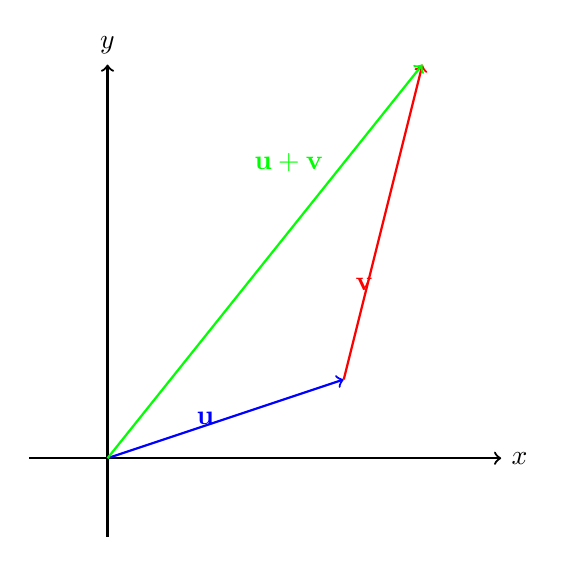
\begin{tikzpicture}
        % Axes
        \draw[thick,->] (-1,0) -- (5,0) node[right] {$x$};
        \draw[thick,->] (0,-1) -- (0,5) node[above] {$y$};

        % Vectors with tip-to-tail alignment
        \draw[thick,->,blue] (0,0) -- (3,1) node[anchor=south west] at (1,0.3) {$\mathbf{u}$};
        \draw[thick,->,red] (3,1) -- (4,5) node[anchor=south east] at (3.5,2) {$\mathbf{v}$}; % Position v at the tip of u
        \draw[thick,->,green] (0,0) -- (4,5) node[anchor=south] at (2.3,3.5) {$\mathbf{u} + \mathbf{v}$}; % Resultant vector
    \end{tikzpicture}
    \caption{\textit{Tip-to-tail method of vector addition: placing \( \mathbf{v} \) at the tip of \( \mathbf{u} \) results in \(\mathbf{u} + \mathbf{v}\).}}
    \label{fig:vector_addition}
\end{figure}

\noindent \textbf{Analogy: Tug of War.} Consider a classic game of tug-of-war: two teams pull on opposite sides of a rope that has a flag tied in the middle. Each team’s force is represented by a vector. If two people on one team each pull with forces represented by vectors \( \mathbf{u} \) and \( \mathbf{v} \), their combined effort is represented by the sum \( \mathbf{u} + \mathbf{v} \), a vector with a magnitude and direction determined by the tip-to-tail addition. If the teams pull at equal effort, the vectors which are the same length, can be combined tip to tail which would go out and then right back to the flag in the middle, meaning the flag won't move. \\ \\ Now, we can extend this idea: is a three-dimensional tug-of-war possible? Imagine a 3D tug-of-war where three teams pull the rope in different directions. Each team’s force is represented by a vector, and the resulting motion of the rope would depend on the sum of all these vectors. In 3D, vector addition still combines each vector’s pull, and the rope would move in the direction of the resulting vector. However, the outcome could be complex, with the rope moving in a new diagonal direction rather than towards one “winning” team. This idea illustrates how vector addition generalizes even when multiple forces act in various directions.\\ \\ We can see where we would place our \( \mathbf{u} \) and \( \mathbf{v} \)  vectors in the below picture:

\begin{figure}[H]
    \centering
    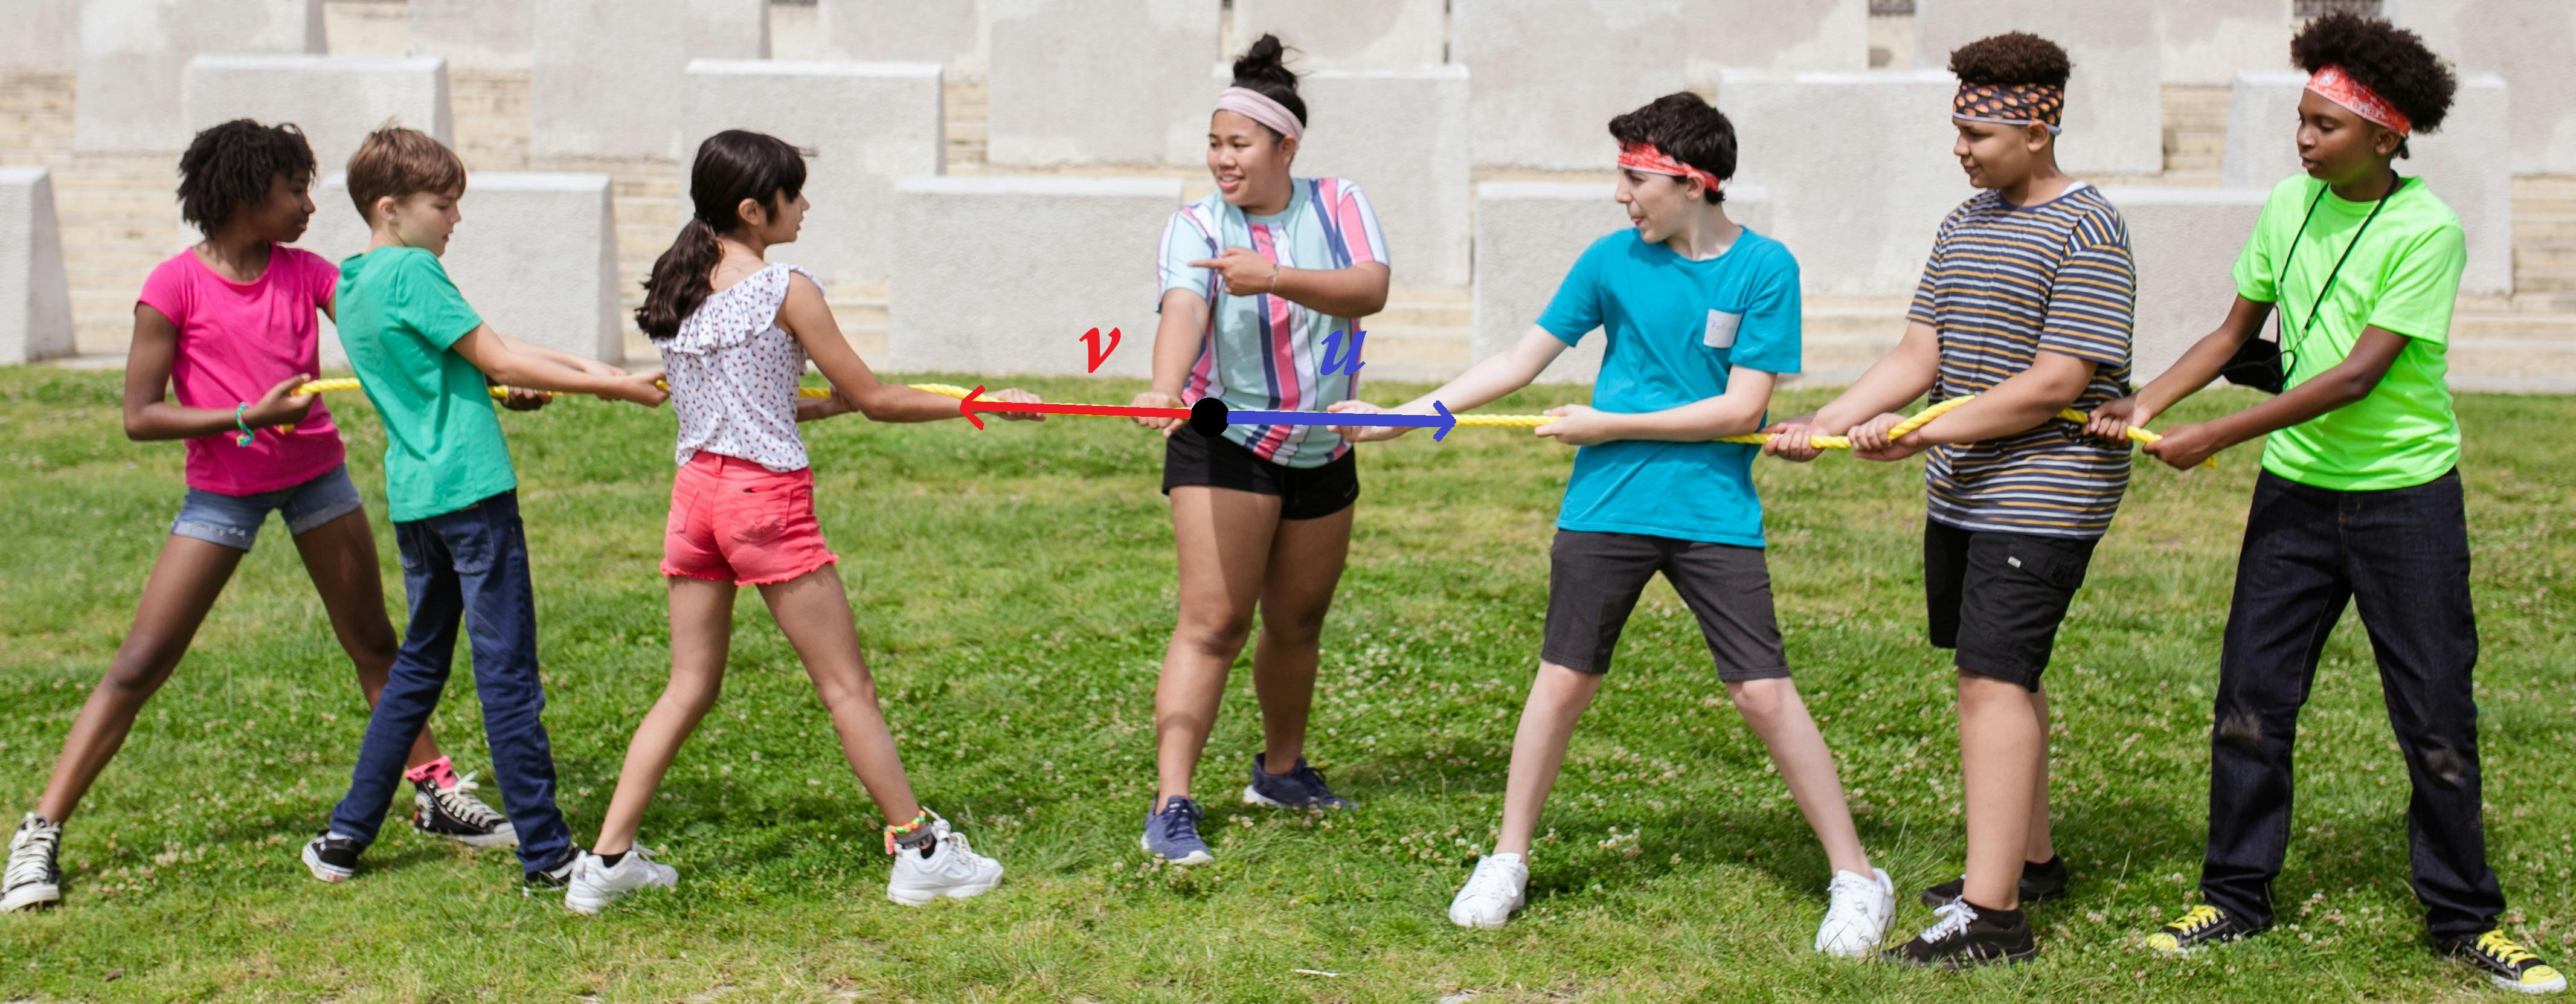
\includegraphics[width=0.7\textwidth]{chapters/chp1_pics/tugofwar_vec.jpg}
    \caption{\textit{Tug-of-war as a visual analogy for vector addition.}}
    \label{fig:tug_of_war}
\end{figure}

\noindent We may also consider by itself, a negative vector \(-\mathbf{v} \) with the same magnitude but an opposite direction. For a vector \( \mathbf{v} \), the negative vector \( -\mathbf{v} \) reverses all components:
\[
-\mathbf{v} = \langle -v_x, -v_y, -v_z \rangle.
\]
\noindent Negative vectors are useful in subtraction, as subtracting a vector is the same as adding its negative: \( \mathbf{u} - \mathbf{v} = \mathbf{u} + (-\mathbf{v}) \).

\subsubsection*{Scalar Multiplication}

\noindent Scalar multiplication scales a vector by a constant factor. If \( c \) is a scalar and \( \mathbf{v} = \langle v_x, v_y, v_z \rangle \), then:
\[
c\mathbf{v} = \langle c v_x, c v_y, c v_z \rangle.
\]

\noindent This means that each component of \( \mathbf{v} \) is multiplied by \( c \), effectively stretching or shrinking the vector by a factor of \( c \). If \( c > 1 \), the vector’s magnitude increases; if \( 0 < c < 1 \), it decreases. \\ \\ For example, doubling the force in a tug-of-war scenario would double each component of the vector representing that force, effectively making the pull twice as strong but in the same direction. Together, vector addition and scalar multiplication allow us to construct complex combinations of vectors and to adjust their magnitudes while maintaining direction, providing a powerful foundation for vector operations in physics and engineering. We may visualize the negative vector and scalar multiplication on the graph below:

\begin{figure}[H]
    \centering
    \begin{tikzpicture}
        % Axes
        \draw[thick,->] (-4,0) -- (5,0) node[right] {$x$};
        \draw[thick,->] (0,-3) -- (0,5) node[above] {$y$};

        % Original vector v with manual label positioning
        \draw[ultra thick,->,blue] (0,0) -- (3,2);
        \node[anchor=north west] at (1.6,1.2) {$\mathbf{v}$};

        % Negative vector -v with manual label positioning
        \draw[ultra thick,->,red] (0,0) -- (-3,-2);
        \node[anchor=north east] at (-1.5,-0.5) {$-\mathbf{v}$};

        % Scaled vector (1/2)v with manual label positioning
        \draw[ultra thick,->,green] (0,0) -- (1.5,1);
        \node[anchor=south west] at (1,0.05) {$\frac{1}{2}\mathbf{v}$};

        % Scaled vector 1.5v with manual label positioning
        \draw[ultra thick,->,purple] (0,0) -- (4.5,3);
        \node[anchor=south east] at (3,2.5) {$1.5\mathbf{v}$};
    \end{tikzpicture}
    \caption{\textit{A vector \( \mathbf{v} \) and its negative counterpart \( -\mathbf{v} \), along with scalar multiples of \( \mathbf{v} \) for various constants.}}
    \label{fig:vector_scalar_multiplication}
\end{figure}

\exampleline
\begin{example}
An engineer is designing a crane to lift materials by applying forces from multiple cables to achieve the required lift and stability. At a particular moment, two cables exert forces represented by the vectors \( \mathbf{F_1} = \langle 120, 0, 80 \rangle \) and \( \mathbf{F_2} = \langle -50, 75, 60 \rangle \), measured in newtons. To achieve a stable lift, determine the combined force applied by both cables, calculate the unit vector in the direction of the combined force, and find a third vector \( \mathbf{G} \) that would need to be added to triple the resultant force from the two cables. Additionally, if we need to fully stabilize the system, calculate the force vector for a third cable \( \mathbf{F_3} \) that would completely counterbalance the combined force.

\begin{solution}
To solve this problem, we’ll use vector addition, scalar multiplication, unit vector concepts, and explore how to achieve both triple force and full stability.

\begin{enumerate}
    \item Combine the Forces by Vector Addition: The combined force vector \( \mathbf{F} = \mathbf{F_1} + \mathbf{F_2} \) is found by adding the components of \( \mathbf{F_1} \) and \( \mathbf{F_2} \):
    \[
    \mathbf{F} = \langle 120 + (-50), 0 + 75, 80 + 60 \rangle = \langle 70, 75, 140 \rangle
    \]

    \item Calculate the Magnitude of the Combined Force: The magnitude \( |\mathbf{F}| \) of the combined force vector \( \mathbf{F} \) is given by:
    \[
    |\mathbf{F}| = \sqrt{70^2 + 75^2 + 140^2} = \sqrt{4900 + 5625 + 19600} = \sqrt{30125} \approx 173.6 \text{ newtons}
    \]

    \item Find the Unit Vector in the Direction of the Combined Force: The unit vector \( \mathbf{u} \) in the direction of \( \mathbf{F} \) is calculated by dividing each component by \( |\mathbf{F}| \):
    \[
    \mathbf{u} = \frac{\mathbf{F}}{|\mathbf{F}|} = \left\langle \frac{70}{173.6}, \frac{75}{173.6}, \frac{140}{173.6} \right\rangle \approx \langle 0.403, 0.432, 0.806 \rangle
    \]

    \item Determine the Vector \( \mathbf{G} \) to Triple the Combined Force: To triple the resultant force, we need a new vector \( \mathbf{G} \) such that the total force becomes \( 3\mathbf{F} \). This means:
    \[
    \mathbf{G} = 3\mathbf{F} - \mathbf{F} = 2\mathbf{F} = 2 \times \langle 70, 75, 140 \rangle = \langle 140, 150, 280 \rangle
    \]
    Therefore, the vector \( \mathbf{G} \) that would need to be applied to triple the combined force is:
    \[
    \mathbf{G} = \langle 140, 150, 280 \rangle
    \]

    \item Determine the Counterbalancing Force Vector \( \mathbf{F_3} \): To fully stabilize the system, we need a third cable with force vector \( \mathbf{F_3} \) that exactly counterbalances the combined force \( \mathbf{F} \). This means \( \mathbf{F_3} \) must be equal in magnitude but opposite in direction to \( \mathbf{F} \), so:
    \[
    \mathbf{F_3} = -\mathbf{F} = \langle -70, -75, -140 \rangle
    \]
    Applying this force would bring the net force to zero, stabilizing the system entirely.

\end{enumerate}

\noindent Thus, the combined force vector of the two cables is \( \langle 70, 75, 140 \rangle \) newtons, with a unit direction vector \( \langle 0.403, 0.432, 0.806 \rangle \). To triple this force, a third vector \( \mathbf{G} = \langle 140, 150, 280 \rangle \) would be added. Finally, a fourth force vector, cable three, \( \mathbf{F_3} = \langle -70, -75, -140 \rangle \) would stabilize the system by perfectly counterbalancing the combined force.

\end{solution}
\end{example}
\exampleline


\vspace{1.3em}


\noindent We've covered addition and subtraction of vectors, which have intuitive meanings in terms of combining directions and magnitudes. However, multiplication raises an important question: how do we interpret multiplying vectors? Here, the dot and cross products offer two distinct perspectives. The dot product provides a scalar, measuring alignment between vectors, while the cross product results in a new vector, perpendicular to both. Simply multiplying components wouldn’t capture these meaningful outcomes, so dot and cross products arise naturally as solutions to vector multiplication.


\subsection*{Dot Product} \index{Dot Product}

The \textit{dot product} (or scalar product) of two vectors \( \mathbf{u} = \langle u_x, u_y, u_z \rangle \) and \( \mathbf{v} = \langle v_x, v_y, v_z \rangle \) measures how much one vector “projects” onto another. This projection quantifies how much of one vector’s length is aligned in the direction of the other. Mathematically, the dot product is defined as:
\[
\mathbf{u} \cdot \mathbf{v} = u_x v_x + u_y v_y + u_z v_z.
\]
While this formula looks straightforward, it can be re-expressed to reveal a deeper interpretation by relating it to the angle \( \theta \) between \( \mathbf{u} \) and \( \mathbf{v} \):
\[
\mathbf{u} \cdot \mathbf{v} = |\mathbf{u}| |\mathbf{v}| \cos \theta.
\]
This alternate form shows that the dot product depends on the magnitudes of \( \mathbf{u} \) and \( \mathbf{v} \) and their alignment. To understand where \( \cos \theta \) comes into play, recall that we previously introduced direction cosines to describe a vector’s orientation. In the dot product, \( \cos \theta \) arises because the product measures how well-aligned two vectors are. When two vectors point in the same direction, \( \theta = 0 \) (cosine of 0° is 1), and the dot product is simply \( |\mathbf{u}| |\mathbf{v}| \). If the vectors are perpendicular (at 90°, or \( \pi/2 \) radians), \( \cos \theta = 0 \), and the dot product is zero, meaning there’s no overlap in direction.

\begin{figure}[H]
    \centering
    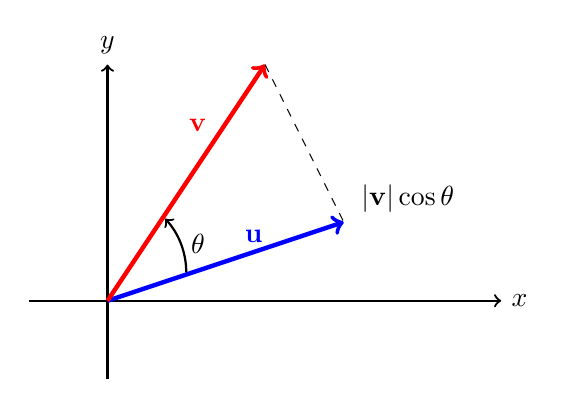
\begin{tikzpicture}
        % Axes
        \draw[thick,->] (-1,0) -- (5,0) node[right] {$x$};
        \draw[thick,->] (0,-1) -- (0,3) node[above] {$y$};
        
        % Vectors u and v
        \draw[ultra thick,->,blue] (0,0) -- (3,1) node[anchor=south west] at (1.6,0.6) {$\mathbf{u}$};
        \draw[ultra thick,->,red] (0,0) -- (2,3) node[anchor=south east] at (1.4,2) {$\mathbf{v}$};
        
        % Projection line from v onto u
        \draw[dashed] (2,3) -- (3,1);
        
        % Angle theta
        \draw[thick,->] (1,.36) arc[start angle=0,end angle=43,radius=1] node[midway, right] {$\theta$};
        
        % Label for |v| cos theta projection
        \node[anchor=north west] at (3.1,1.6) {$|\mathbf{v}| \cos \theta$};
    \end{tikzpicture}
    \caption{\textit{The dot product as the projection of \( \mathbf{v} \) onto \( \mathbf{u} \), scaled by \( \cos \theta \).}}
    \label{fig:dot_product_projection}
\end{figure}

\noindent \textbf{Real-World Example: Work Done by a Force.} A common example of the dot product is the calculation of work done by a force acting over a displacement. If a force \( \mathbf{F} \) is applied to move an object by a displacement \( \mathbf{d} \), then the work done \( W \) is:
\[
W = \mathbf{F} \cdot \mathbf{d} = |\mathbf{F}| |\mathbf{d}| \cos \theta.
\]
In this expression, only the component of the force that aligns with the displacement contributes to work. To make this intuitive, think about closing a door: if you push on the door in a direction perfectly perpendicular to its plane (where \( \theta = 90^\circ \) or \( \pi/2 \)), the force is wasted because \( \cos(90^\circ) = 0 \), and no work is done to close the door. However, when you push directly along the direction of the door’s swing (at \( \theta = 0^\circ \)), the cosine is maximized, allowing the full force to contribute to moving the door. \\ \\ Thus, the dot product is valuable because it captures not just magnitude but the idea of alignment, making it essential in scenarios where only the aligned portion of a force (or vector) is relevant to an outcome.

\exampleline
\begin{example}
Given vectors \( \mathbf{a} = \langle 3, 0, 4 \rangle \) and \( \mathbf{b} = \langle 1, 2, -1 \rangle \), calculate their dot product and interpret the result.

\begin{solution}
The dot product \( \mathbf{a} \cdot \mathbf{b} \) is computed as:
\[
\mathbf{a} \cdot \mathbf{b} = (3)(1) + (0)(2) + (4)(-1).
\]

Calculating each term:
\begin{align*}
    3 \cdot 1 &= 3, \\
    0 \cdot 2 &= 0, \\
    4 \cdot (-1) &= -4.
\end{align*}

Adding these results, we get:
\[
\mathbf{a} \cdot \mathbf{b} = 3 + 0 - 4 = -1.
\]

The dot product \( -1 \) indicates that \( \mathbf{a} \) and \( \mathbf{b} \) are not aligned, as a positive result would imply some degree of alignment in the same direction. The negative value suggests that \( \mathbf{a} \) and \( \mathbf{b} \) point in somewhat opposite directions along their components.

\end{solution}
\end{example}
\exampleline


\subsection*{Cross Product} \index{Cross Product}

The \textit{cross product} (or vector product) of two vectors \( \mathbf{u} = \langle u_x, u_y, u_z \rangle \) and \( \mathbf{v} = \langle v_x, v_y, v_z \rangle \) gives a new vector that is perpendicular, or \textit{normal} to both \( \mathbf{u} \) and \( \mathbf{v} \). The cross product is defined such that the resulting vector points in a direction determined by the \textit{right-hand rule}: if you point your right hand’s index finger along \( \mathbf{u} \) and your middle finger along \( \mathbf{v} \), then your thumb points in the direction of \( \mathbf{u} \times \mathbf{v} \). The magnitude of this vector corresponds to the area of the parallelogram spanned by \( \mathbf{u} \) and \( \mathbf{v} \), given by:
\[
\mathbf{n} = \mathbf{u} \times \mathbf{v} = \langle u_y v_z - u_z v_y, u_z v_x - u_x v_z, u_x v_y - u_y v_x \rangle.
\]

\noindent An alternative way to calculate the cross product is by using the \textit{determinant} of a \( 3 \times 3 \) matrix (maybe you have heard of this in linear algebra before). In this method, we set up a matrix with the unit vectors \( \mathbf{i} \), \( \mathbf{j} \), and \( \mathbf{k} \) in the first row, the components of \( \mathbf{u} \) in the second row, and the components of \( \mathbf{v} \) in the third row:
\[
\mathbf{u} \times \mathbf{v} = \begin{vmatrix} \mathbf{i} & \mathbf{j} & \mathbf{k} \\ u_x & u_y & u_z \\ v_x & v_y & v_z \end{vmatrix}.
\]

To compute this determinant, we expand along the first row:
\[
\mathbf{u} \times \mathbf{v} = \mathbf{i} \begin{vmatrix} u_y & u_z \\ v_y & v_z \end{vmatrix} - \mathbf{j} \begin{vmatrix} u_x & u_z \\ v_x & v_z \end{vmatrix} + \mathbf{k} \begin{vmatrix} u_x & u_y \\ v_x & v_y \end{vmatrix}.
\]

Each \( 2 \times 2 \) determinant is calculated as follows:
\[
\begin{vmatrix} a & b \\ c & d \end{vmatrix} = a d - b c.
\]

Applying this to our cross product:
\[
\mathbf{u} \times \mathbf{v} = \mathbf{i} (u_y v_z - u_z v_y) - \mathbf{j} (u_x v_z - u_z v_x) + \mathbf{k} (u_x v_y - u_y v_x).
\]

Thus, we arrive at the same result as before:
\[
\mathbf{u} \times \mathbf{v} = \langle u_y v_z - u_z v_y, u_z v_x - u_x v_z, u_x v_y - u_y v_x \rangle.
\]

\noindent Using the determinant method provides a structured way to calculate the cross product and reinforces the concept of orientation in three-dimensional space. \\ \\ The magnitude of the cross product is given by:
\[
|\mathbf{u} \times \mathbf{v}| = |\mathbf{u}| |\mathbf{v}| \sin \theta,
\]
where \( \theta \) is the angle between \( \mathbf{u} \) and \( \mathbf{v} \). This value is maximized when \( \mathbf{u} \) and \( \mathbf{v} \) are perpendicular (where \( \sin \theta = 1 \)) and zero when the vectors are parallel, indicating no area spanned.

\noindent The magnitude of the cross product is significant because it represents the area of the parallelogram formed by \( \mathbf{u} \) and \( \mathbf{v} \). \\ \\ Geometrically, this area provides a measure of how ``spread out" the two vectors are relative to each other. If the vectors are aligned (parallel), there’s no area between them, so the magnitude is zero. When the vectors are perpendicular, they span the maximum possible area, with the magnitude equal to \( |\mathbf{u}| |\mathbf{v}| \). This concept is especially useful in physics and engineering, where the cross product’s magnitude can indicate quantities like torque or rotational force, which depend on both the strength and the orientation of the applied forces. We observe a visualization below:

\begin{figure}[H]
    \centering
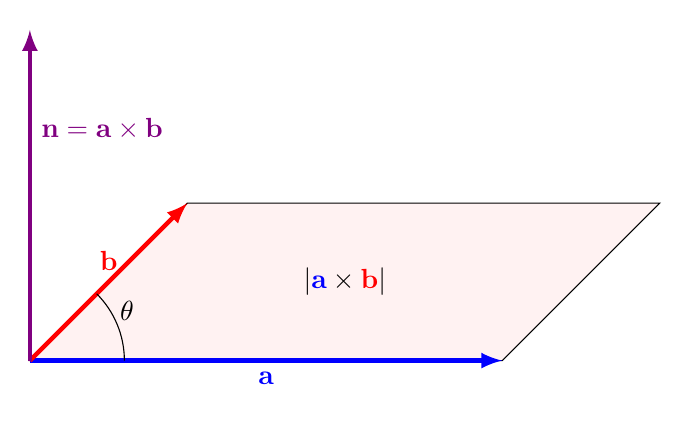
\begin{tikzpicture}[scale=2]
\draw[-,fill=white!95!red](0,0)--(3,0)--(4,1)--(1,1)--cycle;
\node at (2,0.5) {$|\textcolor{blue}{\mathbf{a}}\times \textcolor{red}{\mathbf{b}}|$};
\draw[ultra thick,-latex,blue](0,0)--(3,0)node[midway,below]{$\mathbf{a}$};
\draw[ultra thick,-latex,red](0,0)--(1,1)node[midway,above]{$\mathbf{b}$};
\draw[ultra thick,-latex,blue!50!red](0,0)--(0,2.1)node[pos=0.7,right]{$\mathbf{n} = \mathbf{a}\times \mathbf{b}$};
\draw (0.6,0) arc [start angle=0,end angle=45,radius=0.6]
node[pos=0.7,right]{$\theta$};
\end{tikzpicture}
    \caption{\textit{Visualization of the cross product \( \mathbf{a} \times \mathbf{b} \), showing the area spanned by vectors \( \mathbf{a} \) and \( \mathbf{b} \), as well as the normal vector direction $\mathbf{n}$.}}
    \label{fig:cross_product_area}
\end{figure}

\exampleline
\begin{example}
Compute the following cross products:
\begin{enumerate}
   \item $\langle 1, 5, 7\rangle \times \langle -4, 3, 3.2\rangle$
   \item $\langle xy^2, z^2, x\rangle \times \langle y, x, z\rangle$
\end{enumerate}

\begin{solution}
\begin{enumerate}
   \item Using the determinant method:
   \[
   \begin{vmatrix}
   \mathbf{i} & \mathbf{j} & \mathbf{k} \\
   1 & 5 & 7 \\
   -4 & 3 & 3.2
   \end{vmatrix}
   \]
   \[
   \begin{aligned}
   i &= \begin{vmatrix} 5 & 7 \\ 3 & 3.2 \end{vmatrix} 
       = 5 \cdot 3.2 \;-\; 7 \cdot 3 
       = 16 - 21 
       = -5 \\[1ex]
   j &= -\begin{vmatrix} 1 & 7 \\ -4 & 3.2 \end{vmatrix} 
       = -\bigl(1 \cdot 3.2 - 7 \cdot (-4)\bigr) 
       = -\bigl(3.2 + 28\bigr) 
       = -31.2 \\[1ex]
   k &= \begin{vmatrix} 1 & 5 \\ -4 & 3 \end{vmatrix} 
       = 1 \cdot 3 \;-\; 5 \cdot (-4) 
       = 3 + 20 
       = 23
   \end{aligned}
   \]
   \[
   \langle 1, 5, 7\rangle \times \langle -4, 3, 3.2\rangle 
   = \langle -5, -31.2, 23\rangle
   \]

   \item Using the same method:
   \[
   \begin{vmatrix}
   \mathbf{i} & \mathbf{j} & \mathbf{k} \\
   xy^2 & z^2 & x \\
   y & x & z
   \end{vmatrix}
   \]
   \[
   \begin{aligned}
   i &= \begin{vmatrix} z^2 & x \\ x & z \end{vmatrix}
       = z^2 \cdot z \;-\; x \cdot x
       = z^3 - x^2 \\[1ex]
   j &= -\begin{vmatrix} xy^2 & x \\ y & z \end{vmatrix}
       = -\bigl(xy^2 \cdot z \;-\; x \cdot y\bigr)
       = -(xy^2z - xy)
       = xy(1 - yz) \\[1ex]
   k &= \begin{vmatrix} xy^2 & z^2 \\ y & x \end{vmatrix}
       = xy^2 \cdot x \;-\; z^2 \cdot y
       = x^2y^2 - yz^2
   \end{aligned}
   \]
   \[
   \langle xy^2, z^2, x\rangle \times \langle y, x, z\rangle 
   = \langle z^3 - x^2, \; xy(1-yz), \; x^2y^2 - yz^2 \rangle
   \]
\end{enumerate}
\end{solution}
\end{example}
\exampleline



\subsubsection*{The Right-Hand Rule}
\noindent The right-hand rule provides an intuitive way to determine the orientation of the cross product vector. As you point your right hand’s index finger along the direction of \( \mathbf{u} \) and your middle finger along \( \mathbf{v} \), your thumb will naturally point in the direction of \( \mathbf{u} \times \mathbf{v} \). This orientation represents a unique perpendicular direction relative to both vectors. \\ \\  \textbf{Uniqueness and Ambiguity of the Normal Vector.} The normal vector \( \mathbf{u} \times \mathbf{v} \) is unique in that it provides a consistent perpendicular direction, yet there is also an inherent ambiguity: for any two vectors, two possible perpendicular directions exist. The right-hand rule helps us choose one of these consistently, giving us a convention for which perpendicular direction to use. However, if we were to reverse the order, calculating \( \mathbf{v} \times \mathbf{u} \) instead, the resulting vector would point in the opposite direction. \\ \\ \textbf{Real-World Example: Torque.} In engineering, the cross product is essential in calculating torque, the rotational effect of a force around an axis. If a force \( \mathbf{F} \) is applied at a point represented by the position vector \( \mathbf{r} \), the torque \( \boldsymbol{\tau} \) around the pivot point is:
\[
\boldsymbol{\tau} = \mathbf{r} \times \mathbf{F}.
\]
Here, the torque vector \( \boldsymbol{\tau} \) is perpendicular to the plane formed by \( \mathbf{r} \) and \( \mathbf{F} \), and its magnitude gives the rotational effect or leverage created by \( \mathbf{F} \). This example shows how cross products are useful when interactions involve rotation or orientation. \\ \\ \textbf{Geometric Interpretation of Cross Product:} The cross product also provides a way to measure the area spanned by two vectors. When we construct a parallelogram with \( \mathbf{u} \) and \( \mathbf{v} \) as adjacent sides, the magnitude of \( \mathbf{u} \times \mathbf{v} \) represents the area of this parallelogram. This interpretation is valuable in physics and engineering applications where the area or spatial orientation between vectors is critical.

\begin{figure}[H]
    \centering
    \begin{tikzpicture}[
        vec/.style={thick,[-)},
    ]
        % Coordinates for vector placement
        \coordinate (A) at (3,0);
        \coordinate (B) at (0,-2);
        \coordinate (cross prod) at (1,4);
        \def\tick{0.2}
        
        % Axes
        \draw [->] (-1,0) -- (6,0) node [below] {$x$};
        \draw [->] (0,-1) -- (0,5) node [left]  {$y$};
        
        % Grid ticks
        \foreach \x in {1,...,5}
            \draw (\x,\tick/2) -- ++(0,-\tick) node [below] {\x};
        \foreach \y in {1,...,4}
            \draw (\tick/2,\y) -- ++(-\tick,0) node [left] {\y};
        
        % Vectors A and B
        \draw [vec,->,blue] (1,-1) -- ++(A) node [midway,below] {$\mathbf{u}$};
        \draw [vec,->,red] (-1,4) -- ++(B) node [midway,left]  {$\mathbf{v}$};
        
        % Box representing the parallelogram area
        \fill [gray, opacity=0.3] (cross prod) rectangle ++($(A)+(B)$);
        \draw [thick] ($(cross prod)+(A)$) -| ($(cross prod)+(B)$);
        \draw [thick,dashed] ($(cross prod)+(A)$) |- ($(cross prod)+(B)$)
            node [pos=0.25,right] {$\mathbf{u} \times \mathbf{v}$};
    \end{tikzpicture}
    \caption{\textit{Completing the parallelogram using the cross product \( \mathbf{u} \times \mathbf{v} \), representing the area spanned by vectors \( \mathbf{u} \) and \( \mathbf{v} \).}}
    \label{fig:cross_product_parallelogram}
\end{figure}


\subsection*{Parallelepipeds}

\noindent A \textit{parallelepiped} is a three-dimensional figure formed by six parallelograms. It is defined by three vectors \( \mathbf{u}, \mathbf{v}, \) and \( \mathbf{w} \) that emanate from the same point. The volume of a parallelepiped provides a geometric interpretation of the scalar triple product, which combines the concepts of dot and cross products. \\ \\ The volume \( V \) of a parallelepiped defined by \( \mathbf{u}, \mathbf{v}, \mathbf{w} \) is given by:
\[
V = |\mathbf{u} \cdot (\mathbf{v} \times \mathbf{w})|.
\]

\noindent \textbf{Why this formula works:}
\begin{itemize}
    \item The cross product \( \mathbf{v} \times \mathbf{w} \) gives a vector perpendicular to the parallelogram formed by \( \mathbf{v} \) and \( \mathbf{w} \), with a magnitude equal to the area of this parallelogram.
    \item Taking the dot product \( \mathbf{u} \cdot (\mathbf{v} \times \mathbf{w}) \) projects \( \mathbf{u} \) onto the direction of \( \mathbf{v} \times \mathbf{w} \), yielding the ``height" of the parallelepiped.
    \item Multiplying the height by the base area (given by the cross product) gives the volume.
\end{itemize}

Below is a plot of a parallelepiped:




\begin{figure}[H]
    \centering
\tdplotsetmaincoords{70}{60}
   \begin{tikzpicture}[
line cap=butt, line join=round,
tdplot_main_coords,
declare function={a=3;b=4;h=3;k=2;}
   ]
    \begin{scope}[canvas is xy plane at z=0]
    \path
    (0,0) coordinate    (A)
    (a,0) coordinate    (B)
    (a,b) coordinate    (C)
    (0,b) coordinate    (D);
    \end{scope}
    \begin{scope}[canvas is xy plane at z=h]
    \path
    (0,k) coordinate    (A')
    (a,k) coordinate    (B')
    (a,b+k) coordinate  (C')
    (0,b+k) coordinate  (D');
    \end{scope}
    \begin{scope}[opacity=0.3, thick]
    \draw[fill=orange] (A) -- (B) -- (C) -- (D) -- cycle;
    \draw[fill=orange] (A) -- (B) -- (B') -- (A') -- cycle;
    \draw[fill=orange] (B) -- (C) -- (C') -- (B') -- cycle;
    \draw[fill=orange] (C) -- (D) -- (D') -- (C') -- cycle;
    \draw[fill=orange] (A) -- (D) -- (D') -- (A') -- cycle;
    \draw[fill=orange] (A') -- (B') -- (C') -- (D') -- cycle;
    \end{scope}

    % Original vectors in the parallelepiped
    \draw[thick, -{Straight Barb[scale=0.8]}] (A) -- (B);
    \draw[thick, -{Straight Barb[scale=0.8]}] (A) -- (D);
    \draw[thick, -{Straight Barb[scale=0.8]}] (A) -- (A');

    % Labels for vectors u, v, w with adjustable positions
    \node at (1.5, -0.5, 0) {\( \mathbf{u} \)}; % Adjust position for \( u \)
    \node at (0.5, 2.5, 0) {\( \mathbf{v} \)}; % Adjust position for \( v \)
    \node at (0.5, 0.5, 2) {\( \mathbf{w} \)}; % Adjust position for \( w \)}
    
    \end{tikzpicture}
    \caption{\textit{A parallelepiped spanned by vectors \( \mathbf{u}, \mathbf{v}, \mathbf{w} \) originating at the origin.}}
    \label{fig:parallelepiped}
\end{figure}



\exampleline
\begin{example}
Given vectors \( \mathbf{a} = \langle 3, 0, 4 \rangle \) and \( \mathbf{b} = \langle 1, 2, -1 \rangle \), calculate their cross product.

\begin{solution}
The cross product \( \mathbf{a} \times \mathbf{b} \) is computed as:
\[
\mathbf{a} \times \mathbf{b} = \langle 0 \cdot (-1) - 4 \cdot 2, 4 \cdot 1 - 3 \cdot (-1), 3 \cdot 2 - 0 \cdot 1 \rangle.
\]

Calculating each component:
\begin{align*}
    x\text{-component} &= 0 \cdot (-1) - 4 \cdot 2 = -8, \\
    y\text{-component} &= 4 \cdot 1 - 3 \cdot (-1) = 4 + 3 = 7, \\
    z\text{-component} &= 3 \cdot 2 - 0 \cdot 1 = 6.
\end{align*}

Thus, \( \mathbf{a} \times \mathbf{b} = \langle -8, 7, 6 \rangle \).
\end{solution}
\end{example}
\exampleline





\subsection*{Applications of Vectors in Three Dimensions and Higher}

\noindent Vectors are essential tools across various fields due to their ability to represent both magnitude and direction. Some of the most common applications include:

\begin{itemize}
    \item In \textbf{physics}, vectors describe physical quantities like forces, velocities, and accelerations in three-dimensional space, which helps analyze motion and interactions. For instance, Newton’s Second Law of Motion can be written with vectors as:
    \[
    \mathbf{F} = m \mathbf{a},
    \]
    where \( \mathbf{F} \) is the force vector, \( m \) is the mass, and \( \mathbf{a} \) is the acceleration vector. Vectors also appear in equations for gravitational force. For two masses \( m_1 \) and \( m_2 \) separated by a distance vector \( \mathbf{r} \), the gravitational force is:
    \[
    \mathbf{F}_{\text{gravity}} = -G \frac{m_1 m_2}{|\mathbf{r}|^2} \hat{\mathbf{r}},
    \]
    where \( G \) is the gravitational constant, and \( \hat{\mathbf{r}} \) is the unit vector in the direction of \( \mathbf{r} \). These vector equations help us break down forces into components, making it easier to understand the effects in each direction.

    \item In \textbf{engineering}, vectors represent stresses, displacements, and rotations within structures, which aids in designing stable structures. For example, vectors help engineers analyze how much force a bridge can handle by representing forces and movements in each direction. Stress and strain can also be represented with multi-dimensional vectors or matrices, providing insights into material behavior under different loads.

    \item In \textbf{computer graphics}, vectors are crucial for simulating lighting, shading, and movement in three-dimensional environments. For example, when calculating the lighting on a surface, we use the \textit{dot product} between the light direction vector \( \mathbf{L} \) and the surface normal vector \( \mathbf{N} \) to find the light’s intensity on that surface:
    \[
    I = I_{\text{light}} \cdot \max(0, \mathbf{L} \cdot \mathbf{N}),
    \]
    where \( I \) is the resulting intensity, and \( I_{\text{light}} \) is the light source intensity. This helps create realistic shading by adjusting brightness based on the angle between the light and the surface.
\end{itemize}

\noindent Vectors are also powerful for thinking beyond physical three-dimensional space. In fields like machine learning and quantum mechanics, vectors allow us to work in higher-dimensional, abstract spaces:

\begin{itemize}
    \item In \textbf{machine learning}, vectors represent data points with multiple features. For example, if each data point has 100 features, we can think of it as a vector in a 100-dimensional space. By measuring distances between these vectors, we can find similarities between data points. For instance, the Euclidean distance between two data points \( \mathbf{x} \) and \( \mathbf{y} \) is:
    \[
    \text{Distance}(\mathbf{x}, \mathbf{y}) = \sqrt{\sum_{i=1}^n (x_i - y_i)^2},
    \]
    where \( \mathbf{x} \) and \( \mathbf{y} \) are vectors representing two data points. The dot product is also used in machine learning algorithms like support vector machines to classify data by finding directions that separate categories. Neural networks rely heavily on matrix-vector multiplication, which is an extension of vector operations, to process and transform data through layers.

    \item In \textbf{quantum mechanics}, vectors represent quantum states in complex, high-dimensional spaces. For instance, a basic quantum unit, a qubit, can be represented by a vector in a two-dimensional complex space:
    \[
    |\psi\rangle = \alpha |0\rangle + \beta |1\rangle,
    \]
    where \( \alpha \) and \( \beta \) are complex numbers satisfying \( |\alpha|^2 + |\beta|^2 = 1 \). The dot product (or inner product) between two quantum state vectors gives probabilities for measurement outcomes, which is central to quantum calculations.
\end{itemize}

\noindent These examples show that vectors are more than just arrows in space. They allow us to work with quantities that have both size and direction, whether we're studying forces in physics or organizing data in machine learning. By using vectors, we can extend our understanding into higher-dimensional spaces, making them indispensable tools in both theoretical and applied fields.


\exampleline
\begin{example}
Suppose we have two products represented by feature vectors:
\[
\mathbf{p} = \langle 8, 2, 15 \rangle \quad \text{and} \quad \mathbf{q} = \langle 5, 3, 12 \rangle,
\]
where each vector component represents the popularity, weight (in kg), and price (in dollars) of each product, respectively. In machine learning, we often use vector operations like the dot product and cross product to analyze relationships between data points (in this case, the products). Let’s calculate:
\begin{enumerate}
    \item The dot product \( \mathbf{p} \cdot \mathbf{q} \) to measure the similarity between the products in terms of their features.
    \item The cross product \( \mathbf{p} \times \mathbf{q} \) to analyze how the products differ across the feature space.
\end{enumerate}

\begin{solution}
We’ll go through each calculation step-by-step.

\begin{enumerate}
    \item \textbf{Dot Product:}

    \noindent The dot product is useful for assessing similarity between vectors. When comparing products, a higher dot product value suggests that the products share similar feature characteristics. Here, we calculate the dot product as:
    \[
    \mathbf{p} \cdot \mathbf{q} = (8)(5) + (2)(3) + (15)(12) = 40 + 6 + 180 = 226.
    \]
    In this case, a dot product of 226 implies moderate alignment between the products' popularity, weight, and price. In a recommendation system, for example, a higher dot product might indicate that two products could appeal to similar customers.

    \item \textbf{Cross Product:}

    \noindent The cross product results in a new vector perpendicular to both \( \mathbf{p} \) and \( \mathbf{q} \). In machine learning, this can help identify unique directions in the feature space where the products differ significantly, which can be useful for clustering or classification tasks to understand how data points vary in multiple dimensions. The cross product is calculated as:
    \[
    \mathbf{p} \times \mathbf{q} = \langle 2 \cdot 12 - 15 \cdot 3, 15 \cdot 5 - 8 \cdot 12, 8 \cdot 3 - 2 \cdot 5 \rangle.
    \]

    \noindent Calculating each component:
    \begin{align*}
        x\text{-component} &= (2)(12) - (15)(3) = 24 - 45 = -21, \\
        y\text{-component} &= (15)(5) - (8)(12) = 75 - 96 = -21, \\
        z\text{-component} &= (8)(3) - (2)(5) = 24 - 10 = 14.
    \end{align*}

    \noindent Thus, the cross product \( \mathbf{p} \times \mathbf{q} = \langle -21, -21, 14 \rangle \).
    
    \noindent This cross product vector, \( \langle -21, -21, 14 \rangle \), highlights the directional differences between the products. In some machine learning applications, such as Principal Component Analysis (PCA), understanding these directions helps in finding dimensions that best separate or distinguish data points.

\end{enumerate}

\noindent \textbf{Summary:} In this example:
\begin{itemize}
    \item The dot product of 226 suggests that the products have moderate similarity in their features. This measure could help a recommendation algorithm group these items as similar.
    \item The cross product \( \langle -21, -21, 14 \rangle \) represents the direction of variance between these products, useful for exploring the distinctiveness of feature combinations in high-dimensional analysis.
\end{itemize}
\end{solution}
\end{example}
\exampleline



\vspace{1.3em}

\noindent The following Python programming example demonstrates how dot and cross products can be applied in machine learning to measure similarity and analyze differences between feature vectors of products. Dot products are used here as a basic similarity score, while cross products provide insight into directional differences across features -- much like what we have done in the previous example. Students can run the following Python code to experiment with these concepts in a real-world context:
\index{Python}

\vspace{1.3em}

\begin{lstlisting}
import numpy as np

# Feature vectors for two products: [popularity, weight (kg), price (dollars)]
p = np.array([8, 2, 15])
q = np.array([5, 3, 12])

# Calculate the dot product
dot_product = np.dot(p, q)
print(f"Dot Product (Similarity Score): {dot_product}")

# Calculate the cross product
cross_product = np.cross(p, q)
print(f"Cross Product (Directional Difference): {cross_product}")

# Use dot product as a basic similarity measure for recommendation
similarity_threshold = 200  # Set an arbitrary threshold
if dot_product > similarity_threshold:
    print("Products are similar enough to recommend together.")
else:
    print("Products are distinct enough to consider separately.")

# Analyze uniqueness with cross product
if np.linalg.norm(cross_product) > 0:
    print("Products have unique directional attributes across feature space.")
else:
    print("Products are very similar across all feature dimensions.")
\end{lstlisting}


\newpage









\lecture{Lines and Planes in Space} \index{Lines} \index{Planes}


\noindent As we extend our understanding of vectors and coordinate systems from two dimensions to three, we encounter new challenges and possibilities. In two-dimensional space, we could represent points, lines, and directions relatively simply. But as we move into three dimensions, we need to adapt our definitions to handle the additional complexity of this expanded space. Naturally, we begin asking questions like: \textit{How do we represent a line in 3D? How do we define a flat surface, or plane, that extends in multiple directions in this space?} \\ \\ Using what we know about vectors and coordinate systems, we can build definitions for lines and planes in 3D that feel like natural extensions of the concepts we used in 2D. In 2D, a line could be defined by a point and a direction (often represented by a slope). In 3D, however, a line requires both a point for positioning and a vector to set its direction in this more complex space. Similarly, defining a plane in 3D requires a point and a vector that establishes its orientation. Developing these definitions is key to understanding and navigating three-dimensional space.

\subsection*{Equations of Lines and Line Segments}

\noindent In mathematics, we often represent points and vectors with similar symbols, but it is crucial to distinguish between them as they serve different purposes in geometry. A point, denoted as \( P \), represents a specific location in space, typically described by its coordinates \( (x, y, z) \). For instance, when we write \( P = (x_0, y_0, z_0) \), we are explicitly identifying a unique position in space. \\ \\  On the other hand, when we use bold notation such as \( \mathbf{P} \) (e.g., \( \mathbf{P_0} \) or \( \mathbf{P_1} \)), we are explicitly treating it as a \textbf{position vector}. A position vector originates from the origin and ``points” to the coordinates of \( P \). In this case, \( \mathbf{P} = \langle x, y, z \rangle \) represents a vector that extends from the origin to the location \( (x, y, z) \).  When a point \( (x, y, z) \) is to be used in vector calculations, it is written as \( \mathbf{P} \). This explicit use of bold notation highlights that the point is being treated as a vector, enabling operations such as addition, subtraction, and scaling to describe directions, magnitudes, and displacements in space. \\ \\ To summarize:
\begin{itemize}
    \item \( P \) refers to a specific point at coordinates \( (x, y, z) \), which identifies a location.
    \item \( \mathbf{P} = \langle x, y, z \rangle \) explicitly represents the position vector pointing from the origin to \( P \).
    \item When a point is to be used as a vector in calculations, we write it as \( \mathbf{P} \) to make its vectorial role explicit.
\end{itemize}

\noindent In this context, \( \mathbf{P} \) will always be used when working with vectors in calculations, ensuring clarity and consistency, while \( P \) is reserved to identify specific points independent of vectors. By maintaining this distinction, we make the roles of points and vectors explicit in both notation and interpretation.


\subsubsection*{Defining a Line in 3D Space}

\noindent To describe a line in three-dimensional space, we need:
\begin{itemize}
    \item A specific \textbf{point} through which the line passes, denoted \( \mathbf{P_0} = (x_0, y_0, z_0) \).
    \item A \textbf{direction vector} that defines the orientation of the line, represented by \( \mathbf{d} = \langle a, b, c \rangle \).
\end{itemize}

\noindent The point \( \mathbf{P_0} \) anchors the line at a specific position, while \( \mathbf{d} \) describes how the line extends in space. By combining these, we can reach any point along the line.

\subsubsection*{The Parametric Equation of a Line}

\noindent To generate all points on a line that passes through \( \mathbf{P_0} \) with direction vector \( \mathbf{d} \), we introduce a \textbf{parameter} \( t \) that scales \( \mathbf{d} \). The parametric equation of the line becomes:
\[
\mathbf{r}(t) = \mathbf{P_0} + t \mathbf{d} = \langle x_0 + at, y_0 + bt, z_0 + ct \rangle,
\]
where \( \mathbf{r}(t) \) represents the position vector of any point on the line.

\noindent Breaking down this equation:
\begin{itemize}
    \item When \( t = 0 \), \( \mathbf{r}(0) = \mathbf{P_0} \), locating us at the point \( \mathbf{P_0} \).
    \item As \( t \) varies, we move along the line in the direction of \( \mathbf{d} \).
\end{itemize}

\noindent Alternatively, we can express the parametric form as a set of equations:
\[
\left\{
\begin{aligned}
    x &= x_0 + at, \\
    y &= y_0 + bt, \\
    z &= z_0 + ct,
\end{aligned}
\right.
\quad t \in I,
\]
where \( I \) is the interval for \( t \) that defines the line or line segment.

\subsubsection*{Line Segments}

\noindent If we want only a segment of the line connecting two points \( \mathbf{P_1} = (x_1, y_1, z_1) \) and \( \mathbf{P_2} = (x_2, y_2, z_2) \), we define the line segment using \( t \) in the range \( [0, 1] \). \\ \\ For \( t \in [0, 1] \), the position vector \( \mathbf{r}(t) \) of any point on the line segment is:
\[
\mathbf{r}(t) = (1 - t) \mathbf{P_1} + t \mathbf{P_2} = (1 - t) \langle x_1, y_1, z_1 \rangle + t \langle x_2, y_2, z_2 \rangle.
\]
Expanding this:
\[
\mathbf{r}(t) = \langle (1 - t)x_1 + t x_2, (1 - t)y_1 + t y_2, (1 - t)z_1 + t z_2 \rangle.
\]
This form describes points on the segment:
\begin{itemize}
    \item When \( t = 0 \), \( \mathbf{r}(0) = \mathbf{P_1} = \langle x_1, y_1, z_1 \rangle \).
    \item When \( t = 1 \), \( \mathbf{r}(1) = \mathbf{P_2} = \langle x_2, y_2, z_2 \rangle \).
    \item For \( t \in (0, 1) \), \( \mathbf{r}(t) \) lies between \( \mathbf{P_1} \) and \( \mathbf{P_2} \), tracing the line segment.
\end{itemize}

\noindent This approach uses vector notation to generalize points along the line segment, treating each location as a vector in 3D space.


\begin{figure}[H]
\tdplotsetmaincoords{70}{110}
    \centering
    % Set up the main coordinates for a 3D perspective
    \begin{tikzpicture}[scale=5, tdplot_main_coords]

    % Define points P1 and P2 and the parameter t
    \pgfmathsetmacro{\xone}{0.2}
    \pgfmathsetmacro{\yone}{0.3}
    \pgfmathsetmacro{\zone}{0.4}
    \pgfmathsetmacro{\xtwo}{0.8}
    \pgfmathsetmacro{\ytwo}{0.9}
    \pgfmathsetmacro{\ztwo}{0.6}

    % Draw axes
    \draw[->, thick] (0,0,0) -- (1.2,0,0) node[anchor=west] {$x$};
    \draw[->, thick] (0,0,0) -- (0,1.2,0) node[anchor=west] {$y$};
    \draw[->, thick] (0,0,0) -- (0,0,1.2) node[anchor=south] {$z$};

    % Draw points P1 and P2
    \filldraw[blue] (\xone, \yone, \zone) circle (0.5pt);
    \filldraw[blue] (\xtwo, \ytwo, \ztwo) circle (0.5pt);

    % Draw the line segment between P1 and P2
    \draw[->, blue!70!black, ultra thick] (\xone, \yone, \zone) -- (\xtwo, \ytwo, \ztwo);

    % Labels for P1, P2, and r(t) with manual positioning
    \node[anchor=north east] at (\xone - 0.05, \yone - 0.05, \zone) {$\mathbf{P_1} = (x_1, y_1, z_1)$};
    \node[anchor=south west] at (\xtwo + 0.05, \ytwo + 0.05, \ztwo) {$\mathbf{P_2} = (x_2, y_2, z_2)$};
    \node[anchor=south] at ({(\xone + \xtwo)/2 + 0.1}, {(\yone + \ytwo)/2 + 0.1}, {(\zone + \ztwo)/2 + 0.07}) {$\mathbf{r}(t)$};

    \end{tikzpicture}

    \caption{\textit{The line segment connecting points \( \mathbf{P_1} \) and \( \mathbf{P_2} \) in three-dimensional space, represented by \( \mathbf{r}(t) = (1 - t) \mathbf{P_1} + t \mathbf{P_2} \) for \( 0 \leq t \leq 1 \). Here, \( \mathbf{P_1} \) and \( \mathbf{P_2} \) represent the positions of the endpoints, while \( \mathbf{P_1} \) and \( \mathbf{P_2} \) denote their position vectors.}}
    \label{fig:line_segment}
\end{figure}




\noindent \textbf{Why Use a Line Segment?} Line segments are useful for representing finite parts of lines, such as beams in a structure or paths between points. In many applications, we don’t need the entire line, just a specific portion. In summary, by combining a point with a direction vector, we can describe a line in 3D space. The parametric form gives us flexibility in describing all points on the line and any specific segment of it. We will revisit parametric equations many more times in our study of multi-variate functions.

\exampleline
\begin{example}
Suppose we want to find the equation of a line that passes through a point \( \mathbf{P_0} = (1, -2, 3) \) and points in the direction of a vector \( \mathbf{d} = \langle 4, -1, 2 \rangle \). Please also describe the line segment between two points, \( \mathbf{P_1} = (1, -2, 3) \) and \( \mathbf{P_2} = (5, -3, 5) \).

\begin{solution}

\begin{enumerate}
    \item \textbf{Equation of the Line:}
    
    \noindent To represent the line passing through \( \mathbf{P_0} \) in the direction of \( \mathbf{d} \), we use the parametric form:
    \[
    \mathbf{r}(t) = \mathbf{P_0} + t \mathbf{d} = \langle 1, -2, 3 \rangle + t \langle 4, -1, 2 \rangle.
    \]
    Expanding this, we get:
    \[
    \mathbf{r}(t) = \langle 1 + 4t, -2 - t, 3 + 2t \rangle.
    \]
    
    \noindent In curly bracket notation, this can be represented as:
    \[
    \left\{
    \begin{array}{l}
        x = 1 + 4t, \\
        y = -2 - t, \\
        z = 3 + 2t
    \end{array}
    \right. \quad \text{for } t \in \mathbb{R}.
    \]
    These equations describe any point on the line by varying \( t \).

    \item \textbf{Equation of the Line Segment between \( \mathbf{P_1} \) and \( \mathbf{P_2} \):}
    
    \noindent For a line segment connecting \( \mathbf{P_1} = (1, -2, 3) \) and \( \mathbf{P_2} = (5, -3, 5) \), we restrict \( t \) to the interval \( 0 \leq t \leq 1 \). We can describe this line segment with the following equation:
    \[
    \mathbf{r}(t) = (1 - t)\mathbf{P_1} + t \mathbf{P_2} = (1 - t)\langle 1, -2, 3 \rangle + t\langle 5, -3, 5 \rangle.
    \]
    Expanding this, we get:
    \[
    \mathbf{r}(t) = \langle (1 - t) \cdot 1 + t \cdot 5, (1 - t) \cdot (-2) + t \cdot (-3), (1 - t) \cdot 3 + t \cdot 5 \rangle = \langle 1 + 4t, -2 - t, 3 + 2t \rangle.
    \]
    
    \noindent In curly bracket notation, this line segment can be written as:
    \[
    \left\{
    \begin{array}{l}
        x = 1 + 4t, \\
        y = -2 - t, \\
        z = 3 + 2t
    \end{array}
    \right. \quad \text{for } t \in [0, 1].
    \]
    This form of \( \mathbf{r}(t) \) represents points on the line segment:
    \begin{itemize}
        \item When \( t = 0 \), \( \mathbf{r}(0) = \mathbf{P_1} = \langle 1, -2, 3 \rangle \).
        \item When \( t = 1 \), \( \mathbf{r}(1) = \mathbf{P_2} = \langle 5, -3, 5 \rangle \).
        \item For values of \( t \) between 0 and 1, \( \mathbf{r}(t) \) gives intermediate points along the line segment from \( \mathbf{P_1} \) to \( \mathbf{P_2} \).
    \end{itemize}
\end{enumerate}

\noindent \textbf{Summary:} The parametric form \( \mathbf{r}(t) = \langle 1 + 4t, -2 - t, 3 + 2t \rangle \) defines a line through \( P_0 = (1, -2, 3) \) in the direction \( \mathbf{d} = \langle 4, -1, 2 \rangle \). Restricting \( t \) to \( [0, 1] \) describes the specific line segment between \( P_1 = (1, -2, 3) \) and \( P_2 = (5, -3, 5) \).
\end{solution}
\end{example}
\exampleline





\subsection*{Equations of Planes}

\noindent After defining lines, a natural next question arises: \textit{How can we define a flat surface in three-dimensional space?} While a line gives us a one-dimensional path in space, a plane is a natural extension of this concept, representing a two-dimensional surface that can extend infinitely in all directions within that surface. Just as a line in 3D requires a direction vector to establish its orientation, a plane requires a way to “anchor” its orientation, allowing it to stretch out in multiple directions while still remaining flat. \\ \\ To define a plane, we need:
\begin{itemize}
    \item A point on the plane, \( P_0 = (x_0, y_0, z_0) \).
    \item A \textbf{normal vector} \( \mathbf{n} = \langle A, B, C \rangle \) that is perpendicular to every direction within the plane.
\end{itemize}

\noindent \textbf{Why a Normal Vector?} The normal vector is crucial because it generalizes the idea of direction from lines to planes. While a line has a single direction vector that guides its path, a plane requires a unique direction that can “lock” its orientation in space. Let's take a look:


\begin{figure}[H]
    \centering
\begin{tikzpicture}[line cap=round,line join=round,
                    3d view={120}{25},
                    scale=1.5]
% dimensions
\def\xx{2}   % intersection plane -- OX, >0
\def\yy{3}   % intersection plane -- OY, >0
\def\zz{3}   % intersection plane -- OZ, >0
\def\nl{2.5} % normal vector length
\def\px{0.2} % P,  coordinate x
\def\py{0.8} % P,  coordinate y
\def\qx{0.4} % P0, coordinate x
\def\qy{1.6} % P0, coordinate y
\pgfmathsetmacro\pz{\zz*(1-\px/\xx-\py/\yy)} % P,  coordinate z
\pgfmathsetmacro\qz{\zz*(1-\qx/\xx-\qy/\yy)} % P0, coordinate z
% coordinates
\coordinate (O)  at (0,0,0);
\coordinate (A)  at (\xx,0,0);
\coordinate (B)  at (0,\yy,0);
\coordinate (C)  at (0,0,\zz);
\coordinate (P)  at (\px,\py,\pz);
\coordinate (P0) at (\qx,\qy,\qz);
\coordinate (N0) at ($(P0)+(1/\xx,1/\yy,1/\zz)$); % normal vector (end point)
\coordinate (N)  at ($(P0)!\nl cm!(N0)$);         % normal vector (end point),
% axes                                              with the desired length
\foreach\i/\j in {A/x,B/y,C/z}
{
  \draw[dashed] (O)  -- (\i);
  \draw[-latex] (\i) -- ($(\i)!-1cm!(O)$);
  \node      at ($(\i)!-1.2cm!(O)$) {$\j$};
}
% showing that the points are in the plane (not in the original picture)
\draw[gray] (\qx,\qy,0) -- (P0);
\draw[gray] (\qx,0,\qz) -- (P0);
\draw[gray] (0,\qy,\qz) -- (P0);
% plane
\draw[green!50!black,thick,fill=green,fill opacity=0.4] (A) -- (B) -- (C) -- cycle;
% points
\fill (P0) circle (3pt);
% manually positioned label for P0
\node[anchor=south east] at ($(P0) + (0, 3.2, 0)$) {$P_0(x_0, y_0, z_0)$};
\fill (N)  circle (1pt) node[above] {$(a, b, c)$};
% vectors
\draw[very thick,latex-latex,teal!70!blue]
  (P0) -- (N) node [black,midway,below right] {$\mathbf{n}$};
% right angle
\coordinate (AUX) at ($($(P0)!0.5cm!(P)$)!0.5!($(P0)!0.5cm!(N)$)$); % right angle vertex
\draw[red] ($(P0)!0.25cm!(P)$) -- (AUX) -- ($(P0)!0.25cm!(N)$);
\end{tikzpicture}
\caption{\textit{Illustration of a plane in 3D space defined by point \( P_0 \), with the normal vector \( \mathbf{n} \) extending from \( P_0 \) in the perpendicular direction.}}
\label{fig:plane_with_normal_vector}
\end{figure}






\noindent The normal vector provides this by pointing perpendicularly to the plane, creating a stable orientation despite the plane extending infinitely in two directions. With these components, the equation of the plane can be written as:
\[
A(x - x_0) + B(y - y_0) + C(z - z_0) = 0.
\]
Expanding this, we get:
\[
Ax + By + Cz = D,
\]
where \( D = Ax_0 + By_0 + Cz_0 \). This form represents all points \( (x, y, z) \) on the plane, as they satisfy this equation by remaining perpendicular to \( \mathbf{n} \).


\exampleline
\begin{example}
Suppose we want to find the equation of a plane that passes through the point \( P_0 = (2, -1, 3) \) and is oriented in space by a normal vector \( \mathbf{n} = \langle 4, 5, -2 \rangle \).

\begin{solution}\\
\noindent To define the equation of the plane, we use the general form:
\[
A(x - x_0) + B(y - y_0) + C(z - z_0) = 0,
\]
where \( P_0 = (x_0, y_0, z_0) \) is a point on the plane and \( \mathbf{n} = \langle A, B, C \rangle \) is the normal vector.

\begin{enumerate}
    \item \textbf{Substitute Point and Normal Vector Values:}
    
    \noindent For this example, \( P_0 = (2, -1, 3) \) and \( \mathbf{n} = \langle 4, 5, -2 \rangle \), so we substitute \( A = 4 \), \( B = 5 \), and \( C = -2 \) as well as \( x_0 = 2 \), \( y_0 = -1 \), and \( z_0 = 3 \):
    \[
    4(x - 2) + 5(y + 1) - 2(z - 3) = 0.
    \]

    \item \textbf{Expand and Simplify the Equation:}

    \noindent Expanding each term:
    \[
    4x - 8 + 5y + 5 - 2z + 6 = 0.
    \]
    Combining like terms, we obtain:
    \[
    4x + 5y - 2z = -3.
    \]

\noindent \textbf{Interpretation:} This equation describes a plane passing through the point \( (2, -1, 3) \) and oriented by the normal vector \( \langle 4, 5, -2 \rangle \). The plane extends infinitely in two directions, and every point \( (x, y, z) \) on this plane maintains a perpendicular relationship to the normal vector \( \mathbf{n} \), aligning with the orientation given by \( \mathbf{n} \).
\end{enumerate}
\end{solution}
\end{example}
\exampleline




\subsection*{Intersections and Angles between Lines and Planes}

\noindent Now that we have equations for lines and planes, it’s natural to explore how these objects interact in space. Specifically, we are interested in points of intersection and the angles between lines and planes.

\subsubsection*{Intersection of a Line and a Plane}

\noindent To determine if and where a line intersects a plane, we substitute the parametric form of the line into the plane equation. If there’s a solution for \( t \), the line intersects the plane at that point; otherwise, the line is parallel to the plane. Observe the below visual:


%https://tikz.net/3d-plane-and-normal-vector/     Alexandros Tsagkaropoulos
\begin{figure}[H]
    \centering
% All numbers must be in [0,1] to fall in the plane drawn
\def\t{0.9}
\def\s{0.04}
\def\tt{0.3}
\def\ss{0.7}
\def\ttt{0.5}
\def\sss{0.5}
	
\begin{tikzpicture}[x={(1cm,0.4cm)}, y={(8mm, -3mm)}, z={(0cm,1cm)}, line cap=round, line join=round]
	%Coordinates
	%Plane Vertex Points
	\coordinate (x1) at (-2,2,3);
	\coordinate (x2) at (2,2,5);
	\coordinate (x3) at (2,-2,5);
	\coordinate (x4) at (-2,-2,3);
	%Vectors Parallel to Plane
	\coordinate (n1) at ($(x2) - (x1)$);
	\coordinate (n2) at ($(x2) - (x3)$); 
	%Points on Plane
	\coordinate (x5) at ($(x1) + \s*(n1) - \t*(n2)$);
	\node[outer sep = 1pt, inner sep = 1pt] (x6) at ($(x1) + \ss*(n1) - \tt*(n2)$) {};
	\coordinate (x7) at ($(x1) + \sss*(n1) - \ttt*(n2)$);
	%Beginning of Axis
	\coordinate (O) at (0,0,0);
	%Random Point
	\node[outer sep = 1pt, inner sep = 1pt] (P) at (2.5,1,5.5) {};
	
	%Axis 	
	\draw[-latex] (-2.5,0,0) -- (2.5,0,0) node[pos = 1.05] {$x$};
	\draw[-latex] (0,-3.5,0) -- (0,3.5,0) node[pos = 1.05] {$y$};
	\draw[-latex] (0,0,0) -- (0,0,7) node[pos = 1.05] {$z$};
	\draw[draw=black, fill=black] (O) circle (1pt) node[below] {${O}$};
	
	%Point on Plane
	\draw[-latex, thick] (O) -- (x6) node[pos=0.45, shift={(0.2,0.3)}] {$\vb{r}(t)$};
	%Plane
	\path[draw=black, fill=black!20, thick, opacity = 0.8] (x1) -- (x2) -- (x3) -- (x4) -- (x1);
	\node[shift={(-0.45,0.6)}] at (x3) {$\Pi$};
	%Perpendicular Vector
	\draw[-latex, thick] (x5) -- ($(x5)!0.07!(-8,0,24)$) node[pos=0.5, shift={(-0.2,-0.1)}] {$\vb{n}$};
	%Point on Plane	
	\draw[draw=black, fill=black] (x6) circle (1pt) node[above right] {${P_o}$};
	
	%Z-axis Section
	\draw[draw=black, fill=black] (x7) circle (0.5pt);
	\draw (x7) -- (0,0,6.5);
	
%	%Random Point
%	\draw[-latex, thick] (O) -- (P) node[pos=0.45, shift={(0.1,0.3)}] {$\vb{r}$};
%	\draw[draw=black, fill=black] (P) circle (1pt) node[above right] {$\mathrm{P}$};
	
\end{tikzpicture}
    \caption{\textit{A line intersecting a tilted plane at a single point in three-dimensional space.}}
    \label{fig:line_plane_intersection_tilted}
\end{figure}



\noindent Consider a line with parametric equation:
\[
\mathbf{r}(t) = \mathbf{P_0} + t \mathbf{d} = \langle x_0, y_0, z_0 \rangle + t \langle a, b, c \rangle,
\]
and a plane with equation:
\[
A(x - x_1) + B(y - y_1) + C(z - z_1) = 0.
\]
By substituting the coordinates of \( \mathbf{r}(t) \) into the plane equation, we get:
\[
A(x_0 + at - x_1) + B(y_0 + bt - y_1) + C(z_0 + ct - z_1) = 0.
\]
This equation simplifies to a linear equation in \( t \). If a solution exists, it gives the value of \( t \) at the intersection point. If no solution exists, the line is parallel to the plane.


\exampleline
\begin{example}
Suppose we have a line passing through the point \( \mathbf{P_0} = (1, 2, 3) \) in the direction of the vector \( \vb{d} = \langle 2, -1, 1 \rangle \), and a plane given by the equation \( 3x - y + 2z = 5 \). We want to find the point of intersection between this line and the plane, if it exists.

\begin{solution}

\begin{enumerate}
    \item \textbf{Set Up the Line Equation:}

    \noindent The parametric form of the line is:
    \[
    \vb{r}(t) = \vb{P_0} + t \vb{d} = (1, 2, 3) + t \langle 2, -1, 1 \rangle.
    \]
    Expanding this, we get:
    \[
    \vb{r}(t) = \langle 1 + 2t, 2 - t, 3 + t \rangle.
    \]
    So the coordinates of any point on the line are:
    \[
    x = 1 + 2t, \quad y = 2 - t, \quad z = 3 + t.
    \]

    \item \textbf{Substitute into the Plane Equation:}

    \noindent The plane equation is:
    \[
    3x - y + 2z = 5.
    \]
    Substitute \( x = 1 + 2t \), \( y = 2 - t \), and \( z = 3 + t \) into this equation:
    \[
    3(1 + 2t) - (2 - t) + 2(3 + t) = 5.
    \]
    Expanding and simplifying:
    \[
    3 + 6t - 2 + t + 6 + 2t = 5.
    \]
    Combine like terms:
    \[
    9t + 7 = 5.
    \]
    Solving for \( t \):
    \[
    t = -\frac{2}{9}.
    \]

    \item \textbf{Find the Intersection Point:}

    \noindent Substitute \( t = -\frac{2}{9} \) back into the parametric equations of the line:
    \[
    x = 1 + 2\left(-\frac{2}{9}\right) = 1 - \frac{4}{9} = \frac{5}{9},
    \]
    \[
    y = 2 - \left(-\frac{2}{9}\right) = 2 + \frac{2}{9} = \frac{20}{9},
    \]
    \[
    z = 3 + \left(-\frac{2}{9}\right) = 3 - \frac{2}{9} = \frac{25}{9}.
    \]
    Thus, the intersection point is:
    \[
    \left( \frac{5}{9}, \frac{20}{9}, \frac{25}{9} \right).
    \]

\noindent \textbf{Conclusion:} The line intersects the plane at the point \( \left( \frac{5}{9}, \frac{20}{9}, \frac{25}{9} \right) \).
\end{enumerate}
\end{solution}
\end{example}
\exampleline






\subsubsection*{Line of Intersection Between Two Planes}

\noindent When two planes intersect in three-dimensional space, they do so along a line. However, there is a specific condition for this to occur: \textit{the planes must not be parallel}. When two planes are parallel, their normal vectors are either equal or scalar multiples of each other, meaning they have no intersection or they coincide completely. 


\begin{figure}[H]
    \centering
\tdplotsetmaincoords{70}{110}
\begin{tikzpicture}[tdplot_main_coords,font=\sffamily]
\draw[-latex] (0,0,0) -- (4,0,0) node[left] {$x$};
\draw[-latex] (0,0,0) -- (0,4,0) node[below] {$y$};
\draw[-latex] (0,0,0) -- (0,0,4) node[left] {$z$};
\draw[fill=red,opacity=0.2] (-3,0,-3) -- (-3,0,3) -- (3,0,3) -- (3,0,-3) -- cycle;
\draw[fill=blue,opacity=0.1] (-3,-3,0) -- (-3,3,0) -- (3,3,0) -- (3,-3,0) -- cycle;
\draw[thick](-3,0,0)--(3,0,0);
\node[anchor=south west,align=center] (line) at (3,3,3) {line of\\ intersection};
\draw[-latex] (line) to[out=180,in=75] (-2,0,0.05);
\end{tikzpicture}
\caption{\textit{The intersection of two planes forming a line in three-dimensional space. The red and blue shaded regions represent the two planes, with their line of intersection shown as the thick black line.}}
    \label{fig:plane_intersection}
\end{figure}

\noindent For two non-parallel planes, we can determine the line of intersection by using the following systematic approach:

\begin{enumerate}
    \item \textbf{Represent each plane with an equation:} The general equation of a plane is 
    \[
    A_1 x + B_1 y + C_1 z + D_1 = 0
    \]
    for the first plane, and
    \[
    A_2 x + B_2 y + C_2 z + D_2 = 0
    \]
    for the second plane. Here, \( A_1, B_1, C_1 \) and \( A_2, B_2, C_2 \) are the components of the normal vectors of the planes, \( \mathbf{n_1} = \langle A_1, B_1, C_1 \rangle \) and \( \mathbf{n_2} = \langle A_2, B_2, C_2 \rangle \), respectively.

    \item \textbf{Understand why these planes intersect along a line:} Since \( \mathbf{n_1} \) and \( \mathbf{n_2} \) are not scalar multiples of each other, the planes are not parallel, meaning they must intersect. Geometrically, if two planes intersect, they do so along a line. Intuitively, this is because two planes cutting across space create a shared set of points, forming a one-dimensional path—the line of intersection.

    \item \textbf{Find the direction vector of the line of intersection:} The line of intersection lies along a direction that is perpendicular to both normal vectors \( \mathbf{n_1} \) and \( \mathbf{n_2} \). To find this direction, we compute the cross product of the normal vectors:
    \[
    \mathbf{d} = \mathbf{n_1} \times \mathbf{n_2}.
    \]
    Since the cross product of two vectors is perpendicular to both, \( \mathbf{d} \) serves as the direction vector of the intersection line.

    \item \textbf{Find a specific point on the line:} To fully define the line, we need a point through which it passes. To find such a point, we solve the system of equations given by the two plane equations:
    \[
    A_1 x + B_1 y + C_1 z = -D_1,
    \]
    \[
    A_2 x + B_2 y + C_2 z = -D_2.
    \]
    We can solve this system by eliminating one of the variables by setting it equal to 0 and finding values for two of \( x \), \( y \), and \( z \) that satisfy both equations. This gives us a point \( \mathbf{P_0} = (x_0, y_0, z_0) \) on the line.

    \item \textbf{Write the parametric equations of the line:} With a direction vector \( \mathbf{d} = \langle d_x, d_y, d_z \rangle \) and a point \( \mathbf{P_0} = (x_0, y_0, z_0) \) on the line, the parametric form of the line of intersection can be expressed as:
    \[
    \mathbf{r}(t) = \mathbf{P_0} + t \mathbf{d} = \langle x_0, y_0, z_0 \rangle + t \langle d_x, d_y, d_z \rangle.
    \]
    Expanding, we get:
    \[
    \mathbf{r}(t) = \langle x_0 + t d_x, y_0 + t d_y, z_0 + t d_z \rangle.
    \]
    
    \noindent In curly bracket notation, this is:
    \[
    \left\{
    \begin{array}{l}
        x = x_0 + t d_x, \\
        y = y_0 + t d_y, \\
        z = z_0 + t d_z
    \end{array}
    \right. \quad \text{for } t \in \mathbb{R}.
    \]
\end{enumerate}

\noindent This derivation shows that the intersection of two planes, when they are not parallel, is always a line. By solving the system of equations to find a point on the intersection and calculating the cross product of the planes' normal vectors, we can fully define the line of intersection in space.





\subsubsection*{Angles Between Planes}

\noindent To understand the angle between two planes, we look at the angle between their normal vectors. Given two planes with normal vectors \( \mathbf{n_1} \) and \( \mathbf{n_2} \), we can think of the angle \( \theta \) between the planes as the angle by which their normal vectors are “tilted” relative to each other. This makes sense because if the planes are tilted, so are their normal vectors.

\noindent To find this angle, we use the dot product of the normal vectors, which is related to the cosine of the angle between them:
\[
\mathbf{n_1} \cdot \mathbf{n_2} = |\mathbf{n_1}| |\mathbf{n_2}| \cos \theta.
\]
Rearranging, we solve for \( \cos \theta \) to find the angle between the planes:
\[
\cos \theta = \frac{\mathbf{n_1} \cdot \mathbf{n_2}}{|\mathbf{n_1}| |\mathbf{n_2}|}.
\]
This expression gives us a clear and direct way to find \( \theta \).

\noindent Special cases arise in two situations:
\begin{itemize}
    \item If \( \cos \theta = 0 \), then \( \theta = 90^\circ \), meaning the planes are \textbf{perpendicular}.
    \item If \( \cos \theta = \pm 1 \), then \( \theta = 0^\circ \) or \( \theta = 180^\circ \), meaning the planes are \textbf{parallel}.
\end{itemize}

\subsubsection*{Angle Between a Line and a Plane}

\noindent For a line intersecting a plane, the angle \( \phi \) measures how “steeply” the line intersects the plane. Intuitively, we define this angle using the direction vector \( \mathbf{d} \) of the line and the normal vector \( \mathbf{n} \) of the plane. To find this angle, we consider the following:
\begin{itemize}
    \item The angle \( \theta \) between \( \mathbf{d} \) and \( \mathbf{n} \) represents how much the line “tilts” away from being perpendicular to the plane.
    \item Since the angle between the line and the plane is complementary to \( \theta \), we have \( \phi = 90^\circ - \theta \).
\end{itemize}

\noindent Therefore, using the relationship for \( \cos \theta \) with the dot product, we find:
\[
\sin \phi = \frac{\mathbf{d} \cdot \mathbf{n}}{|\mathbf{d}| |\mathbf{n}|} =  \cos \theta.
\]

\noindent This formula allows us to calculate \( \phi \) based on the alignment of the line’s direction vector with the plane’s normal vector. Special cases occur as follows:
\begin{itemize}
    \item If \( \phi = 0^\circ \), the line is \textbf{parallel} to the plane.
    \item If \( \phi = 90^\circ \), the line is \textbf{perpendicular} to the plane.
\end{itemize}

\noindent The formulas for angles between planes and between a line and a plane provide a structured approach to understanding their spatial relationships and orientation in three-dimensional space.




\exampleline
\begin{example}
Consider two planes given by the equations:
\[
\begin{aligned}
\text{Plane 1: } & 2x - y + z - 3 = 0, \\
\text{Plane 2: } & x + y - 2z + 4 = 0.
\end{aligned}
\]
A line \( L \) is the intersection of these two planes. Find:
\begin{enumerate}
    \item The angle \( \theta \) between the two planes.
    \item The parametric equations of the line \( L \) of intersection.
    \item The angle \( \phi \) between the line \( L \) and Plane 1.
\end{enumerate}

\begin{solution}
\begin{enumerate}
    \item \textbf{Angle between the two planes:}
    
    \noindent The normal vector of a plane can be derived from its equation in the form \( Ax + By + Cz + D = 0 \) as \( \vb{n} = \langle A, B, C \rangle \).
    
    For Plane 1, \( 2x - y + z - 3 = 0 \), so the normal vector is:
    \[
    \vb{n_1} = \langle 2, -1, 1 \rangle.
    \]
    For Plane 2, \( x + y - 2z + 4 = 0 \), so the normal vector is:
    \[
    \vb{n_2} = \langle 1, 1, -2 \rangle.
    \]
    
    Compute the dot product of the normal vectors:
    \[
    \vb{n_1} \cdot \vb{n_2} = (2)(1) + (-1)(1) + (1)(-2) = 2 - 1 - 2 = -1.
    \]
    Calculate the magnitudes:
    \[
    |\vb{n_1}| = \sqrt{2^2 + (-1)^2 + 1^2} = \sqrt{4 + 1 + 1} = \sqrt{6},
    \]
    \[
    |\vb{n_2}| = \sqrt{1^2 + 1^2 + (-2)^2} = \sqrt{1 + 1 + 4} = \sqrt{6}.
    \]
    Compute \( \cos \theta \):
    \[
    \cos \theta = \frac{\vb{n_1} \cdot \vb{n_2}}{|\vb{n_1}| |\vb{n_2}|} = \frac{-1}{\sqrt{6} \times \sqrt{6}} = \frac{-1}{6}.
    \]
    Therefore, the angle \( \theta \) between the planes is:
    \[
    \theta = \arccos\left( \frac{-1}{6} \right) \approx 99.6^\circ.
    \]
    
    \item \textbf{Parametric equations of the line \( L \):}
    
    \noindent Follow these steps systematically to find the line of intersection:

    \begin{enumerate}
        \item \textbf{Compute the direction vector \( \vb{d} \):}
        
        \noindent The direction vector \( \vb{d} \) of the line of intersection is perpendicular to both \( \vb{n_1} \) and \( \vb{n_2} \). We find it by taking the cross product:
        \[
        \vb{d} = \vb{n_1} \times \vb{n_2} = \begin{vmatrix} \vb{i} & \vb{j} & \vb{k} \\ 2 & -1 & 1 \\ 1 & 1 & -2 \end{vmatrix}.
        \]
        Expanding the determinant:
        \[
        \vb{d} = \vb{i}((-1)(-2) - (1)(1)) - \vb{j}((2)(-2) - (1)(1)) + \vb{k}((2)(1) - (-1)(1)).
        \]
        Simplify each term:
        \[
        \vb{d} = \vb{i}(2 - 1) - \vb{j}(-4 - 1) + \vb{k}(2 + 1) = \langle 1, 5, 3 \rangle.
        \]
        
        \item \textbf{Find a point on the line:}
        
        \noindent We need a specific point \( \vb{P_0} = (x_0, y_0, z_0) \) that lies on both planes. Set \( z = 0 \) to simplify calculations, and solve for \( x \) and \( y \) using the system:
        \[
        \begin{cases}
        2x - y = 3, \\
        x + y = -4.
        \end{cases}
        \]
        From the second equation, solve for \( y \):
        \[
        y = -4 - x.
        \]
        Substitute into the first equation:
        \[
        2x - (-4 - x) = 3 \implies 2x + 4 + x = 3 \implies 3x = -1 \implies x = -\frac{1}{3}.
        \]
        Substitute \( x = -\frac{1}{3} \) back into \( y = -4 - x \):
        \[
        y = -4 + \frac{1}{3} = -\frac{12}{3} + \frac{1}{3} = -\frac{11}{3}.
        \]
        So, a point on the line is \( \vb{P_0} = \left( -\frac{1}{3}, -\frac{11}{3}, 0 \right) \).
        
        \item \textbf{Write the parametric equations of the line:}
        
        \noindent With \( \vb{P_0} = \left( -\frac{1}{3}, -\frac{11}{3}, 0 \right) \) and \( \vb{d} = \langle 1, 5, 3 \rangle \), the parametric equations of the line \( L \) are:
        \[
        \vb{r}(t) = \vb{P_0} + t \vb{d} = \left\langle -\frac{1}{3}, -\frac{11}{3}, 0 \right\rangle + t \langle 1, 5, 3 \rangle.
        \]
        Expanding, we get:
        \[
        \vb{r}(t) = \left\langle -\frac{1}{3} + t, -\frac{11}{3} + 5t, 3t \right\rangle.
        \]
        
        \noindent In curly bracket notation, this can be written as:
        \[
        \left\{
        \begin{array}{l}
            x = -\frac{1}{3} + t, \\
            y = -\frac{11}{3} + 5t, \\
            z = 3t
        \end{array}
        \right. \quad \text{for } t \in \mathbb{R}.
        \]
    \end{enumerate}
    
    \item \textbf{Angle between line \( L \) and Plane 1:}
    
    \noindent The normal vector of Plane 1 is \( \vb{n_1} = \langle 2, -1, 1 \rangle \) (from part (a)).
    
    Compute the dot product of \( \vb{d} \) and \( \vb{n_1} \):
    \[
    \vb{d} \cdot \vb{n_1} = (1)(2) + (5)(-1) + (3)(1) = 2 - 5 + 3 = 0.
    \]
    Since the dot product is zero, \( \sin \phi = 0 \) and \( \phi = \arcsin(0) = 0^\circ \).
    
    \noindent This result means that the line \( L \) is parallel to Plane 1 (technically it lies in the plane itself), as expected for the line of intersection between two planes.
    
\end{enumerate}
\end{solution}
\end{example}
\exampleline





\subsection*{Projections of Vectors} \index{Vector Projection}

\noindent When studying vectors in three-dimensional space, it’s often useful to decompose a vector along another vector or within a plane. This breakdown allows us to understand how one vector aligns with another direction or lies within a given surface. A \textit{projection} is the component of a vector along a specified direction. Given a vector \( \mathbf{a} \), the \textit{projection of \( \mathbf{a} \) onto \( \mathbf{b} \)} gives us the part of \( \mathbf{a} \) that aligns with \( \mathbf{b} \). The projection of \( \mathbf{a} \) onto \( \mathbf{b} \), written as \( \text{proj}_{\mathbf{b}} \mathbf{a} \), is calculated by:
\[
\text{proj}_{\mathbf{b}} \mathbf{a} = \frac{\mathbf{a} \cdot \mathbf{b}}{|\mathbf{b}|^2} \mathbf{b}.
\]
This formula tells us how much of \( \mathbf{a} \) points in the direction of \( \mathbf{b} \).



\begin{figure}[H]
    \centering
    \begin{tikzpicture}[scale=1.5]

    % Define the vector a
    \pgfmathsetmacro{\ax}{4}
    \pgfmathsetmacro{\ay}{1}

    % Define the normal vector n
    \pgfmathsetmacro{\nx}{1}
    \pgfmathsetmacro{\ny}{3}

    % Compute the dot product a·n
    \pgfmathsetmacro{\adotn}{\ax*\nx + \ay*\ny}  % Calculate dot product of a and n

    % Compute |n|^2
    \pgfmathsetmacro{\nlengthsq}{\nx*\nx + \ny*\ny}  % Calculate squared magnitude of n

    % Compute the scalar projection
    \pgfmathsetmacro{\projscal}{\adotn / \nlengthsq}  

    % Compute the projection vector components
    \pgfmathsetmacro{\projx}{\projscal * \nx}
    \pgfmathsetmacro{\projy}{\projscal * \ny}

    % Compute the component of a perpendicular to n
    \pgfmathsetmacro{\apx}{\ax - \projx}
    \pgfmathsetmacro{\apy}{\ay - \projy}

    % Draw the axes
    \draw[->, thick] (-1,0) -- (5,0) node[anchor=north] {$x$-axis};
    \draw[->, thick] (0,-1) -- (0,4) node[anchor=east] {$y$-axis};

    % Draw the main vector a
    \draw[->, thick, blue] (0,0) -- (\ax, \ay);
    \node[blue] at (3.5, .5) {$\mathbf{a}$}; % Adjust (4.5, 1.2) for label position

    % Draw the vector n
    \draw[->, thick, teal] (0,0) -- (\nx, \ny);
    \node[teal] at (1.3, 3.2) {$\mathbf{n}$}; % Adjust (1.3, 3.2) for label position

    % Draw the projection of a onto n
    \draw[->, thick, dashed, red] (0,0) -- (\projx, \projy);
    \node[red] at (1, 1.5) {$\text{proj}_{\mathbf{n}} \mathbf{a}$}; % Adjust (0.8, 1.5) for label position

    % Draw the component of a perpendicular to n
    \draw[->, thick, green!70!black] (\projx, \projy) -- (\ax, \ay);
    \node[green!70!black] at (3.5,1.4) {$\mathbf{a}_{\perp \mathbf{n}}$}; % Adjust (3.5, 0.8) for label position

    % Optionally, draw dotted lines to show the projection onto n
    \draw[dotted] (\ax, \ay) -- (\projx, \projy);

    \end{tikzpicture}
    \caption{\textit{Vector \( \mathbf{a} \) and its projection onto the vector \( \mathbf{n} \). The red dashed vector is the projection of \( \mathbf{a} \) onto \( \mathbf{n} \), while the green vector represents the component of \( \mathbf{a} \) that is perpendicular to \( \mathbf{n} \).}}
    \label{fig:2d_projection}
\end{figure}




\subsubsection{Projection of a Vector onto a Plane.} If we have a plane defined by a \textit{normal vector} \( \mathbf{n} \), we can project any vector \( \mathbf{a} \) onto the plane to find its component that lies within the plane. This is done by subtracting the projection of \( \mathbf{a} \) onto \( \mathbf{n} \):
\[
\mathbf{a}_{\parallel \text{plane}} = \mathbf{a} - \text{proj}_{\mathbf{n}} \mathbf{a}.
\]
This vector \( \mathbf{a}_{\parallel \text{plane}} \) represents the part of \( \mathbf{a} \) that lies parallel to the plane.


\exampleline
\begin{example}
Suppose we have a vector \( \mathbf{a} = \langle 3, 4, 5 \rangle \) and a normal vector \( \mathbf{n} = \langle 1, 1, 1 \rangle \). Calculate the projection of \( \mathbf{a} \) onto \( \mathbf{n} \) and the component of \( \mathbf{a} \) that lies within the plane perpendicular to \( \mathbf{n} \).

\begin{solution}

\begin{enumerate}
    \item \textbf{Projection of \( \mathbf{a} \) onto \( \mathbf{n} \):}

    \noindent The projection of \( \mathbf{a} \) onto \( \mathbf{n} \) is calculated using:
    \[
    \text{proj}_{\mathbf{n}} \mathbf{a} = \frac{\mathbf{a} \cdot \mathbf{n}}{|\mathbf{n}|^2} \mathbf{n}.
    \]
    First, compute \( \mathbf{a} \cdot \mathbf{n} \):
    \[
    \mathbf{a} \cdot \mathbf{n} = (3)(1) + (4)(1) + (5)(1) = 3 + 4 + 5 = 12.
    \]
    Then, calculate \( |\mathbf{n}|^2 \):
    \[
    |\mathbf{n}|^2 = (1)^2 + (1)^2 + (1)^2 = 3.
    \]
    Thus:
    \[
    \text{proj}_{\mathbf{n}} \mathbf{a} = \frac{12}{3} \mathbf{n} = 4 \langle 1, 1, 1 \rangle = \langle 4, 4, 4 \rangle.
    \]

    \item \textbf{Component of \( \mathbf{a} \) in the Plane:}

    \noindent To find the component of \( \mathbf{a} \) that lies within the plane, subtract the projection from \( \mathbf{a} \):
    \[
    \mathbf{a}_{\parallel \text{plane}} = \mathbf{a} - \text{proj}_{\mathbf{n}} \mathbf{a}.
    \]
    Substitute the values:
    \[
    \mathbf{a}_{\parallel \text{plane}} = \langle 3, 4, 5 \rangle - \langle 4, 4, 4 \rangle = \langle -1, 0, 1 \rangle.
    \]
\end{enumerate}

\noindent \textbf{Summary:} The projection of \( \mathbf{a} \) onto \( \mathbf{n} \) is \( \langle 4, 4, 4 \rangle \), and the component of \( \mathbf{a} \) within the plane perpendicular to \( \mathbf{n} \) is \( \langle -1, 0, 1 \rangle \).

\end{solution}
\end{example}
\exampleline


\subsection*{The Relationship Between Points and Planes}


\noindent Expanding our understanding of planes, we now explore various ways to define planes and examine relationships between them. Specifically, we’ll cover how to create the equation of a plane from three points, calculate the distance of a point from a plane, measure the distance between parallel planes, and determine whether two planes are identical.

\subsubsection*{Creating a Plane Equation from Three Points}

\noindent Given three non-collinear points \( P_1 = (x_1, y_1, z_1) \), \( P_2 = (x_2, y_2, z_2) \), and \( P_3 = (x_3, y_3, z_3) \), we can define a unique plane passing through them. The approach is as follows:

\begin{enumerate}
    \item \textbf{Find two direction vectors in the plane:} We can determine two vectors lying in the plane by taking the difference of coordinates between these points:
    \[
    \vb{v_1} = \langle x_2 - x_1, y_2 - y_1, z_2 - z_1 \rangle, \quad \vb{v_2} = \langle x_3 - x_1, y_3 - y_1, z_3 - z_1 \rangle.
    \]
    These vectors span the plane containing \( P_1 \), \( P_2 \), and \( P_3 \).

    \item \textbf{Compute the normal vector of the plane:} The normal vector \( \vb{n} \) of the plane is perpendicular to both \( \vb{v_1} \) and \( \vb{v_2} \). We find it by calculating the cross product:
    \[
    \vb{n} = \vb{v_1} \times \vb{v_2}.
    \]
    Let \( \vb{n} = \langle A, B, C \rangle \), where \( A \), \( B \), and \( C \) are the components of the normal vector derived from this cross product.

    \item \textbf{Use a point to define the plane equation:} With the normal vector \( \vb{n} = \langle A, B, C \rangle \) and a point \( P_1 = (x_1, y_1, z_1) \) on the plane, the equation of the plane is:
    \[
    A(x - x_1) + B(y - y_1) + C(z - z_1) = 0.
    \]
    Expanding this equation gives the general form:
    \[
    Ax + By + Cz = D,
    \]
    where \( D = Ax_1 + By_1 + Cz_1 \).
\end{enumerate}

\subsubsection*{Distance of a Point from a Plane}

\noindent The shortest distance from a point \( \mathbf{x} = (x_0, y_0, z_0) \) to a plane given by the equation \( Ax + By + Cz + D = 0 \) is the perpendicular distance from the point to the plane. This distance can be found using the normal vector of the plane, which provides a direction that is perpendicular to the plane itself. A key idea in computing this distance is to ``walk" from the point \( \mathbf{x} \) in the direction of the plane's normal vector \( \vb{n} = \langle A, B, C \rangle \) until reaching the plane. The point on the plane that is reached in this way will be the closest point to \( \mathbf{x} \), thus giving the shortest distance. This can be approached by the following steps:

\begin{enumerate}
    \item \textbf{Parameterize the Path:} Starting at \( \mathbf{x} \), we move along the normal vector \( \vb{n} = \langle A, B, C \rangle \). For a parameter \( t \), the point on this path is given by:
    \[
    \mathbf{x}(t) = \mathbf{x} + t \vb{n} = (x_0, y_0, z_0) + t \langle A, B, C \rangle.
    \]
    Expanding this, we get:
    \[
    \mathbf{x}(t) = (x_0 + tA, y_0 + tB, z_0 + tC).
    \]

    \item \textbf{Determine the Intersection with the Plane:} The point \( \mathbf{x}(t) \) intersects the plane when it satisfies the plane's equation \( Ax + By + Cz + D = 0 \). Substitute \( \mathbf{x}(t) \) into the plane equation to find the value of \( t \) that leads to this intersection:
    \[
    A(x_0 + tA) + B(y_0 + tB) + C(z_0 + tC) + D = 0.
    \]
    Expanding and simplifying, we obtain a linear equation in \( t \):
    \[
    t (A^2 + B^2 + C^2) + (Ax_0 + By_0 + Cz_0 + D) = 0.
    \]
    Solving for \( t \), we find:
    \[
    t = -\frac{Ax_0 + By_0 + Cz_0 + D}{A^2 + B^2 + C^2}.
    \]

    \item \textbf{Calculate the Distance:} The shortest distance \( d \) from the point \( \mathbf{x} \) to the plane is then the magnitude of the displacement vector \( t \vb{n} \) that we traveled along the normal to reach the plane. This is given by:
    \[
    d = |t| |\vb{n}| = \left| -\frac{Ax_0 + By_0 + Cz_0 + D}{\sqrt{A^2 + B^2 + C^2}} \right| = \frac{|Ax_0 + By_0 + Cz_0 + D|}{\sqrt{A^2 + B^2 + C^2}}.
    \]
\end{enumerate}

\noindent This formula gives the shortest distance between a point \( \mathbf{x} = (x_0, y_0, z_0) \) and a plane \( Ax + By + Cz + D = 0 \) by calculating the perpendicular distance from the point to the plane. This approach leverages the direction of the normal vector, reinforcing the concept of perpendicularity as the shortest path to the plane. This is a very abstract configuration, but we will see in a later example how this works simply.

\subsubsection*{Distance Between Parallel Planes}

\noindent When two planes are parallel, they have normal vectors that are scalar multiples of each other. For example, consider two parallel planes:
\[
A x + B y + C z + D_1 = 0, \quad A x + B y + C z + D_2 = 0.
\]
Since the planes are parallel, we can measure the distance between them by taking any point on one plane and calculating its distance to the other plane. The distance \( d \) between two parallel planes is:
\[
d = \frac{|D_2 - D_1|}{\sqrt{A^2 + B^2 + C^2}}.
\]
\noindent If the planes are not parallel, they intersect, and hence the distance between them is zero.

\subsubsection*{Determining if Two Planes are Identical}

\noindent Two planes are considered identical if they have the same normal vector (or scalar multiples of each other) and contain the same set of points. Given two planes:
\[
A_1 x + B_1 y + C_1 z + D_1 = 0, \quad A_2 x + B_2 y + C_2 z + D_2 = 0,
\]
we can check for equality as follows:

\begin{enumerate}
    \item \textbf{Verify parallel normal vectors:} First, confirm that the normal vectors \( \vb{n_1} = \langle A_1, B_1, C_1 \rangle \) and \( \vb{n_2} = \langle A_2, B_2, C_2 \rangle \) are scalar multiples of each other. If they are not, the planes are not identical and may intersect along a line.
    
    \item \textbf{Check if one plane lies within the other:} Substitute a point from one plane into the equation of the other plane. For example, take a point \( (x_1, y_1, z_1) \) that lies on the first plane. If this point also satisfies the second plane's equation, then the planes coincide, meaning they are identical. 
    
    \item \textbf{Conclusion:} If both conditions are met—parallel normal vectors and a shared set of points—then the planes are identical.
\end{enumerate}




\exampleline
\begin{example}
Suppose we have three points \( P_1 = (1, 2, 3) \), \( P_2 = (4, -1, 2) \), and \( P_3 = (-2, 3, 5) \). Find the equation of the plane passing through these points.

\begin{solution}

\begin{enumerate}
    \item \textbf{Calculate two direction vectors in the plane:}
    
    \noindent Determine two vectors in the plane by subtracting the coordinates of \( P_1 \) from \( P_2 \) and \( P_3 \):
    \[
    \mathbf{v_1} = \langle 4 - 1, -1 - 2, 2 - 3 \rangle = \langle 3, -3, -1 \rangle,
    \]
    \[
    \mathbf{v_2} = \langle -2 - 1, 3 - 2, 5 - 3 \rangle = \langle -3, 1, 2 \rangle.
    \]

    \item \textbf{Find the normal vector \( \mathbf{n} \):}
    
    \noindent The normal vector \( \mathbf{n} \) is perpendicular to both \( \mathbf{v_1} \) and \( \mathbf{v_2} \), so we calculate the cross product:
    \[
    \mathbf{n} = \mathbf{v_1} \times \mathbf{v_2}.
    \]
    Using the formula for the cross product:
    \[
    \mathbf{n} = \begin{vmatrix} \mathbf{i} & \mathbf{j} & \mathbf{k} \\ 3 & -3 & -1 \\ -3 & 1 & 2 \end{vmatrix}.
    \]
    Expanding along the first row, we get:
    \[
    \mathbf{n} = \mathbf{i}((-3)(2) - (-1)(1)) - \mathbf{j}((3)(2) - (-1)(-3)) + \mathbf{k}((3)(1) - (-3)(-3)).
    \]
    Simplifying each term:
    \[
    \mathbf{n} = \mathbf{i}(-6 + 1) - \mathbf{j}(6 - 3) + \mathbf{k}(3 - 9),
    \]
    \[
    \mathbf{n} = \langle -5, -3, -6 \rangle.
    \]

    \item \textbf{Use a point to define the plane equation:}
    
    \noindent With the normal vector \( \mathbf{n} = \langle -5, -3, -6 \rangle \) and the point \( P_1 = (1, 2, 3) \) on the plane, the equation of the plane is:
    \[
    -5(x - 1) - 3(y - 2) - 6(z - 3) = 0.
    \]
    Expanding this equation:
    \[
    -5x + 5 - 3y + 6 - 6z + 18 = 0,
    \]
    \[
    -5x - 3y - 6z = -29.
    \]
    Rearranging, we get the plane equation:
    \[
    5x + 3y + 6z = 29.
    \]
\end{enumerate}

\noindent \textbf{Summary:} The plane passing through the points \( (1, 2, 3) \), \( (4, -1, 2) \), and \( (-2, 3, 5) \) has the equation \( 5x + 3y + 6z = 29 \).

\end{solution}
\end{example}




\exampleline
\begin{example}
Calculate the shortest distance from the point \( \mathbf{x} = (1, -1, -3) \) to the plane given by \( x + 2y + 3z = 18 \) using a parameterization approach.

\begin{solution}

\begin{enumerate}
    \item \textbf{Identify the normal vector and starting point:}
    
    \noindent The plane's equation is \( x + 2y + 3z = 18 \), so the normal vector \( \mathbf{n} \) is:
    \[
    \mathbf{n} = \langle 1, 2, 3 \rangle.
    \]
    This normal vector will guide us in the direction perpendicular to the plane, which is the direction along which the shortest distance from the point to the plane occurs.

    \item \textbf{Parameterize the line through \( \mathbf{x} \) in the direction of \( \mathbf{n} \):}
    
    \noindent Starting at \( \mathbf{x} = (1, -1, -3) \) and moving along \( \mathbf{n} \), we can parameterize the path as:
    \[
    \mathbf{x}(t) = \mathbf{x} + t \mathbf{n} = (1, -1, -3) + t \langle 1, 2, 3 \rangle.
    \]
    Expanding this expression gives:
    \[
    \mathbf{x}(t) = (1 + t, -1 + 2t, -3 + 3t).
    \]

    \item \textbf{Determine where \( \mathbf{x}(t) \) intersects the plane:}
    
    \noindent The point \( \mathbf{x}(t) \) will intersect the plane when it satisfies the plane equation \( x + 2y + 3z = 18 \). Substitute the components of \( \mathbf{x}(t) \) into the plane equation:
    \[
    (1 + t) + 2(-1 + 2t) + 3(-3 + 3t) = 18.
    \]
    Simplify this equation:
    \[
    1 + t - 2 + 4t - 9 + 9t = 18.
    \]
    Combine like terms:
    \[
    14t - 10 = 18.
    \]
    Solving for \( t \):
    \[
    14t = 28 \implies t = 2.
    \]

    \item \textbf{Find the intersection point \( \mathbf{y} \) on the plane:}
    
    \noindent Substitute \( t = 2 \) back into \( \mathbf{x}(t) \) to find the coordinates of the intersection point \( \mathbf{y} \):
    \[
    \mathbf{y} = \mathbf{x}(2) = (1 + 2, -1 + 4, -3 + 6) = (3, 3, 3).
    \]

    \item \textbf{Calculate the distance between \( \mathbf{x} \) and \( \mathbf{y} \):}
    
    \noindent The shortest distance \( d \) between \( \mathbf{x} = (1, -1, -3) \) and \( \mathbf{y} = (3, 3, 3) \) is the magnitude of the displacement vector \( \mathbf{y} - \mathbf{x} \):
    \[
    d = |\mathbf{y} - \mathbf{x}| = |(3 - 1, 3 + 1, 3 + 3)| = |(2, 4, 6)|.
    \]
    Calculate the magnitude:
    \[
    d = \sqrt{2^2 + 4^2 + 6^2} = \sqrt{4 + 16 + 36} = \sqrt{56} = 2 \sqrt{14}.
    \]
\end{enumerate}

\noindent \textbf{Summary:} Using a parameterization approach, we find that the shortest distance from the point \( \mathbf{x} = (1, -1, -3) \) to the plane \( x + 2y + 3z = 18 \) is \( 2 \sqrt{14} \).

\end{solution}
\end{example}
\exampleline


\newpage




\lecture{Quadric Surfaces} \index{Quadric Surfaces}


\subsection*{Introduction to Quadric Surfaces}

\noindent As we move deeper into three-dimensional geometry, we encounter more complex surfaces than planes. A particularly important class of surfaces is the \textit{quadric surfaces}, which generalize the concept of conic sections from two to three dimensions. These surfaces form the foundation for much of multivariable calculus and geometric analysis. To understand quadric surfaces fully, we need to carefully explore their mathematical origins, the variety of shapes they produce, and the relationships between these shapes.

\subsubsection*{What is a Conic Section?}

\noindent Before extending to three dimensions, let us first revisit the concept of a conic section. A conic section is the curve obtained by intersecting a plane with a double-napped cone. We take those curves and then examine them in two dimensions. Depending on the angle of intersection between the plane and the cone, we get different types of curves:
\begin{itemize}
    \item \textbf{Circle:} The plane intersects the cone perpendicular to its axis of symmetry.
    \item \textbf{Ellipse:} The plane intersects the cone at an angle, but does not pass through the cone's vertex.
    \item \textbf{Parabola:} The plane is parallel to one of the cone's generating lines.
    \item \textbf{Hyperbola:} The plane intersects both nappes of the cone.
\end{itemize}



\begin{figure}[H]
    \centering
    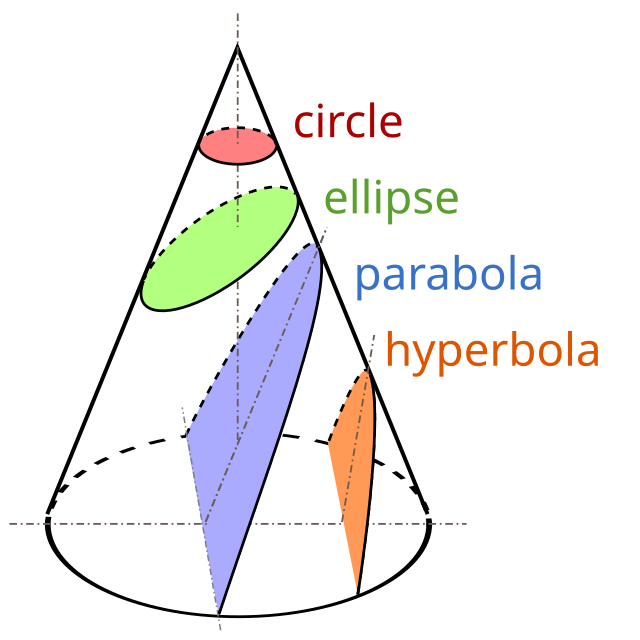
\includegraphics[width=0.4\textwidth]{chapters/chp1_pics/Conic_Sections.svg.png}
\caption{\textit{Conic sections derived from a single-napped cone. The hyperbola includes an additional section, as the intersecting plane extends through the origin to cut both nappes of the cone when there are two present.}}

    \label{fig:conic_sections}
\end{figure}



These curves can all be described by the general quadratic equation in two dimensions:
\[
Ax^2 + Bxy + Cy^2 + Dx + Ey + F = 0,
\]
where \( A, B, C, D, E, F \) are constants. By varying these constants, we generate the different conic sections. \\ \\ A natural question arises: \textit{How can we extend the idea of conic sections to three dimensions?} If conic sections are formed by the intersection of a plane with a cone, what would happen if we instead consider the intersection of a plane with a "generalized" three-dimensional quadratic surface? What kinds of shapes might we discover in three dimensions? These questions lead us to quadric surfaces. \\ \\ In three dimensions, the general equation for a quadric surface is:
\[
Ax^2 + By^2 + Cz^2 + Dxy + Exz + Fyz + Gx + Hy + Iz + J = 0,
\]
where \( A, B, C, D, E, F, G, H, I, J \) are constants. By adjusting these constants, we can produce a variety of surfaces, such as ellipsoids, hyperboloids, and paraboloids. Each surface is a natural extension of the conic sections, generalized to three-dimensional space. One of the most fascinating aspects of quadric surfaces is the diversity of shapes they produce. Why do we get surfaces as different as spheres, hyperboloids, and paraboloids from a single quadratic equation? Are these shapes related to one another? The answer lies in the interplay between the coefficients in the general equation and the symmetry of the surface.

\noindent To understand this, let us focus on the terms in the quadratic equation:
\[
Ax^2 + By^2 + Cz^2 + Dxy + Exz + Fyz + Gx + Hy + Iz + J = 0.
\]

\begin{itemize}
    \item \textbf{Symmetry and Dominance of Quadratic Terms:} The coefficients \( A, B, \) and \( C \) determine the relative ``stretching" or ``shrinking" along the \( x \)-, \( y \)-, and \( z \)-axes. For example, if \( A, B, \) and \( C \) are all positive, the surface is ``elliptical" in nature, producing shapes like spheres or ellipsoids. If one of these coefficients is negative, the surface takes on a "hyperbolic" character.
    
    \item \textbf{Mixed Terms:} The presence of mixed terms like \( Dxy, Exz, \) or \( Fyz \) introduces asymmetry into the surface. These terms ``tilt" the surface or create interactions between axes that result in more complex geometries.

    \item \textbf{Linear Terms:} The linear terms \( Gx, Hy, Iz \) shift the surface in space, altering its position without changing its overall shape.

    \item \textbf{Constant Term:} The constant \( J \) determines whether the surface passes through the origin or is offset.
\end{itemize}

\noindent The diversity of shapes arises from how these terms combine. For example:
\begin{itemize}
    \item A sphere occurs when \( A = B = C \), and all other terms vanish.
    \item An ellipsoid occurs when \( A, B, C > 0 \), but \( A \neq B \neq C \), and all mixed terms vanish.
    \item A hyperboloid arises when one of \( A, B, \) or \( C \) is negative, creating the distinctive ``saddle" or ``double-sheeted" structure.
\end{itemize}

\noindent Mathematically, these surfaces are related because they share the same fundamental structure: all are solutions to quadratic equations in three variables. By varying the coefficients and constants in the equation, we transition smoothly from one surface type to another.


\noindent To visualize why these shapes differ, think of a quadric surface as a collection of cross-sections. For example:
\begin{itemize}
    \item Setting \( z = k \) in the equation of a quadric surface gives a two-dimensional curve (a conic section) in the \( xy \)-plane. As \( k \) varies, these curves ``stack up" to form the three-dimensional surface.
    \item Similarly, setting \( x = k \) or \( y = k \) provides cross-sections in the \( yz \)- and \( xz \)-planes.
\end{itemize}

\noindent By examining these cross-sections, we can see how the different shapes arise:
\begin{itemize}
    \item For an ellipsoid, every cross-section is an ellipse, regardless of the plane.
    \item For a hyperboloid, some cross-sections are hyperbolas, while others are ellipses.
    \item For a paraboloid, cross-sections are parabolas in one direction and ellipses in another.
\end{itemize}

\noindent This perspective highlights the deep connection between conic sections and quadric surfaces: quadric surfaces are essentially ``stacks" of conic sections in three dimensions.

\subsubsection*{Preview of Multivariate Functions}

\noindent While our primary focus here is on the geometric nature of quadric surfaces, these surfaces also serve as important examples of multivariate functions. For instance, the equation of an elliptic paraboloid:
\[
\frac{x^2}{a^2} + \frac{y^2}{b^2} = z
\]
can be interpreted as the graph of the function \( z = f(x, y) \). Similarly, hyperbolic paraboloids and other quadric surfaces appear as graphs of functions with more complex structures.

\noindent Understanding quadric surfaces geometrically will prepare us to study multivariate functions rigorously in future lectures, where we will explore topics like partial derivatives, gradients, and optimization.


\subsection*{The Significance of Quadric Surfaces}

\noindent Quadric surfaces derive their name from the quadratic equations that define them. However, you might wonder: \textit{Why do we add the suffix ``-oid" to names like ellipsoid, paraboloid, and hyperboloid?} The term ``-oid" comes from the Greek word \textit{oides}, meaning ``like" or ``resembling." This suffix reflects the idea that quadric surfaces are three-dimensional analogs of their two-dimensional counterparts, the conic sections. 

\noindent For example:
\begin{itemize}
    \item An \textbf{ellipsoid} is ``like" an ellipse but extends into three dimensions.
    \item A \textbf{paraboloid} is ``like" a parabola but curves in three-dimensional space.
    \item A \textbf{hyperboloid} is ``like" a hyperbola, forming a saddle-shaped or double-sheeted surface in three dimensions.
\end{itemize}

\noindent This connection emphasizes the role of quadric surfaces as natural extensions of conic sections. While conic sections arise as intersections of a plane with a cone in two dimensions, quadric surfaces can be thought of as ``generalized" cones or cylinders in three dimensions.

\noindent \textbf{Why Are Quadric Surfaces Important?} These surfaces form the foundation for multivariate functions because they provide simple models for more complex phenomena. The symmetry inherent in quadric surfaces makes them ideal for representing many physical systems and mathematical problems. Consider the following examples:
\begin{itemize}
    \item \textbf{Paraboloids:} The surface of a satellite dish is a paraboloid, which focuses signals to a single point. Similarly, the shape of a suspension bridge cable under uniform load approximates a paraboloid.
    \item \textbf{Ellipsoids:} The orbits of some planets and the shape of Earth (approximated as an oblate spheroid) can be modeled using ellipsoids.
    \item \textbf{Hyperboloids:} Certain cooling towers, telescopes, and lenses rely on hyperboloids for their structural and optical properties.
\end{itemize}

\noindent Beyond these applications, quadric surfaces are central to \textbf{optimization problems}. They often appear as the contours of multivariate functions, where the geometry of the surface reveals key insights into the behavior of the function. For instance, an elliptic paraboloid can represent a local minimum, while a hyperbolic paraboloid can represent a saddle point.


\subsection*{Equations of Quadric Surfaces}

\noindent Let us first consider the simplest cases of quadric surfaces and slowly generalize to more complex ones. We will examine each surface type systematically, deriving its equation and visualizing its geometry.

\subsubsection*{Ellipsoids}

\noindent An ellipsoid is a natural three-dimensional extension of an ellipse. It is a surface defined by the equation:
\[
\frac{x^2}{a^2} + \frac{y^2}{b^2} + \frac{z^2}{c^2} = 1,
\]
where \( a, b, c > 0 \) are constants that determine the lengths of the semi-axes along the \( x \)-, \( y \)-, and \( z \)-axes, respectively. To understand this equation intuitively, let us set \( z = 0 \). The equation reduces to:
\[
\frac{x^2}{a^2} + \frac{y^2}{b^2} = 1,
\]
which represents an ellipse in the \( xy \)-plane. Similarly, setting \( y = 0 \) gives:
\[
\frac{x^2}{a^2} + \frac{z^2}{c^2} = 1,
\]
an ellipse in the \( xz \)-plane. Thus, the ellipsoid can be thought of as a ``stack" of ellipses in different planes.

\subsubsection*{Hyperboloids}

\noindent A hyperboloid comes in two varieties: one-sheeted and two-sheeted.

\paragraph{One-Sheeted Hyperboloid:} The equation for a one-sheeted hyperboloid is:
\[
\frac{x^2}{a^2} + \frac{y^2}{b^2} - \frac{z^2}{c^2} = 1.
\]
\noindent Here, the negative term (\( -\frac{z^2}{c^2} \)) causes the surface to open outward, creating a ``saddle-like" shape. Setting \( z = 0 \) reduces the equation to:
\[
\frac{x^2}{a^2} + \frac{y^2}{b^2} = 1,
\]
an ellipse in the \( xy \)-plane. However, as \( z \) increases or decreases, the cross-sections remain ellipses but grow larger, giving the hyperboloid its distinctive shape.

\paragraph{Two-Sheeted Hyperboloid:} The equation for a two-sheeted hyperboloid is:
\[
\frac{x^2}{a^2} + \frac{y^2}{b^2} - \frac{z^2}{c^2} = -1.
\]
\noindent This equation is similar to that of the one-sheeted hyperboloid, but here the minus sign on the right-hand side creates two disconnected surfaces, or ``sheets," opening in opposite directions. Setting \( z = 0 \) results in no real solutions, which explains the gap between the two sheets.






\subsubsection*{Elliptic Paraboloid}

\noindent The elliptic paraboloid is defined by the equation:
\[
\frac{x^2}{a^2} + \frac{y^2}{b^2} = z.
\]
\noindent To understand why we call this surface an \textit{elliptic paraboloid}, let us analyze its cross-sections:
\begin{itemize}
    \item Setting \( z = k \), where \( k > 0 \), reduces the equation to:
    \[
    \frac{x^2}{a^2} + \frac{y^2}{b^2} = k,
    \]
    which is the equation of an ellipse in the \( xy \)-plane. As \( z \) increases, these ellipses grow larger, creating a ``bowl-like" shape that opens upwards.
    \item On the other hand, setting \( x = k_1 \) or \( y = k_2 \) (for fixed constants \( k_1, k_2 \)) gives parabolas in the \( yz \)- or \( xz \)-plane, respectively. These parabolas describe how the surface curves along the vertical direction.
\end{itemize}
\noindent The name \textit{elliptic paraboloid} reflects the dual nature of this surface:
\begin{itemize}
    \item The term ``elliptic" comes from the elliptical cross-sections in the \( xy \)-plane.
    \item The term ``paraboloid" signifies that the surface extends like a parabola in the vertical direction.
\end{itemize}
\noindent This combination of elliptical and parabolic characteristics is the hallmark of an elliptic paraboloid.

\subsubsection*{Hyperbolic Paraboloid}

\noindent The hyperbolic paraboloid, often called a ``saddle surface," is defined by the equation:
\[
\frac{x^2}{a^2} - \frac{y^2}{b^2} = z.
\]
\noindent To understand the naming of this surface, let us examine its structure:
\begin{itemize}
    \item Setting \( z = k \) (for any constant \( k \)) reduces the equation to:
    \[
    \frac{x^2}{a^2} - \frac{y^2}{b^2} = k,
    \]
    which represents hyperbolas in the \( xy \)-plane when \( k \neq 0 \). These hyperbolas change orientation depending on the sign of \( k \): 
    \begin{itemize}
        \item For \( k > 0 \), the hyperbolas open along the \( x \)-axis.
        \item For \( k < 0 \), the hyperbolas open along the \( y \)-axis.
    \end{itemize}
    \item When \( z = 0 \), the equation becomes:
    \[
    \frac{x^2}{a^2} - \frac{y^2}{b^2} = 0,
    \]
    which simplifies to two intersecting lines, \( y = \pm \frac{b}{a}x \), in the \( xy \)-plane.
    \item Setting \( x = k_1 \) or \( y = k_2 \) (for fixed constants \( k_1, k_2 \)) gives parabolas in the \( yz \)- or \( xz \)-plane, respectively. These parabolas curve in opposite directions, creating the characteristic "saddle" shape.
\end{itemize}

\noindent The name \textit{hyperbolic paraboloid} reflects the surface's dual nature:
\begin{itemize}
    \item The term ``hyperbolic" comes from the hyperbolic cross-sections in the \( xy \)-plane.
    \item The term ``paraboloid" signifies that the surface contains parabolic cross-sections along the \( xz \)- and \( yz \)-planes.
\end{itemize}

\noindent The hyperbolic paraboloid's unique combination of upward and downward curvature makes it a saddle surface, giving it a distinct role in geometry and multivariable calculus.


\subsubsection*{Cylinders}

\noindent Cylinders are unique among quadric surfaces because they extend infinitely in one direction while maintaining a consistent cross-sectional shape in the other two dimensions. A cylinder can be thought of as the ``extrusion" of a conic section along an axis. The simplest form of a cylinder is the circular cylinder, given by:
\[
x^2 + y^2 = r^2,
\]
where \( r \) is the radius. While this equation might appear two-dimensional, it is not. The apparent ``two-dimensional" nature arises because the equation describes the cross-sectional shape of the cylinder in the \( xy \)-plane when \( z = 0 \). The cylinder itself is three-dimensional, extending infinitely in the \( z \)-direction. Setting \( z = k \) for any \( k \) gives circular cross-sections of radius \( r \) in the \( xy \)-plane at that height. More generally, a cylinder can take on other cross-sectional shapes, such as ellipses or parabolas. For example:
\begin{itemize}
    \item An \textbf{elliptic cylinder} is defined by:
    \[
    \frac{x^2}{a^2} + \frac{y^2}{b^2} = 1,
    \]
    which forms an ellipse in the \( xy \)-plane and extends infinitely in the \( z \)-direction.
    \item A \textbf{parabolic cylinder} is defined by:
    \[
    y = ax^2,
    \]
    which forms a parabola in the \( xy \)-plane and extends infinitely in the \( z \)-direction.
\end{itemize}

\noindent Cylinders are significant because they introduce the idea of surfaces that are not entirely bounded but still exhibit a clear geometric structure. They also help bridge the gap between two-dimensional conic sections and three-dimensional quadric surfaces.


\subsubsection*{Cones}

\noindent A cone is defined by the equation:
\[
\frac{x^2}{a^2} + \frac{y^2}{b^2} = \frac{z^2}{c^2}.
\]
\noindent Setting \( z = k \), where \( k \neq 0 \), reduces the equation to:
\[
\frac{x^2}{a^2} + \frac{y^2}{b^2} = k^2,
\]
an ellipse in the \( xy \)-plane. At \( z = 0 \), the equation reduces to a single point (the vertex of the cone). 


\subsubsection*{Visualization}
The below visual are what these quadric surfaces look like:



\begin{figure}[H]
    \centering
    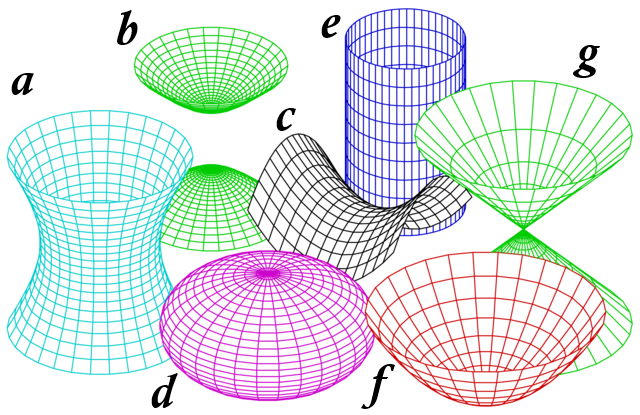
\includegraphics[width=0.8\textwidth]{chapters/chp1_pics/quadric_label.png}
    \caption{\textit{Assorted quadric surfaces.}}
    \label{fig:quadric_surfaces}
\end{figure}

\noindent The labeled surfaces are as follows:
\begin{enumerate}
    \item[a.] \textbf{Hyperboloid of One Sheet:} \( \frac{x^2}{a^2} + \frac{y^2}{b^2} - \frac{z^2}{c^2} = 1 \)
    \item[b.] \textbf{Hyperboloid of Two Sheets:} \( -\frac{x^2}{a^2} - \frac{y^2}{b^2} + \frac{z^2}{c^2} = 1 \)
    \item[c.] \textbf{Hyperbolic Paraboloid:} \( \frac{x^2}{a^2} - \frac{y^2}{b^2} = z \)
    \item[d.] \textbf{Ellipsoid:} \( \frac{x^2}{a^2} + \frac{y^2}{b^2} + \frac{z^2}{c^2} = 1 \)
    \item[e.] \textbf{Cylinder:} \( x^2 + y^2 = r^2 \)
    \item[f.] \textbf{Elliptic Paraboloid:} \( \frac{x^2}{a^2} + \frac{y^2}{b^2} = z \)
    \item[g.] \textbf{Elliptic Cone:} \( \frac{x^2}{a^2} + \frac{y^2}{b^2} - \frac{z^2}{c^2} = 0 \)
\end{enumerate}



\noindent To further explore the concepts of quadric surfaces, let us introduce a Python program that allows you to visualize these surfaces by manipulating their coefficients. By adjusting the parameters \( A, B, C, \) etc., you can observe how the shape and orientation of the surface changes. This hands-on approach helps build intuition about these mathematical objects.


\vspace{1.3em}


\begin{lstlisting}[language=Python]
import numpy as np
import matplotlib.pyplot as plt
from mpl_toolkits.mplot3d import Axes3D

# Define the function for the quadric surface
def quadric_surface(x, y, A, B, C, D, E, F, G, H, I, J):
    return A*x**2 + B*y**2 + C*(x*y) + D*x + E*y + F  # Replace or expand as needed

# Coefficients (students can modify these to observe changes)
A, B, C = 1, 1, 0
D, E, F = 0, 0, -1

# Create a meshgrid for the surface
x = np.linspace(-2, 2, 100)
y = np.linspace(-2, 2, 100)
x, y = np.meshgrid(x, y)

# Compute z-values for the surface
z = quadric_surface(x, y, A, B, C, D, E, F, 0, 0, 0, 0)

# Plot the surface
fig = plt.figure(figsize=(8, 6))
ax = fig.add_subplot(111, projection='3d')
ax.plot_surface(x, y, z, cmap="viridis", alpha=0.8)

# Labels and title
ax.set_xlabel('X-axis')
ax.set_ylabel('Y-axis')
ax.set_zlabel('Z-axis')
ax.set_title('Quadric Surface Visualization')

plt.show()
\end{lstlisting}

\vspace{1.3em}

\noindent \textbf{How to Use:} 
\begin{enumerate}
    \item Copy and paste the code into a Python environment, such as Jupyter Notebook or an IDE.
    \item Experiment with different values of the coefficients \( A, B, C, D, E, F, \) etc., to explore different quadric surfaces (e.g., ellipsoids, hyperboloids, paraboloids).
    \item Observe how the surface changes in response to these adjustments and compare it with the equations we’ve discussed in this lecture.
\end{enumerate}

\noindent This interactive approach not only reinforces your understanding of quadric surfaces but also demonstrates how algebraic changes in the equation correspond to geometric changes in the graph.


\exampleline
\begin{example}
\textbf{Visualizing the Intersection of a Plane and a Quadric Surface}

\noindent Consider the quadric surface given by:
\[
\frac{x^2}{4} + \frac{y^2}{9} - \frac{z^2}{16} = 1,
\]
which is a hyperboloid of one sheet. Let the intersecting plane be defined by \( z = 2 \). Find the resulting curve of intersection.

\begin{solution}

\noindent To find the intersection, substitute \( z = 2 \) into the equation of the hyperboloid:
\[
\frac{x^2}{4} + \frac{y^2}{9} - \frac{(2)^2}{16} = 1.
\]

\noindent Simplify the \( z^2 \) term:
\[
\frac{x^2}{4} + \frac{y^2}{9} - \frac{4}{16} = 1 \quad \implies \quad \frac{x^2}{4} + \frac{y^2}{9} - \frac{1}{4} = 1.
\]

\noindent Rearrange:
\[
\frac{x^2}{4} + \frac{y^2}{9} = \frac{5}{4}.
\]

\noindent Multiply through by 36 (the least common multiple of 4 and 9) to clear the denominators:
\[
9x^2 + 4y^2 = 45.
\]

\noindent This is the equation of an ellipse in the \( xy \)-plane. The plane \( z = 2 \) intersects the hyperboloid to form an ellipse at this height.

\noindent \textbf{Summary:} The curve of intersection between the hyperboloid \( \frac{x^2}{4} + \frac{y^2}{9} - \frac{z^2}{16} = 1 \) and the plane \( z = 2 \) is:
\[
9x^2 + 4y^2 = 45.
\]
This describes an ellipse in the \( xy \)-plane when viewed at \( z = 2 \).

\end{solution}
\end{example}




\exampleline

\begin{example}
\textbf{Classifying a Quadric Surface by Its Equation}

\noindent Given the equation:
\[
\frac{x^2}{9} + \frac{y^2}{4} + \frac{z^2}{16} = 1,
\]
identify the type of quadric surface and describe its geometric properties.

\begin{solution}

\noindent The given equation is of the form:
\[
\frac{x^2}{a^2} + \frac{y^2}{b^2} + \frac{z^2}{c^2} = 1,
\]
where \( a^2 = 9 \), \( b^2 = 4 \), and \( c^2 = 16 \). Since all the terms are positive and equal to 1 on the right-hand side, this is an \textbf{ellipsoid}.

\noindent \textbf{Geometric Properties:}
\begin{itemize}
    \item The center of the ellipsoid is at \( (0, 0, 0) \), as there are no linear terms in \( x, y, \) or \( z \).
    \item The semi-axes of the ellipsoid are aligned with the coordinate axes:
    \[
    a = 3, \quad b = 2, \quad c = 4.
    \]
    \item The semi-axis lengths \( a, b, c \) define the radii of the ellipsoid along the \( x, y, \) and \( z \)-axes, respectively.
\end{itemize}

\noindent \textbf{Summary:} The equation \( \frac{x^2}{9} + \frac{y^2}{4} + \frac{z^2}{16} = 1 \) represents an ellipsoid centered at the origin with semi-axes of lengths 3, 2, and 4 along the \( x, y, \) and \( z \)-axes.

\end{solution}
\end{example}






\exampleline

\begin{example}
\textbf{Finding the Intersection Between a Cylinder and a Plane}

\noindent Consider the cylinder:
\[
x^2 + y^2 = 9,
\]
and the plane \( z = 3x + y \). Find the parametric equations for their intersection.

\begin{solution}

\noindent This example introduces a new technique for working with nonlinear equations. Previously, we dealt with linear parameterizations for lines and planes. Here, we parameterize a \textit{circle} in the \( xy \)-plane, which is inherently nonlinear.  \\ \\ The cylinder is defined by \( x^2 + y^2 = 9 \). This equation represents a circle in the \( xy \)-plane with radius 3. To parameterize the circle, we note that for a unit circle, the coordinates of points on the circle can be written as \( x = \cos t \) and \( y = \sin t \), where \( t \) is the angle swept counterclockwise from the positive \( x \)-axis. Scaling this relationship to a circle of radius \( r \) gives:
\[
x = r \cos t, \quad y = r \sin t,
\]
where \( t \in [0, 2\pi) \) describes the angle around the circle. Substituting \( r = 3 \), we have:
\[
x = 3 \cos t, \quad y = 3 \sin t, \quad t \in [0, 2\pi).
\]
This parameterization allows us to represent all points on the circle in the \( xy \)-plane as \( t \) varies from \( 0 \) to \( 2\pi \).

\noindent The plane \( z = 3x + y \) provides the \( z \)-coordinate for each point of the intersection. Substituting the parameterized values of \( x \) and \( y \) into the plane equation:
\[
z = 3x + y \implies z = 3(3 \cos t) + 3 \sin t = 9 \cos t + 3 \sin t.
\]

\noindent Thus, the parametric equations for the curve of intersection are:
\[
x = 3 \cos t, \quad y = 3 \sin t, \quad z = 9 \cos t + 3 \sin t, \quad t \in [0, 2\pi).
\]

\noindent \textbf{Key Insight:} Nonlinear equations like \( x^2 + y^2 = 9 \) can often be parameterized using trigonometric functions (\( \cos t \) and \( \sin t \)), leveraging their geometric relationship with circles. While the equations may appear two-dimensional initially, the \( z \)-coordinate from the plane adds a third dimension to the curve of intersection, creating a space curve. \\ \\ \textbf{Summary:} The curve of intersection between the cylinder \( x^2 + y^2 = 9 \) and the plane \( z = 3x + y \) is a space curve parameterized by:
\[
x = 3 \cos t, \quad y = 3 \sin t, \quad z = 9 \cos t + 3 \sin t, \quad t \in [0, 2\pi).
\]

\end{solution}
\end{example}
\exampleline


\newpage


\formsdefs{}

\subsection*{Important Vocabulary}
\begin{itemize}
    \item \textbf{Cartesian Coordinates:} A system to define points in three-dimensional space using \((x, y, z)\).
    \item \textbf{Cylindrical Coordinates:} Defined by \((r, \theta, z)\), where \(r\) is the radial distance, \(\theta\) the angle from the positive \(x\)-axis, and \(z\) the height.
    \item \textbf{Spherical Coordinates:} Represented as \((\rho, \theta, \phi)\), where \(\rho\) is the radial distance, \(\theta\) the azimuthal angle, and \(\phi\) the polar angle.
    \item \textbf{Vector:} A quantity with both magnitude and direction, expressed as \(\mathbf{v} = \langle v_x, v_y, v_z \rangle\).
    \item \textbf{Dot Product:} A scalar product of two vectors, given by \(\mathbf{u} \cdot \mathbf{v} = u_x v_x + u_y v_y + u_z v_z\).
    \item \textbf{Cross Product:} A vector perpendicular to two vectors, calculated using the determinant of a \(3 \times 3\) matrix.
    \item \textbf{Parallelepiped:} A six-faced figure formed by three vectors, where its volume is given by the scalar triple product \(|\mathbf{u} \cdot (\mathbf{v} \times \mathbf{w})|\).
\end{itemize}

\subsection*{Key Formulas}
\begin{multicols}{2}
\paragraph{Distance Formula in 3D:}
\[
d = \sqrt{(x_2 - x_1)^2 + (y_2 - y_1)^2 + (z_2 - z_1)^2}
\]

\paragraph{Midpoint Formula:}
\[
M = \left(\frac{x_1 + x_2}{2}, \frac{y_1 + y_2}{2}, \frac{z_1 + z_2}{2}\right)
\]

\paragraph{Direction Cosines:} \index{Direction Cosines}
\[
\begin{aligned}
\cos \alpha &= \frac{u_x}{|\mathbf{u}|}, \quad
\cos \beta = \frac{u_y}{|\mathbf{u}|}, \\
\cos \gamma &= \frac{u_z}{|\mathbf{u}|}
\end{aligned}
\]
where $\cos^2 \alpha + \cos^2 \beta + \cos^2 \gamma = 1$

\paragraph{Angle Between Vectors:} \index{Vector Angle}
\[
\cos \theta = \frac{\mathbf{u} \cdot \mathbf{v}}{|\mathbf{u}||\mathbf{v}|}, \quad
\sin \theta = \frac{|\mathbf{u} \times \mathbf{v}|}{|\mathbf{u}||\mathbf{v}|}
\]

\paragraph{Dot Product:}
\[
\mathbf{u} \cdot \mathbf{v} = u_x v_x + u_y v_y + u_z v_z
\]

\paragraph{Cross Product:}
\begin{align*}
\mathbf{u} \times \mathbf{v} &= \begin{vmatrix}
\mathbf{i} & \mathbf{j} & \mathbf{k} \\
u_x & u_y & u_z \\
v_x & v_y & v_z
\end{vmatrix} \\
&= \mathbf{i}(u_y v_z - u_z v_y) \\
&\quad - \mathbf{j}(u_x v_z - u_z v_x) \\
&\quad + \mathbf{k}(u_x v_y - u_y v_x)
\end{align*}

\paragraph{Parametric Line:} \index{Parametric Line}
\[
\mathbf{r}(t) = \mathbf{P}_0t + \mathbf{P}_1(1-t), \quad t \in [0,1]
\]
or alternatively:
\[
\mathbf{r}(t) = \mathbf{P}_0 + t\mathbf{v}, \quad t \in \mathbb{R}
\]

\paragraph{Volume of a Parallelepiped (Scalar Triple Product):}
\[
\text{Volume} = |\mathbf{u} \cdot (\mathbf{v} \times \mathbf{w})|
\]

\paragraph{Conversion Between Coordinates:}
\begin{itemize}
\item Cartesian to Cylindrical:
\[
\begin{aligned}
r &= \sqrt{x^2 + y^2}, \quad
\theta = \tan^{-1}\left(\frac{y}{x}\right), \\
z &= z
\end{aligned}
\]
\item Cartesian to Spherical:
\[
\begin{aligned}
\rho &= \sqrt{x^2 + y^2 + z^2}, \quad
\theta = \tan^{-1}\left(\frac{y}{x}\right), \\
\phi &= \cos^{-1}\left(\frac{z}{\rho}\right)
\end{aligned}
\]
\item Cylindrical to Cartesian:
\[
\begin{aligned}
x &= r \cos \theta, \quad
y = r \sin \theta, \\
z &= z
\end{aligned}
\]
\item Spherical to Cartesian:
\[
\begin{aligned}
x &= \rho \sin \phi \cos \theta, \quad
y = \rho \sin \phi \sin \theta, \\
z &= \rho \cos \phi
\end{aligned}
\]
\end{itemize}

\paragraph{Plane Equation:}
\[
Ax + By + Cz + D = 0
\]

\paragraph{Line Equation (Parametric Form):}
\[
\mathbf{r}(t) = \mathbf{v} + t \mathbf{d}
\]

\paragraph{Quadratic Surfaces:}
\begin{itemize}
    \item \textbf{Ellipsoid:} \(\frac{x^2}{a^2} + \frac{y^2}{b^2} + \frac{z^2}{c^2} = 1\)
    \item \textbf{Hyperboloid of One Sheet:} \(\frac{x^2}{a^2} + \frac{y^2}{b^2} - \frac{z^2}{c^2} = 1\)
    \item \textbf{Hyperboloid of Two Sheets:} \(-\frac{x^2}{a^2} - \frac{y^2}{b^2} + \frac{z^2}{c^2} = 1\)
    \item \textbf{Elliptic Paraboloid:} \(\frac{x^2}{a^2} + \frac{y^2}{b^2} = z\)
\end{itemize}
\end{multicols}



\newpage

\practice{}

\begin{multicols}{2}

\begin{enumerate}
    % Calculus 1 and 2 Review (10 Questions)
    \item Differentiate the function \( f(t) = t^3 + \sin(t) + e^t \) with respect to \( t \).
    \item Compute the limit \( \lim_{t \to 0} \frac{\sin(t)}{t} \).
    \item Integrate the function \( f(t) = 2t + 3 \) with respect to \( t \).
    \item Find the critical points of \( f(t) = t^4 - 4t^3 + 6t^2 - 4t + 1 \).
    \item Determine the interval of convergence for the power series \( \sum_{n=0}^{\infty} \frac{x^n}{n!} \).
    \item Evaluate the improper integral \( \int_{1}^{\infty} \frac{1}{x^2} \, dx \).
    \item Find the Taylor series of \( e^x \) centered at \( x = 0 \) up to the \( x^3 \) term.
    \item Compute \( \lim_{x \to \infty} \frac{2x^3 - x + 1}{x^3 + 4x^2} \).
    \item Solve the optimization problem: Find the maximum area of a rectangle inscribed under the curve \( y = 4 - x^2 \).
    \item A ladder 10 feet long is leaning against a wall. If the base of the ladder is pulled away from the wall at a rate of 2 feet per second, how fast is the top of the ladder descending when the base is 6 feet from the wall?

    % Three-Dimensional Coordinate Systems (14 Questions)
    \item Convert the rectangular coordinates \( (x, y, z) = (3, -3, 3) \) to spherical coordinates.
    \item Find the rectangular coordinates of the point with cylindrical coordinates \( (r, \theta, z) = \left(2, \dfrac{\pi}{4}, -1\right) \).
    \item Determine the distance between the points \( (2, -1, 4) \) and \( (-3, 5, -2) \) in three-dimensional space.
    \item Express the spherical coordinates \( (\rho, \theta, \phi) = \left(5, \dfrac{\pi}{3}, \dfrac{\pi}{6}\right) \) in rectangular coordinates.
    \item Convert the point \( (x, y, z) = (-4, 4, \sqrt{3}) \) from rectangular to cylindrical coordinates.
    \item Find the midpoint between the points \( (1, 2, 3) \) and \( (-1, -2, -3) \) in three-dimensional space.
    \item Determine the angle between the positive \( x \)-axis and the projection of the vector \( \mathbf{v} = \langle 3, 3, 3 \rangle \) onto the \( xy \)-plane.
    \item Convert the rectangular coordinates \( (0, -5, 5) \) to spherical coordinates.
    \item Find the cylindrical coordinates of the point \( (x, y, z) = (2\sqrt{2}, 2\sqrt{2}, -3) \).
    \item Determine the spherical coordinates of the point \( (x, y, z) = (-2, -2, 2\sqrt{2}) \).
    \item Express the point \( (\rho, \theta, \phi) = \left(6, \dfrac{2\pi}{3}, \dfrac{\pi}{4}\right) \) in rectangular coordinates.
    \item Convert the cylindrical coordinates \( (r, \theta, z) = \left(3, \dfrac{\pi}{6}, 4\right) \) to spherical coordinates.
    \item Find the rectangular coordinates of the point \( (r, \theta, z) = \left(1, \dfrac{\pi}{2}, -2\right) \).
    \item Determine the distance from the origin to the point \( (x, y, z) = (a, b, c) \) in rectangular coordinates.
    \item Convert the point \( (x, y, z) = (0, 0, 0) \) to spherical coordinates.

    % Vectors (19 Questions)
    \item Compute \( |\mathbf{v}| \) for \( \mathbf{v} = \langle 3, -4, 5 \rangle \).
    \item Find the unit vector in the direction of \( \mathbf{v} = \langle -2, 1, 3 \rangle \).
    \item Calculate \( \mathbf{u} \cdot \mathbf{v} \) for \( \mathbf{u} = \langle 1, 2, 3 \rangle \) and \( \mathbf{v} = \langle 4, 0, -1 \rangle \).
    \item Determine \( \mathbf{u} \times \mathbf{v} \) for \( \mathbf{u} = \langle 1, 0, -1 \rangle \) and \( \mathbf{v} = \langle 0, 2, 3 \rangle \).
    \item Find the angle between \( \mathbf{u} = \langle 1, 2, 3 \rangle \) and \( \mathbf{v} = \langle 3, 2, 1 \rangle \).
    \item Show that \( \mathbf{u} = \langle 2, -1, 0 \rangle \) and \( \mathbf{v} = \langle 4, -2, 0 \rangle \) are \textit{linearly dependent} (meaning that one cannot be written as a constant multiple of the other).
    \item Compute the area of the parallelogram spanned by \( \mathbf{u} = \langle 1, 0, 1 \rangle \) and \( \mathbf{v} = \langle 0, 2, 1 \rangle \).
    \item Find a vector orthogonal to both \( \mathbf{u} = \langle 1, -1, 0 \rangle \) and \( \mathbf{v} = \langle 2, 1, -1 \rangle \).
    \item Determine if the vectors \( \mathbf{a} = \langle 3, -1, 2 \rangle \), \( \mathbf{b} = \langle 4, 0, -2 \rangle \), and \( \mathbf{c} = \langle 1, 5, -1 \rangle \) are linearly independent.
    \item Find the projection of \( \mathbf{u} = \langle 4, -2, 1 \rangle \) onto \( \mathbf{v} = \langle 1, 0, 3 \rangle \).
    \item Calculate the scalar triple product \( \mathbf{a} \cdot (\mathbf{b} \times \mathbf{c}) \) for \( \mathbf{a} = \langle 1, 2, 3 \rangle \), \( \mathbf{b} = \langle 4, 5, 6 \rangle \), and \( \mathbf{c} = \langle 7, 8, 9 \rangle \).
    \item Find the volume of the parallelepiped formed by the vectors \( \mathbf{u} = \langle 1, 0, 0 \rangle \), \( \mathbf{v} = \langle 0, 1, 0 \rangle \), and \( \mathbf{w} = \langle 0, 0, 1 \rangle \).
    \item Determine the component of \( \mathbf{a} = \langle 5, 2, -3 \rangle \) along \( \mathbf{b} = \langle 1, -1, 2 \rangle \).
    \item Compute the magnitude of the vector \( \mathbf{w} = \mathbf{u} \times \mathbf{v} \) where \( \mathbf{u} = \langle 2, 3, 4 \rangle \) and \( \mathbf{v} = \langle -1, 0, 1 \rangle \).
    \item Find the angle between the vectors \( \mathbf{a} = \langle 2, -1, 3 \rangle \) and \( \mathbf{b} = \langle 1, 4, -2 \rangle \).
    \item Show that the vectors \( \mathbf{u} = \langle 1, 2, 3 \rangle \), \( \mathbf{v} = \langle 4, 5, 6 \rangle \), and \( \mathbf{w} = \langle 7, 8, 9 \rangle \) are \textit{coplanar} (are all on the same plane).
    \item Calculate the area of the triangle formed by the vectors \( \mathbf{u} = \langle 2, 0, -1 \rangle \) and \( \mathbf{v} = \langle 1, 3, 4 \rangle \).
    \item Find the vector projection of \( \mathbf{a} = \langle 3, -2, 1 \rangle \) onto \( \mathbf{b} = \langle 4, 0, -1 \rangle \).
    \item Determine if the vectors \( \mathbf{u} = \langle 2, 4, 6 \rangle \) and \( \mathbf{v} = \langle -1, -2, -3 \rangle \) are orthogonal.
    \item Compute the cross product \( \mathbf{u} \times \mathbf{v} \) for \( \mathbf{u} = \langle 0, 1, 2 \rangle \) and \( \mathbf{v} = \langle 3, 4, 5 \rangle \).
    \item Find the unit vector perpendicular to the plane defined by \( \mathbf{u} = \langle 1, 2, 3 \rangle \) and \( \mathbf{v} = \langle 4, 5, 6 \rangle \).
\item Determine whether the vectors \( \mathbf{a} = \langle 1, 2, 3 \rangle \), \( \mathbf{b} = \langle 2, 4, 6 \rangle \), and \( \mathbf{c} = \langle 3, 6, 9 \rangle \) are linearly independent or dependent. Linear independence means that none of the vectors can be written as a combination of the others, ie $v_1 \neq k_1 v_2 + k_2 v_3$. If at least one vector can be expressed as a combination of the others, the vectors are linearly dependent.
    \item Calculate the dot product \( \mathbf{u} \cdot \mathbf{v} \) for \( \mathbf{u} = \langle 5, -2, 4 \rangle \) and \( \mathbf{v} = \langle -1, 3, 2 \rangle \).
    \item Find the angle between the vectors \( \mathbf{u} = \langle 7, 0, -5 \rangle \) and \( \mathbf{v} = \langle 4, -3, 2 \rangle \).
    \item Show that the vectors \( \mathbf{u} = \langle 1, 3, -2 \rangle \) and \( \mathbf{v} = \langle 4, -1, 5 \rangle \) are not parallel.
    \item Compute the area of the parallelogram formed by \( \mathbf{u} = \langle 3, -1, 2 \rangle \) and \( \mathbf{v} = \langle -2, 4, 1 \rangle \).
    \item Find a vector orthogonal to \( \mathbf{u} = \langle 2, -3, 1 \rangle \) and \( \mathbf{v} = \langle 4, 0, -2 \rangle \).

    % Lines and Planes in Space (14 Questions)
    \item Find the equation of the line passing through \( (1, 0, -1) \) and \( (2, 3, 4) \).
    \item Determine the equation of the plane containing the points \( (1, 2, 3) \), \( (-1, 0, 4) \), and \( (3, -2, 1) \).
    \item Compute the point of intersection of the line \( \mathbf{r}(t) = \langle 1 + t, 2 - t, 3t \rangle \) with the plane \( x - y + z = 5 \).
    \item Check if the lines \( \mathbf{r}_1(t) = \langle t, 2t, 3t \rangle \) and \( \mathbf{r}_2(s) = \langle 1 + s, 2, 3s \rangle \) are parallel, intersecting, or skew.
    \item Given \( \Pi_1: x + 2y + 3z = 7 \), \( \Pi_2: -2x - y - z = 2 \), and \( \mathbf{r}(t) = \langle 2t, 1 - t, 1 + t \rangle \), determine if \( \mathbf{r}(t) \) intersects both planes. If so, calculate the length of \( \mathbf{r}(t) \) from \( \Pi_1 \) to \( \Pi_2 \).
    \item Find the shortest distance between the line \( \mathbf{r}(t) = \langle t, t, t \rangle \) and the point \( (1, 1, 1) \).
    \item Determine the equation of the line of intersection of the planes \( x + y + z = 1 \) and \( 2x - y + 3z = 4 \).
    \item Find the distance between the parallel planes \( x + 2y + 2z = 5 \) and \( x + 2y + 2z = -3 \).
    \item Find the parametric equations of the line perpendicular to the plane \( 3x - 2y + z = 7 \) and passing through the point \( (2, -1, 4) \).
    \item Determine the angle between the line \( \mathbf{r}(t) = \langle 1 + 2t, 3 - t, 4t \rangle \) and the plane \( 2x - 3y + z = 7 \).
    \item Find the equation of the plane perpendicular to the vector \( \mathbf{n} = \langle 3, -2, 5 \rangle \) and passing through the point \( (2, -1, 4) \).
    \item Compute the intersection curve of the sphere \( x^2 + y^2 + z^2 = 25 \) and the plane \( z = 3 \).
    \item Find the equation of a line that is parallel to the vector \( \mathbf{v} = \langle 2, -1, 3 \rangle \) and passes through the point \( (-1, 4, 2) \).
    \item Determine whether the lines \( \mathbf{r}_1(t) = \langle 1 + t, 2 - t, 3 + 2t \rangle \) and \( \mathbf{r}_2(s) = \langle 4 - s, -1 + s, 5 + s \rangle \) intersect.
    \item Compute the equation of the tangent plane to the surface \( x^2 + 2y^2 + 3z^2 = 6 \) at the point \( (1, 1, 1) \).
    \item Find the line segment of shortest length connecting the lines \( \mathbf{r}_1(t) = \langle t, 2t, 3t \rangle \) and \( \mathbf{r}_2(s) = \langle 1 + s, 2 + s, 3 + s \rangle \).
    \item Determine the parametric equations for the space curve defined by \( x = t \), \( y = \sin(t) \), and \( z = \cos(t) \).
    \item Find the intersection of the hyperboloid \( x^2 - y^2 - z^2 = 4 \) with the plane \( y = 1 \).
    \item Calculate the surface area of the cylinder \( x^2 + y^2 = 9 \) between \( z = 0 \) and \( z = 5 \).
    \item Find the equation of the ellipsoid with semi-axes of lengths 3, 4, and 5 along the \( x \)-, \( y \)-, and \( z \)-axes, respectively.
    \item Derive the Cartesian equation of the paraboloid obtained by rotating the parabola \( z = x^2 \) about the \( z \)-axis.
   \item As we have seen, the parametric equation of a line can be represented as $\mathbf{r}(t) = \mathbf{P}_0t + \mathbf{P}_1(1-t), \quad t \in [0,1]$. If we wanted to change $t$ to go between $0$ and $a \in \mathbb{R}^{+}$, how would our parametric equation change?

    % Quadric Surfaces (5 Questions)
    \item Classify the surface given by \( x^2 + y^2 - z^2 = 1 \).
    \item Write the parametric equations for the intersection of the cylinder \( x^2 + y^2 = 4 \) with the plane \( z = x + y \).
    \item Verify if the surface \( x^2 + y^2 - 4z = 0 \) is an elliptic paraboloid.
    \item Compute the volume enclosed by the sphere \( x^2 + y^2 + z^2 = 4 \) and the plane \( z = 1 \).
    \item Find the equation of the surface generated by rotating \( x = y^2 \) about the \( z \)-axis.

\end{enumerate}

\end{multicols}

